% Capitolul 1: Evaluarea prognozelor, reguli de scor și combinarea prognozelor
% Analiza avansată a seriilor de timp și previziune -- Programul de master Statistică aplicată și data science, anul I, semestrul 2, Academia de Studii Economice din București
% GENERAT de latex/build_chapter1.py -- modificați generatorul, nu acest fișier.

\newcommand{\coursename}{Analiza avansată a seriilor de timp și previziune}
\def\atslang{ro}
% Preambul comun ATS -- Analiza avansată a seriilor de timp și previziune / Advanced Time Series Analysis and Forecasting
% (Beamer, 16:9). Același design ca MFM, SFM și TSA (copiat din TSA, 5 octombrie 2026). Înainte de % Preambul comun ATS -- Analiza avansată a seriilor de timp și previziune / Advanced Time Series Analysis and Forecasting
% (Beamer, 16:9). Același design ca MFM, SFM și TSA (copiat din TSA, 5 octombrie 2026). Înainte de % Preambul comun ATS -- Analiza avansată a seriilor de timp și previziune / Advanced Time Series Analysis and Forecasting
% (Beamer, 16:9). Același design ca MFM, SFM și TSA (copiat din TSA, 5 octombrie 2026). Înainte de \input{../../latex/preamble} se definește
%   \newcommand{\coursename}{Advanced Time Series Analysis and Forecasting}          (EN)
%   \newcommand{\coursename}{Analiza avansată a seriilor de timp și previziune}       (RO)  și  \def\atslang{ro}
% Fișierele .tex se află în EN/Courses, EN/Seminars, RO/Cursuri, RO/Seminarii (două niveluri sub rădăcină).
% Deck-urile sînt generate de latex/build_chapterN.py / build_seminarN.py (vezi latex/ats_build.py).

\documentclass[9pt, aspectratio=169, t]{beamer}
\providecommand{\coursename}{Advanced Time Series Analysis and Forecasting}

% Ensure content fits on slides
\setbeamersize{text margin left=8mm, text margin right=8mm}
% Smaller institute font (title page)
\setbeamerfont{institute}{size=\footnotesize}

%=============================================================================
% THEME AND STYLE CONFIGURATION
%=============================================================================
\usetheme{default}
% Using default theme for clean header/footer control

% Color Palette (matching Redispatch PDF)
\definecolor{MainBlue}{RGB}{26, 58, 110}
\definecolor{AccentBlue}{RGB}{26, 58, 110}
\definecolor{IDAred}{RGB}{205, 0, 0}
\definecolor{DarkGray}{RGB}{51, 51, 51}
\definecolor{MediumGray}{RGB}{128, 128, 128}
\definecolor{LightGray}{RGB}{248, 248, 248}
\definecolor{VeryLightGray}{RGB}{235, 235, 235}
\definecolor{KeynoteGray}{RGB}{218, 218, 218}
\definecolor{SectionGray}{RGB}{120, 120, 120}
\definecolor{FooterGray}{RGB}{100, 100, 100}
\definecolor{Crimson}{RGB}{220, 53, 69}
\definecolor{Forest}{RGB}{46, 125, 50}
\definecolor{Amber}{RGB}{181, 133, 63}
\definecolor{Orange}{RGB}{230, 126, 34}
\definecolor{Purple}{RGB}{142, 68, 173}

% Gradient background (exact Keynote 315° gradient: white to RGB 218,218,218)
\setbeamertemplate{background}{%
    \begin{tikzpicture}[remember picture, overlay]
        \shade[shading=axis, shading angle=315,
        top color=white, bottom color=KeynoteGray]
        (current page.south west) rectangle (current page.north east);
    \end{tikzpicture}%
}
% Fallback solid color for compatibility
\setbeamercolor{background canvas}{bg=}

\setbeamercolor{palette primary}{bg=MainBlue, fg=white}
\setbeamercolor{palette secondary}{bg=MainBlue!85, fg=white}
\setbeamercolor{palette tertiary}{bg=MainBlue!70, fg=white}
\setbeamercolor{structure}{fg=MainBlue}
\setbeamercolor{title}{fg=IDAred}
\setbeamercolor{frametitle}{fg=IDAred, bg=}
\setbeamercolor{block title}{bg=MainBlue, fg=white}
\setbeamercolor{block body}{bg=VeryLightGray, fg=DarkGray}
\setbeamercolor{block title alerted}{bg=Crimson, fg=white}
\setbeamercolor{block body alerted}{bg=Crimson!8, fg=DarkGray}
\setbeamercolor{block title example}{bg=Forest, fg=white}
\setbeamercolor{block body example}{bg=Forest!8, fg=DarkGray}
\setbeamercolor{item}{fg=MainBlue}

% Footer colors (override Madrid theme blue)
\setbeamercolor{author in head/foot}{fg=FooterGray, bg=}
\setbeamercolor{title in head/foot}{fg=FooterGray, bg=}
\setbeamercolor{date in head/foot}{fg=FooterGray, bg=}
\setbeamercolor{section in head/foot}{fg=FooterGray, bg=}
\setbeamercolor{subsection in head/foot}{fg=FooterGray, bg=}

% Bullet styles (apply everywhere including blocks)
\setbeamertemplate{itemize item}{\color{MainBlue}$\boxdot$}
\setbeamertemplate{itemize subitem}{\color{MainBlue}$\blacktriangleright$}
\setbeamertemplate{itemize subsubitem}{\color{MainBlue}\tiny$\bullet$}
\setbeamertemplate{itemize/enumerate body begin}{\normalsize}
\setbeamertemplate{itemize/enumerate subbody begin}{\normalsize}

% Item spacing - compact style
\setlength{\leftmargini}{10pt}       % Level 1: minimal indent
\setlength{\leftmarginii}{10pt}      % Level 2: minimal additional indent
% Compact list spacing (zero extra space before/after lists in blocks)
\makeatletter
\def\@listi{\leftmargin\leftmargini \topsep 0pt \parsep 0pt \itemsep 0pt}
\def\@listii{\leftmargin\leftmarginii \topsep 0pt \parsep 0pt \itemsep 0pt}
\makeatother

\setbeamertemplate{navigation symbols}{}

%=============================================================================
% CUSTOM HEADLINE
%=============================================================================
\setbeamertemplate{headline}{%
    \vskip10pt%
    \hbox to \paperwidth{%
        \hskip0.5cm%
        {\small\color{FooterGray}\renewcommand{\hyperlink}[2]{##2}\insertsectionhead}%
        \hfill%
        \textcolor{FooterGray}{\small\insertframenumber}%
        \hskip0.5cm%
    }%
    \vskip4pt%
    {\color{FooterGray}\hrule height 0.4pt}%
}

%=============================================================================
% CUSTOM FOOTER
%=============================================================================
\usepackage{fontawesome5}

\setbeamertemplate{footline}{%
    {\color{FooterGray}\hrule height 0.4pt}%
    \vskip4pt%
    \hbox to \paperwidth{%
        \hskip0.5cm%
        \textcolor{FooterGray}{\small\coursename}%
        \hfill%
        \raisebox{-0.1em}{%
            \begin{tikzpicture}[x=0.08em, y=0.08em, line width=0.4pt]
                \draw[FooterGray] (0,3) -- (1,4) -- (2,3.5) -- (3,5) -- (4,4) -- (5,6) -- (6,5.5) -- (7,4) -- (8,5) -- (9,7) -- (10,6) -- (11,5) -- (12,6.5) -- (13,8) -- (14,7) -- (15,6) -- (16,7.5) -- (17,9) -- (18,8) -- (19,7) -- (20,8.5) -- (21,10) -- (22,9) -- (23,8) -- (24,9.5);
            \end{tikzpicture}%
        }%
        \hskip0.5cm%
    }%
    \vskip6pt%
}

%=============================================================================
% PACKAGES
%=============================================================================
\usepackage[utf8]{inputenc}
\DeclareUnicodeCharacter{03B1}{\ensuremath{\alpha}}
\usepackage[T1]{fontenc}
\usepackage{amsmath, amssymb, amsthm}
\usepackage{mathtools}
\usepackage{bm}
\usepackage{tikz}
\usetikzlibrary{arrows.meta, positioning, shapes, calc, decorations.pathreplacing, shadings}
\usepackage{booktabs}
\usepackage{multirow}
\usepackage{array}
\usepackage{graphicx}
\usepackage{animate}
\usepackage{hyperref}
\usepackage{colortbl}
\usepackage{listings}
\lstset{language=Python, basicstyle=\ttfamily\scriptsize, keywordstyle=\color{MainBlue}\bfseries,
  commentstyle=\color{Forest}, stringstyle=\color{Crimson}, breaklines=true,
  frame=none, backgroundcolor=\color{VeryLightGray}, xleftmargin=2mm}
\hypersetup{colorlinks=true, linkcolor=MainBlue, urlcolor=MainBlue}
\graphicspath{{../../logos/}{../../charts/}{../../photos/}}
\usepackage{xcolor}
\hfuzz=2pt  % Suppress tiny overfull warnings (<2pt)
\vfuzz=2pt  % Suppress tiny vertical overfull warnings (<2pt)

%=============================================================================
% QUANTLET COMMANDS
%   \quantlet{<displayed name>}{<url>}       (generic)
%   \atsquantlet{Ch_05}{ATS_ch5_garch}       -> https://github.com/danpele/Advanced-Time-Series/tree/main/Quantlets/Ch_05/ATS_ch5_garch
%   \qlurl{<folder>} is defined per chapter by the generator (Quantlets/Ch_NN/<folder>)
%=============================================================================
\newcommand{\atsrepo}{https://github.com/danpele/Advanced-Time-Series}
\newcommand{\atsqlbase}{https://github.com/danpele/Advanced-Time-Series/tree/main/Quantlets}
\newcommand{\quantlet}[2]{%
    \hfill\href{#2}{%
        \raisebox{-0.15em}{
\includegraphics[height=0.7em]{ql_logo.png}}%
        \textcolor{MainBlue}{\tiny\ #1}%
    }%
}
\newcommand{\atsquantlet}[2]{\quantlet{\detokenize{#2}}{\atsqlbase/#1/#2}}

%=============================================================================
% NOTEBOOKS (Google Colab)
%   \colaburl{notebooks/EN/chapter5_seminar_notebook.ipynb} -> the Colab link of a file in the ATS repo
%   \nb: the chapter notebook (each seminar deck redefines it with \renewcommand)
%=============================================================================
\newcommand{\colaburl}[1]{https://colab.research.google.com/github/danpele/Advanced-Time-Series/blob/main/#1}
\newcommand{\nb}{https://colab.research.google.com/github/danpele/Advanced-Time-Series/tree/main/notebooks/EN}
\newcommand{\nbname}{notebooks/EN}

%=============================================================================
% SLIDE HELPERS (used by the generators; the same as in MFM)
%=============================================================================
% local font size for list bodies (the preamble forces \normalsize)
\newcommand{\itemsize}[1]{\setbeamertemplate{itemize/enumerate body begin}{#1}\setbeamertemplate{itemize/enumerate subbody begin}{#1}}
\newcommand{\intitle}[1]{{\hypersetup{urlcolor=white}#1}}   % white links inside coloured title bars
\newcommand{\imgcap}[1]{{\scriptsize #1}\\[0.5mm]}          % caption under a photo
\newcommand{\imgcredit}[2]{{\tiny\color{FooterGray}\href{#1}{#2}}}   % image credit: source URL, author/licence
\newcommand{\aiprompt}[1]{{\ttfamily\color{MainBlue}#1}}     % a prompt to an AI assistant

%=============================================================================
% SEMINARS: student version by default; the instructor wrapper *_solutions.tex sets \solutionstrue
%=============================================================================
\makeatletter\@ifundefined{ifsolutions}{\expandafter\newif\csname ifsolutions\endcsname}{}\makeatother
\newcommand{\solonly}[1]{\ifsolutions #1\fi}
\newcommand{\propsub}{\ifsolutions\else\framesubtitle{\ifdefined\atslang Rezolvarea se discută la seminar\else Solution discussed in class\fi}\fi}

%=============================================================================
% APPENDIX AND CHAPTER LINKS (latex/appendix_links.py writes the calls; it also re-declares these
% macros before \begin{document}, so the decks compile with or without this preamble block)
%=============================================================================
\providecommand{\atsapplink}[3]{\hypertarget{#2}{}\hyperlink{#1}{\beamergotobutton{#3}}}
\providecommand{\atsappback}[2]{\begin{tikzpicture}[remember picture,overlay]\node[anchor=south east] at ([xshift=-3mm,yshift=7mm]current page.south east){\hyperlink{#1}{\beamerreturnbutton{#2}}};\end{tikzpicture}}
\providecommand{\atschlink}[2]{\href{#1}{#2}}
\providecommand{\atschlinkt}[2]{\href{#1}{\usebeamercolor[fg]{frametitle}#2}}

%=============================================================================
% QUANTINAR COMMAND: link către un curs Quantinar (subiecte avansate)
%=============================================================================
\newcommand{\quantinar}[2]{%
    \href{#2}{%
        \raisebox{-0.15em}{
\includegraphics[height=0.8em]{qr_logo.png}}%
        \textcolor{MainBlue}{\scriptsize\ #1}%
    }%
}

%=============================================================================
% CUSTOM TITLE PAGE
%=============================================================================
\defbeamertemplate*{title page}{hybrid}[1][]
{
    \vspace{0.2cm}
    % Logos row - top header (with clickable links)
    \begin{center}
        \href{https://www.ase.ro}{
\includegraphics[height=1.0cm]{ase_logo.png}}\hspace{0.3cm}%
        \href{https://theida.net}{
\includegraphics[height=1.0cm]{ida_logo.png}}\hspace{0.3cm}%
        \href{https://blockchain-research-center.com}{
\includegraphics[height=1.0cm]{brc_logo.png}}\hspace{0.3cm}%
        \href{https://www.ai4efin.ase.ro}{
\includegraphics[height=1.0cm]{ai4efin_logo.png}}\hspace{0.3cm}%
        \href{https://ipe.ro/new}{
\includegraphics[height=1.0cm]{acad_logo.png}}\hspace{0.3cm}%
        \href{https://www.digital-finance-msca.com}{
\includegraphics[height=1.0cm]{msca_logo.png}}%
    \end{center}

    \vspace{0.6cm}

    % Main title with Q logos on sides (with clickable links)
    \begin{center}
        \begin{minipage}{0.1\textwidth}
            \centering
            \href{https://quantlet.com}{
\includegraphics[height=1.1cm]{ql_logo.png}}
        \end{minipage}%
        \begin{minipage}{0.78\textwidth}
            \centering
            {\LARGE\bfseries\usebeamercolor[fg]{title}\inserttitle}

            \vspace{0.3cm}

            {\usebeamerfont{subtitle}\usebeamercolor[fg]{title}\insertsubtitle}
        \end{minipage}%
        \begin{minipage}{0.1\textwidth}
            \centering
            \href{https://quantinar.com}{
\includegraphics[height=1.1cm]{qr_logo.png}}
        \end{minipage}
    \end{center}

    \vspace{0.6cm}

    % Authors (left aligned)
    \hspace{0.5cm}{\usebeamerfont{author}\insertauthor}

    \vspace{0.3cm}

    % Institute/Affiliations (left aligned)
    \hspace{0.5cm}\begin{minipage}[t]{0.9\textwidth}
        \raggedright\small\insertinstitute
    \end{minipage}
}

%=============================================================================
% THEOREM ENVIRONMENTS
%=============================================================================
\theoremstyle{definition}
\setbeamertemplate{theorems}[numbered]
\ifdefined\atslang
\newtheorem{defn}{Definiție}
\newtheorem{thm}{Teoremă}
\newtheorem{prop}{Propoziție}
\newtheorem{rmk}{Observație}
\else
\newtheorem{defn}{Definition}
\newtheorem{thm}{Theorem}
\newtheorem{prop}{Proposition}
\newtheorem{rmk}{Remark}
\fi

%=============================================================================
% CENTRED MINIPAGE (no extra vertical space)
%=============================================================================
\newenvironment{cminipage}[1]{%
    \par\noindent\hfill\begin{minipage}{#1}\ignorespaces
}{%
    \end{minipage}\hfill\null\par
}

%=============================================================================
% CUSTOM COMMANDS
%=============================================================================
\newcommand{\E}{\mathbb{E}}
\newcommand{\Var}{\text{Var}}
\newcommand{\Cov}{\text{Cov}}
\newcommand{\Corr}{\text{Corr}}
\newcommand{\R}{\mathbb{R}}
\newcommand{\N}{\mathbb{N}}
\newcommand{\Z}{\mathbb{Z}}
\newcommand{\B}{\mathbf{B}}
\newcommand{\imark}{\textcolor{MainBlue}{\textbullet}}
\newcommand{\RMSE}{\text{RMSE}}
\newcommand{\MAE}{\text{MAE}}
\newcommand{\MAPE}{\text{MAPE}}

% Boldface vector/matrix commands (VAR, VECM, state space)
\newcommand{\bY}{\mathbf{Y}}
\newcommand{\bX}{\mathbf{X}}
\newcommand{\bA}{\mathbf{A}}
\newcommand{\bB}{\mathbf{B}}
\newcommand{\bepsilon}{\boldsymbol{\varepsilon}}
\newcommand{\bSigma}{\boldsymbol{\Sigma}}
\newcommand{\bPhi}{\boldsymbol{\Phi}}
\newcommand{\bGamma}{\boldsymbol{\Gamma}}
\newcommand{\bPi}{\boldsymbol{\Pi}}
\newcommand{\bc}{\mathbf{c}}
\newcommand{\balpha}{\boldsymbol{\alpha}}
\newcommand{\bbeta}{\boldsymbol{\beta}}
\newcommand{\bvarepsilon}{\boldsymbol{\varepsilon}}

% Seminar marks
\newcommand{\correct}{\textcolor{Forest}{\checkmark}}
\newcommand{\incorrect}{\textcolor{Crimson}{\texttimes}}
 se definește
%   \newcommand{\coursename}{Advanced Time Series Analysis and Forecasting}          (EN)
%   \newcommand{\coursename}{Analiza avansată a seriilor de timp și previziune}       (RO)  și  \def\atslang{ro}
% Fișierele .tex se află în EN/Courses, EN/Seminars, RO/Cursuri, RO/Seminarii (două niveluri sub rădăcină).
% Deck-urile sînt generate de latex/build_chapterN.py / build_seminarN.py (vezi latex/ats_build.py).

\documentclass[9pt, aspectratio=169, t]{beamer}
\providecommand{\coursename}{Advanced Time Series Analysis and Forecasting}

% Ensure content fits on slides
\setbeamersize{text margin left=8mm, text margin right=8mm}
% Smaller institute font (title page)
\setbeamerfont{institute}{size=\footnotesize}

%=============================================================================
% THEME AND STYLE CONFIGURATION
%=============================================================================
\usetheme{default}
% Using default theme for clean header/footer control

% Color Palette (matching Redispatch PDF)
\definecolor{MainBlue}{RGB}{26, 58, 110}
\definecolor{AccentBlue}{RGB}{26, 58, 110}
\definecolor{IDAred}{RGB}{205, 0, 0}
\definecolor{DarkGray}{RGB}{51, 51, 51}
\definecolor{MediumGray}{RGB}{128, 128, 128}
\definecolor{LightGray}{RGB}{248, 248, 248}
\definecolor{VeryLightGray}{RGB}{235, 235, 235}
\definecolor{KeynoteGray}{RGB}{218, 218, 218}
\definecolor{SectionGray}{RGB}{120, 120, 120}
\definecolor{FooterGray}{RGB}{100, 100, 100}
\definecolor{Crimson}{RGB}{220, 53, 69}
\definecolor{Forest}{RGB}{46, 125, 50}
\definecolor{Amber}{RGB}{181, 133, 63}
\definecolor{Orange}{RGB}{230, 126, 34}
\definecolor{Purple}{RGB}{142, 68, 173}

% Gradient background (exact Keynote 315° gradient: white to RGB 218,218,218)
\setbeamertemplate{background}{%
    \begin{tikzpicture}[remember picture, overlay]
        \shade[shading=axis, shading angle=315,
        top color=white, bottom color=KeynoteGray]
        (current page.south west) rectangle (current page.north east);
    \end{tikzpicture}%
}
% Fallback solid color for compatibility
\setbeamercolor{background canvas}{bg=}

\setbeamercolor{palette primary}{bg=MainBlue, fg=white}
\setbeamercolor{palette secondary}{bg=MainBlue!85, fg=white}
\setbeamercolor{palette tertiary}{bg=MainBlue!70, fg=white}
\setbeamercolor{structure}{fg=MainBlue}
\setbeamercolor{title}{fg=IDAred}
\setbeamercolor{frametitle}{fg=IDAred, bg=}
\setbeamercolor{block title}{bg=MainBlue, fg=white}
\setbeamercolor{block body}{bg=VeryLightGray, fg=DarkGray}
\setbeamercolor{block title alerted}{bg=Crimson, fg=white}
\setbeamercolor{block body alerted}{bg=Crimson!8, fg=DarkGray}
\setbeamercolor{block title example}{bg=Forest, fg=white}
\setbeamercolor{block body example}{bg=Forest!8, fg=DarkGray}
\setbeamercolor{item}{fg=MainBlue}

% Footer colors (override Madrid theme blue)
\setbeamercolor{author in head/foot}{fg=FooterGray, bg=}
\setbeamercolor{title in head/foot}{fg=FooterGray, bg=}
\setbeamercolor{date in head/foot}{fg=FooterGray, bg=}
\setbeamercolor{section in head/foot}{fg=FooterGray, bg=}
\setbeamercolor{subsection in head/foot}{fg=FooterGray, bg=}

% Bullet styles (apply everywhere including blocks)
\setbeamertemplate{itemize item}{\color{MainBlue}$\boxdot$}
\setbeamertemplate{itemize subitem}{\color{MainBlue}$\blacktriangleright$}
\setbeamertemplate{itemize subsubitem}{\color{MainBlue}\tiny$\bullet$}
\setbeamertemplate{itemize/enumerate body begin}{\normalsize}
\setbeamertemplate{itemize/enumerate subbody begin}{\normalsize}

% Item spacing - compact style
\setlength{\leftmargini}{10pt}       % Level 1: minimal indent
\setlength{\leftmarginii}{10pt}      % Level 2: minimal additional indent
% Compact list spacing (zero extra space before/after lists in blocks)
\makeatletter
\def\@listi{\leftmargin\leftmargini \topsep 0pt \parsep 0pt \itemsep 0pt}
\def\@listii{\leftmargin\leftmarginii \topsep 0pt \parsep 0pt \itemsep 0pt}
\makeatother

\setbeamertemplate{navigation symbols}{}

%=============================================================================
% CUSTOM HEADLINE
%=============================================================================
\setbeamertemplate{headline}{%
    \vskip10pt%
    \hbox to \paperwidth{%
        \hskip0.5cm%
        {\small\color{FooterGray}\renewcommand{\hyperlink}[2]{##2}\insertsectionhead}%
        \hfill%
        \textcolor{FooterGray}{\small\insertframenumber}%
        \hskip0.5cm%
    }%
    \vskip4pt%
    {\color{FooterGray}\hrule height 0.4pt}%
}

%=============================================================================
% CUSTOM FOOTER
%=============================================================================
\usepackage{fontawesome5}

\setbeamertemplate{footline}{%
    {\color{FooterGray}\hrule height 0.4pt}%
    \vskip4pt%
    \hbox to \paperwidth{%
        \hskip0.5cm%
        \textcolor{FooterGray}{\small\coursename}%
        \hfill%
        \raisebox{-0.1em}{%
            \begin{tikzpicture}[x=0.08em, y=0.08em, line width=0.4pt]
                \draw[FooterGray] (0,3) -- (1,4) -- (2,3.5) -- (3,5) -- (4,4) -- (5,6) -- (6,5.5) -- (7,4) -- (8,5) -- (9,7) -- (10,6) -- (11,5) -- (12,6.5) -- (13,8) -- (14,7) -- (15,6) -- (16,7.5) -- (17,9) -- (18,8) -- (19,7) -- (20,8.5) -- (21,10) -- (22,9) -- (23,8) -- (24,9.5);
            \end{tikzpicture}%
        }%
        \hskip0.5cm%
    }%
    \vskip6pt%
}

%=============================================================================
% PACKAGES
%=============================================================================
\usepackage[utf8]{inputenc}
\DeclareUnicodeCharacter{03B1}{\ensuremath{\alpha}}
\usepackage[T1]{fontenc}
\usepackage{amsmath, amssymb, amsthm}
\usepackage{mathtools}
\usepackage{bm}
\usepackage{tikz}
\usetikzlibrary{arrows.meta, positioning, shapes, calc, decorations.pathreplacing, shadings}
\usepackage{booktabs}
\usepackage{multirow}
\usepackage{array}
\usepackage{graphicx}
\usepackage{animate}
\usepackage{hyperref}
\usepackage{colortbl}
\usepackage{listings}
\lstset{language=Python, basicstyle=\ttfamily\scriptsize, keywordstyle=\color{MainBlue}\bfseries,
  commentstyle=\color{Forest}, stringstyle=\color{Crimson}, breaklines=true,
  frame=none, backgroundcolor=\color{VeryLightGray}, xleftmargin=2mm}
\hypersetup{colorlinks=true, linkcolor=MainBlue, urlcolor=MainBlue}
\graphicspath{{../../logos/}{../../charts/}{../../photos/}}
\usepackage{xcolor}
\hfuzz=2pt  % Suppress tiny overfull warnings (<2pt)
\vfuzz=2pt  % Suppress tiny vertical overfull warnings (<2pt)

%=============================================================================
% QUANTLET COMMANDS
%   \quantlet{<displayed name>}{<url>}       (generic)
%   \atsquantlet{Ch_05}{ATS_ch5_garch}       -> https://github.com/danpele/Advanced-Time-Series/tree/main/Quantlets/Ch_05/ATS_ch5_garch
%   \qlurl{<folder>} is defined per chapter by the generator (Quantlets/Ch_NN/<folder>)
%=============================================================================
\newcommand{\atsrepo}{https://github.com/danpele/Advanced-Time-Series}
\newcommand{\atsqlbase}{https://github.com/danpele/Advanced-Time-Series/tree/main/Quantlets}
\newcommand{\quantlet}[2]{%
    \hfill\href{#2}{%
        \raisebox{-0.15em}{
\includegraphics[height=0.7em]{ql_logo.png}}%
        \textcolor{MainBlue}{\tiny\ #1}%
    }%
}
\newcommand{\atsquantlet}[2]{\quantlet{\detokenize{#2}}{\atsqlbase/#1/#2}}

%=============================================================================
% NOTEBOOKS (Google Colab)
%   \colaburl{notebooks/EN/chapter5_seminar_notebook.ipynb} -> the Colab link of a file in the ATS repo
%   \nb: the chapter notebook (each seminar deck redefines it with \renewcommand)
%=============================================================================
\newcommand{\colaburl}[1]{https://colab.research.google.com/github/danpele/Advanced-Time-Series/blob/main/#1}
\newcommand{\nb}{https://colab.research.google.com/github/danpele/Advanced-Time-Series/tree/main/notebooks/EN}
\newcommand{\nbname}{notebooks/EN}

%=============================================================================
% SLIDE HELPERS (used by the generators; the same as in MFM)
%=============================================================================
% local font size for list bodies (the preamble forces \normalsize)
\newcommand{\itemsize}[1]{\setbeamertemplate{itemize/enumerate body begin}{#1}\setbeamertemplate{itemize/enumerate subbody begin}{#1}}
\newcommand{\intitle}[1]{{\hypersetup{urlcolor=white}#1}}   % white links inside coloured title bars
\newcommand{\imgcap}[1]{{\scriptsize #1}\\[0.5mm]}          % caption under a photo
\newcommand{\imgcredit}[2]{{\tiny\color{FooterGray}\href{#1}{#2}}}   % image credit: source URL, author/licence
\newcommand{\aiprompt}[1]{{\ttfamily\color{MainBlue}#1}}     % a prompt to an AI assistant

%=============================================================================
% SEMINARS: student version by default; the instructor wrapper *_solutions.tex sets \solutionstrue
%=============================================================================
\makeatletter\@ifundefined{ifsolutions}{\expandafter\newif\csname ifsolutions\endcsname}{}\makeatother
\newcommand{\solonly}[1]{\ifsolutions #1\fi}
\newcommand{\propsub}{\ifsolutions\else\framesubtitle{\ifdefined\atslang Rezolvarea se discută la seminar\else Solution discussed in class\fi}\fi}

%=============================================================================
% APPENDIX AND CHAPTER LINKS (latex/appendix_links.py writes the calls; it also re-declares these
% macros before \begin{document}, so the decks compile with or without this preamble block)
%=============================================================================
\providecommand{\atsapplink}[3]{\hypertarget{#2}{}\hyperlink{#1}{\beamergotobutton{#3}}}
\providecommand{\atsappback}[2]{\begin{tikzpicture}[remember picture,overlay]\node[anchor=south east] at ([xshift=-3mm,yshift=7mm]current page.south east){\hyperlink{#1}{\beamerreturnbutton{#2}}};\end{tikzpicture}}
\providecommand{\atschlink}[2]{\href{#1}{#2}}
\providecommand{\atschlinkt}[2]{\href{#1}{\usebeamercolor[fg]{frametitle}#2}}

%=============================================================================
% QUANTINAR COMMAND: link către un curs Quantinar (subiecte avansate)
%=============================================================================
\newcommand{\quantinar}[2]{%
    \href{#2}{%
        \raisebox{-0.15em}{
\includegraphics[height=0.8em]{qr_logo.png}}%
        \textcolor{MainBlue}{\scriptsize\ #1}%
    }%
}

%=============================================================================
% CUSTOM TITLE PAGE
%=============================================================================
\defbeamertemplate*{title page}{hybrid}[1][]
{
    \vspace{0.2cm}
    % Logos row - top header (with clickable links)
    \begin{center}
        \href{https://www.ase.ro}{
\includegraphics[height=1.0cm]{ase_logo.png}}\hspace{0.3cm}%
        \href{https://theida.net}{
\includegraphics[height=1.0cm]{ida_logo.png}}\hspace{0.3cm}%
        \href{https://blockchain-research-center.com}{
\includegraphics[height=1.0cm]{brc_logo.png}}\hspace{0.3cm}%
        \href{https://www.ai4efin.ase.ro}{
\includegraphics[height=1.0cm]{ai4efin_logo.png}}\hspace{0.3cm}%
        \href{https://ipe.ro/new}{
\includegraphics[height=1.0cm]{acad_logo.png}}\hspace{0.3cm}%
        \href{https://www.digital-finance-msca.com}{
\includegraphics[height=1.0cm]{msca_logo.png}}%
    \end{center}

    \vspace{0.6cm}

    % Main title with Q logos on sides (with clickable links)
    \begin{center}
        \begin{minipage}{0.1\textwidth}
            \centering
            \href{https://quantlet.com}{
\includegraphics[height=1.1cm]{ql_logo.png}}
        \end{minipage}%
        \begin{minipage}{0.78\textwidth}
            \centering
            {\LARGE\bfseries\usebeamercolor[fg]{title}\inserttitle}

            \vspace{0.3cm}

            {\usebeamerfont{subtitle}\usebeamercolor[fg]{title}\insertsubtitle}
        \end{minipage}%
        \begin{minipage}{0.1\textwidth}
            \centering
            \href{https://quantinar.com}{
\includegraphics[height=1.1cm]{qr_logo.png}}
        \end{minipage}
    \end{center}

    \vspace{0.6cm}

    % Authors (left aligned)
    \hspace{0.5cm}{\usebeamerfont{author}\insertauthor}

    \vspace{0.3cm}

    % Institute/Affiliations (left aligned)
    \hspace{0.5cm}\begin{minipage}[t]{0.9\textwidth}
        \raggedright\small\insertinstitute
    \end{minipage}
}

%=============================================================================
% THEOREM ENVIRONMENTS
%=============================================================================
\theoremstyle{definition}
\setbeamertemplate{theorems}[numbered]
\ifdefined\atslang
\newtheorem{defn}{Definiție}
\newtheorem{thm}{Teoremă}
\newtheorem{prop}{Propoziție}
\newtheorem{rmk}{Observație}
\else
\newtheorem{defn}{Definition}
\newtheorem{thm}{Theorem}
\newtheorem{prop}{Proposition}
\newtheorem{rmk}{Remark}
\fi

%=============================================================================
% CENTRED MINIPAGE (no extra vertical space)
%=============================================================================
\newenvironment{cminipage}[1]{%
    \par\noindent\hfill\begin{minipage}{#1}\ignorespaces
}{%
    \end{minipage}\hfill\null\par
}

%=============================================================================
% CUSTOM COMMANDS
%=============================================================================
\newcommand{\E}{\mathbb{E}}
\newcommand{\Var}{\text{Var}}
\newcommand{\Cov}{\text{Cov}}
\newcommand{\Corr}{\text{Corr}}
\newcommand{\R}{\mathbb{R}}
\newcommand{\N}{\mathbb{N}}
\newcommand{\Z}{\mathbb{Z}}
\newcommand{\B}{\mathbf{B}}
\newcommand{\imark}{\textcolor{MainBlue}{\textbullet}}
\newcommand{\RMSE}{\text{RMSE}}
\newcommand{\MAE}{\text{MAE}}
\newcommand{\MAPE}{\text{MAPE}}

% Boldface vector/matrix commands (VAR, VECM, state space)
\newcommand{\bY}{\mathbf{Y}}
\newcommand{\bX}{\mathbf{X}}
\newcommand{\bA}{\mathbf{A}}
\newcommand{\bB}{\mathbf{B}}
\newcommand{\bepsilon}{\boldsymbol{\varepsilon}}
\newcommand{\bSigma}{\boldsymbol{\Sigma}}
\newcommand{\bPhi}{\boldsymbol{\Phi}}
\newcommand{\bGamma}{\boldsymbol{\Gamma}}
\newcommand{\bPi}{\boldsymbol{\Pi}}
\newcommand{\bc}{\mathbf{c}}
\newcommand{\balpha}{\boldsymbol{\alpha}}
\newcommand{\bbeta}{\boldsymbol{\beta}}
\newcommand{\bvarepsilon}{\boldsymbol{\varepsilon}}

% Seminar marks
\newcommand{\correct}{\textcolor{Forest}{\checkmark}}
\newcommand{\incorrect}{\textcolor{Crimson}{\texttimes}}
 se definește
%   \newcommand{\coursename}{Advanced Time Series Analysis and Forecasting}          (EN)
%   \newcommand{\coursename}{Analiza avansată a seriilor de timp și previziune}       (RO)  și  \def\atslang{ro}
% Fișierele .tex se află în EN/Courses, EN/Seminars, RO/Cursuri, RO/Seminarii (două niveluri sub rădăcină).
% Deck-urile sînt generate de latex/build_chapterN.py / build_seminarN.py (vezi latex/ats_build.py).

\documentclass[9pt, aspectratio=169, t]{beamer}
\providecommand{\coursename}{Advanced Time Series Analysis and Forecasting}

% Ensure content fits on slides
\setbeamersize{text margin left=8mm, text margin right=8mm}
% Smaller institute font (title page)
\setbeamerfont{institute}{size=\footnotesize}

%=============================================================================
% THEME AND STYLE CONFIGURATION
%=============================================================================
\usetheme{default}
% Using default theme for clean header/footer control

% Color Palette (matching Redispatch PDF)
\definecolor{MainBlue}{RGB}{26, 58, 110}
\definecolor{AccentBlue}{RGB}{26, 58, 110}
\definecolor{IDAred}{RGB}{205, 0, 0}
\definecolor{DarkGray}{RGB}{51, 51, 51}
\definecolor{MediumGray}{RGB}{128, 128, 128}
\definecolor{LightGray}{RGB}{248, 248, 248}
\definecolor{VeryLightGray}{RGB}{235, 235, 235}
\definecolor{KeynoteGray}{RGB}{218, 218, 218}
\definecolor{SectionGray}{RGB}{120, 120, 120}
\definecolor{FooterGray}{RGB}{100, 100, 100}
\definecolor{Crimson}{RGB}{220, 53, 69}
\definecolor{Forest}{RGB}{46, 125, 50}
\definecolor{Amber}{RGB}{181, 133, 63}
\definecolor{Orange}{RGB}{230, 126, 34}
\definecolor{Purple}{RGB}{142, 68, 173}

% Gradient background (exact Keynote 315° gradient: white to RGB 218,218,218)
\setbeamertemplate{background}{%
    \begin{tikzpicture}[remember picture, overlay]
        \shade[shading=axis, shading angle=315,
        top color=white, bottom color=KeynoteGray]
        (current page.south west) rectangle (current page.north east);
    \end{tikzpicture}%
}
% Fallback solid color for compatibility
\setbeamercolor{background canvas}{bg=}

\setbeamercolor{palette primary}{bg=MainBlue, fg=white}
\setbeamercolor{palette secondary}{bg=MainBlue!85, fg=white}
\setbeamercolor{palette tertiary}{bg=MainBlue!70, fg=white}
\setbeamercolor{structure}{fg=MainBlue}
\setbeamercolor{title}{fg=IDAred}
\setbeamercolor{frametitle}{fg=IDAred, bg=}
\setbeamercolor{block title}{bg=MainBlue, fg=white}
\setbeamercolor{block body}{bg=VeryLightGray, fg=DarkGray}
\setbeamercolor{block title alerted}{bg=Crimson, fg=white}
\setbeamercolor{block body alerted}{bg=Crimson!8, fg=DarkGray}
\setbeamercolor{block title example}{bg=Forest, fg=white}
\setbeamercolor{block body example}{bg=Forest!8, fg=DarkGray}
\setbeamercolor{item}{fg=MainBlue}

% Footer colors (override Madrid theme blue)
\setbeamercolor{author in head/foot}{fg=FooterGray, bg=}
\setbeamercolor{title in head/foot}{fg=FooterGray, bg=}
\setbeamercolor{date in head/foot}{fg=FooterGray, bg=}
\setbeamercolor{section in head/foot}{fg=FooterGray, bg=}
\setbeamercolor{subsection in head/foot}{fg=FooterGray, bg=}

% Bullet styles (apply everywhere including blocks)
\setbeamertemplate{itemize item}{\color{MainBlue}$\boxdot$}
\setbeamertemplate{itemize subitem}{\color{MainBlue}$\blacktriangleright$}
\setbeamertemplate{itemize subsubitem}{\color{MainBlue}\tiny$\bullet$}
\setbeamertemplate{itemize/enumerate body begin}{\normalsize}
\setbeamertemplate{itemize/enumerate subbody begin}{\normalsize}

% Item spacing - compact style
\setlength{\leftmargini}{10pt}       % Level 1: minimal indent
\setlength{\leftmarginii}{10pt}      % Level 2: minimal additional indent
% Compact list spacing (zero extra space before/after lists in blocks)
\makeatletter
\def\@listi{\leftmargin\leftmargini \topsep 0pt \parsep 0pt \itemsep 0pt}
\def\@listii{\leftmargin\leftmarginii \topsep 0pt \parsep 0pt \itemsep 0pt}
\makeatother

\setbeamertemplate{navigation symbols}{}

%=============================================================================
% CUSTOM HEADLINE
%=============================================================================
\setbeamertemplate{headline}{%
    \vskip10pt%
    \hbox to \paperwidth{%
        \hskip0.5cm%
        {\small\color{FooterGray}\renewcommand{\hyperlink}[2]{##2}\insertsectionhead}%
        \hfill%
        \textcolor{FooterGray}{\small\insertframenumber}%
        \hskip0.5cm%
    }%
    \vskip4pt%
    {\color{FooterGray}\hrule height 0.4pt}%
}

%=============================================================================
% CUSTOM FOOTER
%=============================================================================
\usepackage{fontawesome5}

\setbeamertemplate{footline}{%
    {\color{FooterGray}\hrule height 0.4pt}%
    \vskip4pt%
    \hbox to \paperwidth{%
        \hskip0.5cm%
        \textcolor{FooterGray}{\small\coursename}%
        \hfill%
        \raisebox{-0.1em}{%
            \begin{tikzpicture}[x=0.08em, y=0.08em, line width=0.4pt]
                \draw[FooterGray] (0,3) -- (1,4) -- (2,3.5) -- (3,5) -- (4,4) -- (5,6) -- (6,5.5) -- (7,4) -- (8,5) -- (9,7) -- (10,6) -- (11,5) -- (12,6.5) -- (13,8) -- (14,7) -- (15,6) -- (16,7.5) -- (17,9) -- (18,8) -- (19,7) -- (20,8.5) -- (21,10) -- (22,9) -- (23,8) -- (24,9.5);
            \end{tikzpicture}%
        }%
        \hskip0.5cm%
    }%
    \vskip6pt%
}

%=============================================================================
% PACKAGES
%=============================================================================
\usepackage[utf8]{inputenc}
\DeclareUnicodeCharacter{03B1}{\ensuremath{\alpha}}
\usepackage[T1]{fontenc}
\usepackage{amsmath, amssymb, amsthm}
\usepackage{mathtools}
\usepackage{bm}
\usepackage{tikz}
\usetikzlibrary{arrows.meta, positioning, shapes, calc, decorations.pathreplacing, shadings}
\usepackage{booktabs}
\usepackage{multirow}
\usepackage{array}
\usepackage{graphicx}
\usepackage{animate}
\usepackage{hyperref}
\usepackage{colortbl}
\usepackage{listings}
\lstset{language=Python, basicstyle=\ttfamily\scriptsize, keywordstyle=\color{MainBlue}\bfseries,
  commentstyle=\color{Forest}, stringstyle=\color{Crimson}, breaklines=true,
  frame=none, backgroundcolor=\color{VeryLightGray}, xleftmargin=2mm}
\hypersetup{colorlinks=true, linkcolor=MainBlue, urlcolor=MainBlue}
\graphicspath{{../../logos/}{../../charts/}{../../photos/}}
\usepackage{xcolor}
\hfuzz=2pt  % Suppress tiny overfull warnings (<2pt)
\vfuzz=2pt  % Suppress tiny vertical overfull warnings (<2pt)

%=============================================================================
% QUANTLET COMMANDS
%   \quantlet{<displayed name>}{<url>}       (generic)
%   \atsquantlet{Ch_05}{ATS_ch5_garch}       -> https://github.com/danpele/Advanced-Time-Series/tree/main/Quantlets/Ch_05/ATS_ch5_garch
%   \qlurl{<folder>} is defined per chapter by the generator (Quantlets/Ch_NN/<folder>)
%=============================================================================
\newcommand{\atsrepo}{https://github.com/danpele/Advanced-Time-Series}
\newcommand{\atsqlbase}{https://github.com/danpele/Advanced-Time-Series/tree/main/Quantlets}
\newcommand{\quantlet}[2]{%
    \hfill\href{#2}{%
        \raisebox{-0.15em}{
\includegraphics[height=0.7em]{ql_logo.png}}%
        \textcolor{MainBlue}{\tiny\ #1}%
    }%
}
\newcommand{\atsquantlet}[2]{\quantlet{\detokenize{#2}}{\atsqlbase/#1/#2}}

%=============================================================================
% NOTEBOOKS (Google Colab)
%   \colaburl{notebooks/EN/chapter5_seminar_notebook.ipynb} -> the Colab link of a file in the ATS repo
%   \nb: the chapter notebook (each seminar deck redefines it with \renewcommand)
%=============================================================================
\newcommand{\colaburl}[1]{https://colab.research.google.com/github/danpele/Advanced-Time-Series/blob/main/#1}
\newcommand{\nb}{https://colab.research.google.com/github/danpele/Advanced-Time-Series/tree/main/notebooks/EN}
\newcommand{\nbname}{notebooks/EN}

%=============================================================================
% SLIDE HELPERS (used by the generators; the same as in MFM)
%=============================================================================
% local font size for list bodies (the preamble forces \normalsize)
\newcommand{\itemsize}[1]{\setbeamertemplate{itemize/enumerate body begin}{#1}\setbeamertemplate{itemize/enumerate subbody begin}{#1}}
\newcommand{\intitle}[1]{{\hypersetup{urlcolor=white}#1}}   % white links inside coloured title bars
\newcommand{\imgcap}[1]{{\scriptsize #1}\\[0.5mm]}          % caption under a photo
\newcommand{\imgcredit}[2]{{\tiny\color{FooterGray}\href{#1}{#2}}}   % image credit: source URL, author/licence
\newcommand{\aiprompt}[1]{{\ttfamily\color{MainBlue}#1}}     % a prompt to an AI assistant

%=============================================================================
% SEMINARS: student version by default; the instructor wrapper *_solutions.tex sets \solutionstrue
%=============================================================================
\makeatletter\@ifundefined{ifsolutions}{\expandafter\newif\csname ifsolutions\endcsname}{}\makeatother
\newcommand{\solonly}[1]{\ifsolutions #1\fi}
\newcommand{\propsub}{\ifsolutions\else\framesubtitle{\ifdefined\atslang Rezolvarea se discută la seminar\else Solution discussed in class\fi}\fi}

%=============================================================================
% APPENDIX AND CHAPTER LINKS (latex/appendix_links.py writes the calls; it also re-declares these
% macros before \begin{document}, so the decks compile with or without this preamble block)
%=============================================================================
\providecommand{\atsapplink}[3]{\hypertarget{#2}{}\hyperlink{#1}{\beamergotobutton{#3}}}
\providecommand{\atsappback}[2]{\begin{tikzpicture}[remember picture,overlay]\node[anchor=south east] at ([xshift=-3mm,yshift=7mm]current page.south east){\hyperlink{#1}{\beamerreturnbutton{#2}}};\end{tikzpicture}}
\providecommand{\atschlink}[2]{\href{#1}{#2}}
\providecommand{\atschlinkt}[2]{\href{#1}{\usebeamercolor[fg]{frametitle}#2}}

%=============================================================================
% QUANTINAR COMMAND: link către un curs Quantinar (subiecte avansate)
%=============================================================================
\newcommand{\quantinar}[2]{%
    \href{#2}{%
        \raisebox{-0.15em}{
\includegraphics[height=0.8em]{qr_logo.png}}%
        \textcolor{MainBlue}{\scriptsize\ #1}%
    }%
}

%=============================================================================
% CUSTOM TITLE PAGE
%=============================================================================
\defbeamertemplate*{title page}{hybrid}[1][]
{
    \vspace{0.2cm}
    % Logos row - top header (with clickable links)
    \begin{center}
        \href{https://www.ase.ro}{
\includegraphics[height=1.0cm]{ase_logo.png}}\hspace{0.3cm}%
        \href{https://theida.net}{
\includegraphics[height=1.0cm]{ida_logo.png}}\hspace{0.3cm}%
        \href{https://blockchain-research-center.com}{
\includegraphics[height=1.0cm]{brc_logo.png}}\hspace{0.3cm}%
        \href{https://www.ai4efin.ase.ro}{
\includegraphics[height=1.0cm]{ai4efin_logo.png}}\hspace{0.3cm}%
        \href{https://ipe.ro/new}{
\includegraphics[height=1.0cm]{acad_logo.png}}\hspace{0.3cm}%
        \href{https://www.digital-finance-msca.com}{
\includegraphics[height=1.0cm]{msca_logo.png}}%
    \end{center}

    \vspace{0.6cm}

    % Main title with Q logos on sides (with clickable links)
    \begin{center}
        \begin{minipage}{0.1\textwidth}
            \centering
            \href{https://quantlet.com}{
\includegraphics[height=1.1cm]{ql_logo.png}}
        \end{minipage}%
        \begin{minipage}{0.78\textwidth}
            \centering
            {\LARGE\bfseries\usebeamercolor[fg]{title}\inserttitle}

            \vspace{0.3cm}

            {\usebeamerfont{subtitle}\usebeamercolor[fg]{title}\insertsubtitle}
        \end{minipage}%
        \begin{minipage}{0.1\textwidth}
            \centering
            \href{https://quantinar.com}{
\includegraphics[height=1.1cm]{qr_logo.png}}
        \end{minipage}
    \end{center}

    \vspace{0.6cm}

    % Authors (left aligned)
    \hspace{0.5cm}{\usebeamerfont{author}\insertauthor}

    \vspace{0.3cm}

    % Institute/Affiliations (left aligned)
    \hspace{0.5cm}\begin{minipage}[t]{0.9\textwidth}
        \raggedright\small\insertinstitute
    \end{minipage}
}

%=============================================================================
% THEOREM ENVIRONMENTS
%=============================================================================
\theoremstyle{definition}
\setbeamertemplate{theorems}[numbered]
\ifdefined\atslang
\newtheorem{defn}{Definiție}
\newtheorem{thm}{Teoremă}
\newtheorem{prop}{Propoziție}
\newtheorem{rmk}{Observație}
\else
\newtheorem{defn}{Definition}
\newtheorem{thm}{Theorem}
\newtheorem{prop}{Proposition}
\newtheorem{rmk}{Remark}
\fi

%=============================================================================
% CENTRED MINIPAGE (no extra vertical space)
%=============================================================================
\newenvironment{cminipage}[1]{%
    \par\noindent\hfill\begin{minipage}{#1}\ignorespaces
}{%
    \end{minipage}\hfill\null\par
}

%=============================================================================
% CUSTOM COMMANDS
%=============================================================================
\newcommand{\E}{\mathbb{E}}
\newcommand{\Var}{\text{Var}}
\newcommand{\Cov}{\text{Cov}}
\newcommand{\Corr}{\text{Corr}}
\newcommand{\R}{\mathbb{R}}
\newcommand{\N}{\mathbb{N}}
\newcommand{\Z}{\mathbb{Z}}
\newcommand{\B}{\mathbf{B}}
\newcommand{\imark}{\textcolor{MainBlue}{\textbullet}}
\newcommand{\RMSE}{\text{RMSE}}
\newcommand{\MAE}{\text{MAE}}
\newcommand{\MAPE}{\text{MAPE}}

% Boldface vector/matrix commands (VAR, VECM, state space)
\newcommand{\bY}{\mathbf{Y}}
\newcommand{\bX}{\mathbf{X}}
\newcommand{\bA}{\mathbf{A}}
\newcommand{\bB}{\mathbf{B}}
\newcommand{\bepsilon}{\boldsymbol{\varepsilon}}
\newcommand{\bSigma}{\boldsymbol{\Sigma}}
\newcommand{\bPhi}{\boldsymbol{\Phi}}
\newcommand{\bGamma}{\boldsymbol{\Gamma}}
\newcommand{\bPi}{\boldsymbol{\Pi}}
\newcommand{\bc}{\mathbf{c}}
\newcommand{\balpha}{\boldsymbol{\alpha}}
\newcommand{\bbeta}{\boldsymbol{\beta}}
\newcommand{\bvarepsilon}{\boldsymbol{\varepsilon}}

% Seminar marks
\newcommand{\correct}{\textcolor{Forest}{\checkmark}}
\newcommand{\incorrect}{\textcolor{Crimson}{\texttimes}}


\newcommand{\qlurl}[1]{https://github.com/danpele/Advanced-Time-Series/tree/main/Quantlets/Ch_01/#1}

% Clickable citations (DOIs verified via Crossref)
\newcommand{\refAG}{\href{https://doi.org/10.1198/073500106000000332}{Amisano și Giacomini (2007)}}
\newcommand{\refAO}{\href{https://doi.org/10.21034/qr.2511}{Atkeson și Ohanian (2001)}}
\newcommand{\refBGW}{\href{https://doi.org/10.1109/TIT.2005.850145}{Banerjee et al.\ (2005)}}
\newcommand{\refBG}{\href{https://doi.org/10.1057/jors.1969.103}{Bates și Granger (1969)}}
\newcommand{\refBerk}{\href{https://doi.org/10.1198/07350010152596718}{Berkowitz (2001)}}
\newcommand{\refBoll}{\href{https://doi.org/10.2307/1925546}{Bollerslev (1987)}}
\newcommand{\refBrier}{\href{https://doi.org/10.1175/1520-0493(1950)078\%3C0001:VOFEIT\%3E2.0.CO;2}{Brier (1950)}}
\newcommand{\refCT}{\href{https://doi.org/10.1198/jbes.2009.07211}{Capistrán și Timmermann (2009)}}
\newcommand{\refChH}{\href{https://doi.org/10.2307/2297611}{Chong și Hendry (1986)}}
\newcommand{\refChr}{\href{https://doi.org/10.2307/2527341}{Christoffersen (1998)}}
\newcommand{\refCD}{\href{https://doi.org/10.1017/S0266466600006277}{Christoffersen și Diebold (1997)}}
\newcommand{\refCMVW}{\href{https://doi.org/10.1016/j.ijforecast.2015.12.005}{Claeskens et al.\ (2016)}}
\newcommand{\refCM}{\href{https://doi.org/10.1016/S0304-4076(01)00071-9}{Clark și McCracken (2001)}}
\newcommand{\refCW}{\href{https://doi.org/10.1016/j.jeconom.2006.05.023}{Clark și West (2007)}}
\newcommand{\refCr}{\href{https://doi.org/10.1257/jel.49.1.72}{Croushore (2011)}}
\newcommand{\refCS}{\href{https://doi.org/10.1016/S0304-4076(01)00072-0}{Croushore și Stark (2001)}}
\newcommand{\refDawid}{\href{https://doi.org/10.2307/2981683}{Dawid (1984)}}
\newcommand{\refDie}{\href{https://doi.org/10.1080/07350015.2014.983236}{Diebold (2015)}}
\newcommand{\refDGT}{\href{https://doi.org/10.2307/2527342}{Diebold, Gunther și Tay (1998)}}
\newcommand{\refDM}{\href{https://doi.org/10.1080/07350015.1995.10524599}{Diebold și Mariano (1995)}}
\newcommand{\refDP}{\href{https://doi.org/10.1016/0169-2070(90)90028-A}{Diebold și Pauly (1990)}}
\newcommand{\refEGJK}{\href{https://doi.org/10.1111/rssb.12154}{Ehm et al.\ (2016)}}
\newcommand{\refET}{\href{https://doi.org/10.1257/jel.46.1.3}{Elliott și Timmermann (2008)}}
\newcommand{\refFama}{\href{https://doi.org/10.1016/0304-3932(84)90046-1}{Fama (1984)}}
\newcommand{\refFZ}{\href{https://doi.org/10.1214/16-AOS1439}{Fissler și Ziegel (2016)}}
\newcommand{\refGKMT}{\href{https://doi.org/10.1016/j.ijforecast.2012.06.004}{Genre et al.\ (2013)}}
\newcommand{\refGA}{\href{https://doi.org/10.1016/j.jeconom.2011.02.017}{Geweke și Amisano (2011)}}
\newcommand{\refGRaz}{\href{https://doi.org/10.1002/jae.1177}{Giacomini și Rossi (2010)}}
\newcommand{\refGW}{\href{https://doi.org/10.1111/j.1468-0262.2006.00718.x}{Giacomini și White (2006)}}
\newcommand{\refGnaa}{\href{https://doi.org/10.1198/jasa.2011.r10138}{Gneiting (2011)}}
\newcommand{\refGBR}{\href{https://doi.org/10.1111/j.1467-9868.2007.00587.x}{Gneiting, Balabdaoui și Raftery (2007)}}
\newcommand{\refGK}{\href{https://doi.org/10.1146/annurev-statistics-062713-085831}{Gneiting și Katzfuss (2014)}}
\newcommand{\refGRa}{\href{https://doi.org/10.1198/016214506000001437}{Gneiting și Raftery (2007)}}
\newcommand{\refGRjaa}{\href{https://doi.org/10.1198/jbes.2010.08110}{Gneiting și Ranjan (2011)}}
\newcommand{\refGRjac}{\href{https://doi.org/10.1214/13-EJS823}{Gneiting și Ranjan (2013)}}
\newcommand{\refGood}{\href{https://doi.org/10.1111/j.2517-6161.1952.tb00104.x}{Good (1952)}}
\newcommand{\refGRm}{\href{https://doi.org/10.1002/for.3980030207}{Granger și Ramanathan (1984)}}
\newcommand{\refHM}{\href{https://doi.org/10.1016/j.ijforecast.2006.08.001}{Hall și Mitchell (2007)}}
\newcommand{\refHamill}{\href{https://doi.org/10.1175/1520-0493(2001)129\%3C0550:IORHFV\%3E2.0.CO;2}{Hamill (2001)}}
\newcommand{\refHam}{\href{https://doi.org/10.2307/j.ctv14jx6sm}{Hamilton (1994)}}
\newcommand{\refHan}{\href{https://doi.org/10.1198/073500105000000063}{Hansen (2005)}}
\newcommand{\refHLNaa}{\href{https://doi.org/10.3982/ECTA5771}{Hansen, Lunde și Nason (2011)}}
\newcommand{\refHLNig}{\href{https://doi.org/10.1016/S0169-2070(96)00719-4}{Harvey, Leybourne și Newbold (1997)}}
\newcommand{\refHLNih}{\href{https://doi.org/10.1080/07350015.1998.10524759}{Harvey, Leybourne și Newbold (1998)}}
\newcommand{\refHF}{\href{https://doi.org/10.1016/j.ijforecast.2015.11.011}{Hong și Fan (2016)}}
\newcommand{\refGEF}{\href{https://doi.org/10.1016/j.ijforecast.2016.02.001}{Hong et al.\ (2016)}}
\newcommand{\refHP}{\href{https://doi.org/10.1007/978-3-031-13584-2}{Huang și Petukhina (2022)}}
\newcommand{\refHK}{\href{https://doi.org/10.1016/j.ijforecast.2006.03.001}{Hyndman și Koehler (2006)}}
\newcommand{\refKL}{\href{https://doi.org/10.1017/9781108164818}{Kilian și Lütkepohl (2017)}}
\newcommand{\refMd}{\href{https://doi.org/10.1016/j.ijforecast.2019.04.014}{Makridakis et al.\ (2020)}}
\newcommand{\refMe}{\href{https://doi.org/10.1016/j.ijforecast.2021.11.013}{Makridakis et al.\ (2022)}}
\newcommand{\refMW}{\href{https://doi.org/10.1287/mnsc.22.10.1087}{Matheson și Winkler (1976)}}
\newcommand{\refMR}{\href{https://doi.org/10.1016/0022-1996(83)90017-X}{Meese și Rogoff (1983)}}
\newcommand{\refMZ}{\href{https://www.nber.org/books-and-chapters/economic-forecasts-and-expectations-analysis-forecasting-behavior-and-performance/evaluation-economic-forecasts}{Mincer și Zarnowitz (1969)}}
\newcommand{\refNW}{\href{https://doi.org/10.2307/1913610}{Newey și West (1987)}}
\newcommand{\refPataa}{\href{https://doi.org/10.1016/j.jeconom.2010.03.034}{Patton (2011)}}
\newcommand{\refPatbz}{\href{https://doi.org/10.1080/07350015.2019.1585256}{Patton (2020)}}
\newcommand{\refPetro}{\href{https://doi.org/10.1016/j.ijforecast.2021.11.001}{Petropoulos et al.\ (2022)}}
\newcommand{\refRWze}{\href{https://doi.org/10.1111/j.1468-0262.2005.00615.x}{Romano și Wolf (2005)}}
\newcommand{\refRS}{\href{https://doi.org/10.1016/j.jeconom.2018.07.008}{Rossi și Sekhposyan (2019)}}
\newcommand{\refSav}{\href{https://doi.org/10.1080/01621459.1971.10482346}{Savage (1971)}}
\newcommand{\refSH}{\href{https://doi.org/10.1175/MWR-D-14-00269.1}{Scheuerer și Hamill (2015)}}
\newcommand{\refSWal}{\href{https://doi.org/10.1111/j.1468-0084.2008.00541.x}{Smith și Wallis (2009)}}
\newcommand{\refSC}{\href{https://doi.org/10.1016/S0164-0704(02)00062-9}{Stark și Croushore (2002)}}
\newcommand{\refSWii}{\href{https://doi.org/10.1016/S0304-3932(99)00027-6}{Stock și Watson (1999)}}
\newcommand{\refSWzd}{\href{https://doi.org/10.1002/for.928}{Stock și Watson (2004)}}
\newcommand{\refTim}{\href{https://doi.org/10.1016/S1574-0706(05)01004-9}{Timmermann (2006)}}
\newcommand{\refWHLK}{\href{https://doi.org/10.1016/j.ijforecast.2022.11.005}{Wang et al.\ (2023)}}
\newcommand{\refWeber}{\href{https://doi.org/10.1111/j.1467-9965.2006.00277.x}{Weber (2006)}}
\newcommand{\refGWel}{\href{https://doi.org/10.1093/rfs/hhm014}{Welch și Goyal (2008)}}
\newcommand{\refWest}{\href{https://doi.org/10.2307/2171956}{West (1996)}}
\newcommand{\refWhite}{\href{https://doi.org/10.1111/1468-0262.00152}{White (2000)}}
\newcommand{\refZW}{\href{https://doi.org/10.1016/j.eneco.2017.12.016}{Ziel și Weron (2018)}}

\title[Analiza avansată a seriilor de timp și previziune]{Analiza avansată a seriilor de timp și previziune}
\subtitle{Capitolul 1: Evaluarea prognozelor, reguli de scor și combinarea prognozelor}
\author[D.T. Pele]{Daniel Traian PELE}
\institute{Academia de Studii Economice din București\\
IDA Institute Digital Assets\\
Blockchain Research Center\\
AI4EFin Artificial Intelligence for Energy Finance\\
Academia Română, Institutul de Prognoză Economică\\
MSCA Digital Finance}
\date{}

%=============================================================================
\providecommand{\atsapplink}[3]{\hypertarget{#2}{}\hyperlink{#1}{\beamergotobutton{#3}}}  % APPLINKS-MACROS
\providecommand{\atsappback}[2]{\begin{tikzpicture}[remember picture,overlay]\node[anchor=south east] at ([xshift=-3mm,yshift=7mm]current page.south east){\hyperlink{#1}{\beamerreturnbutton{#2}}};\end{tikzpicture}}  % APPLINKS-MACROS
\providecommand{\atschlink}[2]{\href{#1}{#2}}  % APPLINKS-MACROS
\providecommand{\atschlinkt}[2]{\href{#1}{\usebeamercolor[fg]{frametitle}#2}}  % APPLINKS-MACROS
\begin{document}
%=============================================================================

{
\setbeamertemplate{headline}{}
\setbeamertemplate{footline}{}
\begin{frame}[noframenumbering]
    \titlepage
\end{frame}
}
% BEGIN-ACRONYMS (generat de latex/acronyms.py; nu editati manual)
\begin{frame}{Acronime folosite în acest material (1/3)}
\setbeamertemplate{itemize/enumerate body begin}{\tiny}
\begin{columns}[T]
\begin{column}{0.49\textwidth}
\begin{itemize}\setlength{\itemsep}{0pt}
    \item \textbf{AI}: Artificial Intelligence (inteligență artificială)
    \item \textbf{ALFRED}: ArchivaL Federal Reserve Economic Data (arhiva vintage-urilor FRED (Fed St. Louis))
    \item \textbf{AO}: Atkeson–Ohanian (naive inflation forecast) — prognoza naivă a inflației Atkeson–Ohanian
    \item \textbf{AR}: AutoRegressive (model); in event studies: Abnormal Return (model autoregresiv; în studiile de eveniment: randament anormal)
    \item \textbf{ARX}: AutoRegressive model with eXogenous variables (model autoregresiv cu variabile exogene)
    \item \textbf{BCE}: Banca Centrală Europeană
    \item \textbf{BNR}: Banca Națională a României
    \item \textbf{CPI}: Consumer Price Index (indicele prețurilor de consum)
    \item \textbf{CPIAUCSL}: Consumer Price Index for All Urban Consumers (FRED series code) — indicele prețurilor de consum pentru toți consumatorii urbani (codul seriei în FRED)
    \item \textbf{CRPS}: Continuous Ranked Probability Score (scorul probabilistic continuu)
    \item \textbf{CW}: Clark–West (test for nested models) — testul Clark–West pentru modele imbricate
    \item \textbf{DM}: Diebold–Mariano (test) — testul Diebold–Mariano de comparare a prognozelor
    \item \textbf{ENTSO-E}: European Network of Transmission System Operators for Electricity (Rețeaua europeană a operatorilor de transport și de sistem pentru energie electrică)
\end{itemize}
\end{column}
\begin{column}{0.49\textwidth}
\begin{itemize}\setlength{\itemsep}{0pt}
    \item \textbf{EODHD}: EOD Historical Data (market-data provider) — furnizor de date de piață
    \item \textbf{ES}: Expected Shortfall (pierderea așteptată în coadă)
    \item \textbf{FRED}: Federal Reserve Economic Data (baza de date economice a Rezervei Federale din St. Louis)
    \item \textbf{GARCH}: Generalised AutoRegressive Conditional Heteroskedasticity (heteroscedasticitate condiționată autoregresivă generalizată)
    \item \textbf{GARCH-N}: GARCH with Normal innovations (GARCH cu inovații din distribuția Normală)
    \item \textbf{GW}: Giacomini–White (test of conditional predictive ability) — testul Giacomini–White de capacitate predictivă condiționată
    \item \textbf{HAC}: Heteroskedasticity and Autocorrelation Consistent (standard errors) — erori standard robuste la heteroscedasticitate și autocorelație
    \item \textbf{HICP}: Harmonised Index of Consumer Prices (indicele armonizat al prețurilor de consum (IAPC))
    \item \textbf{HLN}: Harvey–Leybourne–Newbold (small-sample correction of the DM test) — corecția Harvey–Leybourne–Newbold a testului DM pentru eșantioane mici
    \item \textbf{IAPC}: Indicele armonizat al prețurilor de consum
    \item \textbf{INS}: Institutul Național de Statistică
    \item \textbf{IPC}: Indicele prețurilor de consum
    \item \textbf{ISE}: (Fraunhofer) Institute for Solar Energy Systems (Institutul Fraunhofer pentru sisteme de energie solară)
\end{itemize}
\end{column}
\end{columns}
\end{frame}
\begin{frame}{Acronime folosite în acest material (2/3)}
\setbeamertemplate{itemize/enumerate body begin}{\tiny}
\begin{columns}[T]
\begin{column}{0.49\textwidth}
\begin{itemize}\setlength{\itemsep}{0pt}
    \item \textbf{LLM}: Large Language Model (model lingvistic de mari dimensiuni)
    \item \textbf{LR}: Likelihood Ratio (test) — testul raportului de verosimilitate
    \item \textbf{MA}: Moving Average (medie mobilă)
    \item \textbf{MAE}: Mean Absolute Error (eroarea absolută medie)
    \item \textbf{MAPE}: Mean Absolute Percentage Error (eroarea procentuală absolută medie)
    \item \textbf{MASE}: Mean Absolute Scaled Error (eroarea absolută medie scalată)
    \item \textbf{MCS}: Model Confidence Set (mulțimea de încredere a modelelor)
    \item \textbf{MSE}: Mean Squared Error (eroarea pătratică medie)
    \item \textbf{MSPE}: Mean Squared Prediction Error (eroarea medie pătratică de prognoză)
    \item \textbf{MW}: MegaWatt (megawatt)
    \item \textbf{MZ}: Mincer–Zarnowitz (regression) — regresia Mincer–Zarnowitz
    \item \textbf{OLS}: Ordinary Least Squares (metoda celor mai mici pătrate)
    \item \textbf{PIB}: Produsul intern brut
\end{itemize}
\end{column}
\begin{column}{0.49\textwidth}
\begin{itemize}\setlength{\itemsep}{0pt}
    \item \textbf{PIT}: Probability Integral Transform (transformarea integrală de probabilitate)
    \item \textbf{QLIKE}: Quasi-LIKElihood loss (pierderea de tip cvasi-verosimilitate)
    \item \textbf{RC}: White's Reality Check (for data snooping) — testul Reality Check al lui White (pentru data snooping)
    \item \textbf{RMSE}: Root Mean Squared Error (rădăcina erorii pătratice medii)
    \item \textbf{RTDSM}: Real-Time Data Set for Macroeconomists (Philadelphia Fed) — setul de date în timp real pentru macroeconomiști (Philadelphia Fed)
    \item \textbf{RW}: Random Walk (mers aleator)
    \item \textbf{SE}: Standard Error (eroare standard)
    \item \textbf{SPA}: Superior Predictive Ability (test) — testul abilității predictive superioare
    \item \textbf{SPF}: Survey of Professional Forecasters (Federal Reserve Bank of Philadelphia) — ancheta trimestrială a prognozatorilor profesioniști (Federal Reserve Bank of Philadelphia)
    \item \textbf{SUA}: Statele Unite ale Americii
    \item \textbf{TSA}: Time Series Analysis (Serii de timp, cursul de licență)
    \item \textbf{UIP}: Uncovered Interest Parity (paritatea neacoperită a dobînzilor)
    \item \textbf{UNRATE}: Unemployment Rate (FRED series code) — rata șomajului (codul seriei în FRED)
\end{itemize}
\end{column}
\end{columns}
\end{frame}
\begin{frame}{Acronime folosite în acest material (3/3)}
\setbeamertemplate{itemize/enumerate body begin}{\tiny}
\begin{columns}[T]
\begin{column}{0.49\textwidth}
\begin{itemize}\setlength{\itemsep}{0pt}
    \item \textbf{VAR}: Vector AutoRegression (model vector autoregresiv)
    \item \textbf{ZE}: Zona euro
\end{itemize}
\end{column}
\begin{column}{0.49\textwidth}
\end{column}
\end{columns}
\end{frame}
% END-ACRONYMS

\begin{frame}{Întrebarea de azi și traseul}
\itemsize{\small}
\begin{itemize}
    \item \textbf{Întrebarea}: cînd este o prognoză \emph{cu adevărat} mai bună decît alta și ce cîștigăm combinîndu-le?
    \begin{itemize}
        \item „mai bună” cere o funcție de pierdere sau un scor, o distribuție de referință pentru comparație și un plan de evaluare corect, fixat dinainte
    \end{itemize}
    \item \textbf{Traseul} capitolului
    \begin{itemize}
        \item prognoze punctuale: ce funcțională răsplătește o funcție de pierdere (consistență, pierderi Bregman)
        \item prognoze probabilistice: calibrare, sharpness, PIT, reguli de scor proprii, elicitabilitate
        \item compararea prognozelor: DM cu HAC și corecții de eșantion mic, GW, Clark--West, MZ, încadrare, RC, SPA, MCS
        \item combinare: Bates--Granger, paradoxul combinării, combinarea densităților, lecțiile M4 și M5; date în timp real
    \end{itemize}
    \item Pornim de la \atschlink{https://danpele.github.io/Time-Series-Analysis/RO/Cursuri/capitol0_introducere.pdf}{TSA, Capitolul 0} și \atschlink{https://danpele.github.io/Time-Series-Analysis/RO/Cursuri/capitol4_sezonalitate_prognoza.pdf}{TSA, Capitolul 4} (MAE, RMSE, MASE, evaluarea cu origine mobilă, testul DM de bază) și de la \atschlink{https://danpele.github.io/Advanced-Time-Series/RO/Cursuri/capitol0_recapitulare_inferenta.pdf}{Capitolul 0} (HAC, bootstrap); Seminarul 1 are loc înaintea acestui curs
\end{itemize}
\end{frame}

\begin{frame}{Rezultatele învățării}
\itemsize{\small}
\begin{itemize}
    \item Deduceți prognoza punctuală optimă pentru pierderile pătratică, absolută, pinball și asimetrice și recunoașteți pierderile consistente pentru medie (Bregman)
    \item Evaluați calibrarea prognozelor de densitate cu histograme PIT și teste și ierarhizați-le cu scoruri proprii (scorul logaritmic, CRPS, scorul de interval și energy score)
    \item Explicați elicitabilitatea și de ce VaR este elicitabil, iar ES este elicitabil doar împreună cu VaR
    \item Testați corect egalitatea capacității predictive: DM--HLN cu varianță HAC, GW, Clark--West pentru modele imbricate, MZ, încadrare, SPA și MCS
    \item Combinați prognoze punctuale și de densitate și explicați paradoxul combinării prognozelor; evaluați prognoze cu date în timp real
\end{itemize}
\end{frame}

\begin{frame}{Bibliografie, date și instrumente}
\itemsize{\small}
\begin{itemize}
    \item Sinteze: \refPetro\ (acces liber), \refGK, \refET, \refTim, \refWHLK
    \begin{itemize}
        \item manuale: \refHam, cap.~4 (prognoza); \refKL; legătura cu licența: \refHP
    \end{itemize}
    \item Quantlet-urile Python ale capitolului: \href{https://github.com/danpele/Advanced-Time-Series/tree/main/Quantlets/Ch_01}{Quantlets/Ch\_01}
    \begin{itemize}
        \item DM--HLN, GW, Clark--West, MZ, încadrare, Berkowitz, CRPS și MCS scrise explicit în \texttt{numpy}; SPA a lui Hansen din pachetul \texttt{arch}
    \end{itemize}
    \item Notebook-ul cursului: \href{\colaburl{notebooks/EN/chapter1_lecture_notebook.ipynb}}{deschideți în Google Colab}
\end{itemize}
\end{frame}

\begin{frame}{Datele folosite în acest capitol}
\itemsize{\footnotesize}
\begin{center}
\scriptsize
\begin{tabular}{>{\raggedright\arraybackslash}p{4.2cm}>{\raggedright\arraybackslash}p{4.6cm}>{\raggedright\arraybackslash}p{2.6cm}}
\toprule
\textbf{Seria} & \textbf{Sursa} & \textbf{Utilizare} \\
\midrule
Inflația IAPC, România (anuală, lunar) & Eurostat (prc\_hicp\_minr) & DM, GW \\
IPC și șomajul, SUA (trimestrial) & FRED (CPIAUCSL, UNRATE) & Atkeson--Ohanian \\
EUR/RON și dobînzile la 3 luni RO, ZE (lunar) & cursul de referință BNR; Eurostat (irt\_st\_m) & Clark--West, SPA \\
S\&P 500, închidere zilnică & EODHD & PIT, scoruri \\
Consumul de electricitate, România (orar) & Energy-Charts (Fraunhofer ISE), date ENTSO-E & pinball, MCS \\
Prognoze individuale, SPF din SUA & Federal Reserve Bank of Philadelphia & combinare \\
PIB real SUA, toate versiunile publicate & Philadelphia Fed, RTDSM & timp real \\
\bottomrule
\end{tabular}
\end{center}
\begin{itemize}
    \item Toate sursele sînt publice și nu cer cont sau cheie; datele zilnice și lunare merg pînă în septembrie 2026
    \item IAPC (HICP): indicele armonizat al prețurilor de consum; IPC (CPI): indicele prețurilor de consum; SPF: Survey of Professional Forecasters; RTDSM: Real-Time Data Set for Macroeconomists
\end{itemize}
\end{frame}

\begin{frame}{De la prognoza vremii la verificarea prognozelor}
\itemsize{\footnotesize}
\begin{columns}[T]
\begin{column}{0.36\textwidth}
\centering
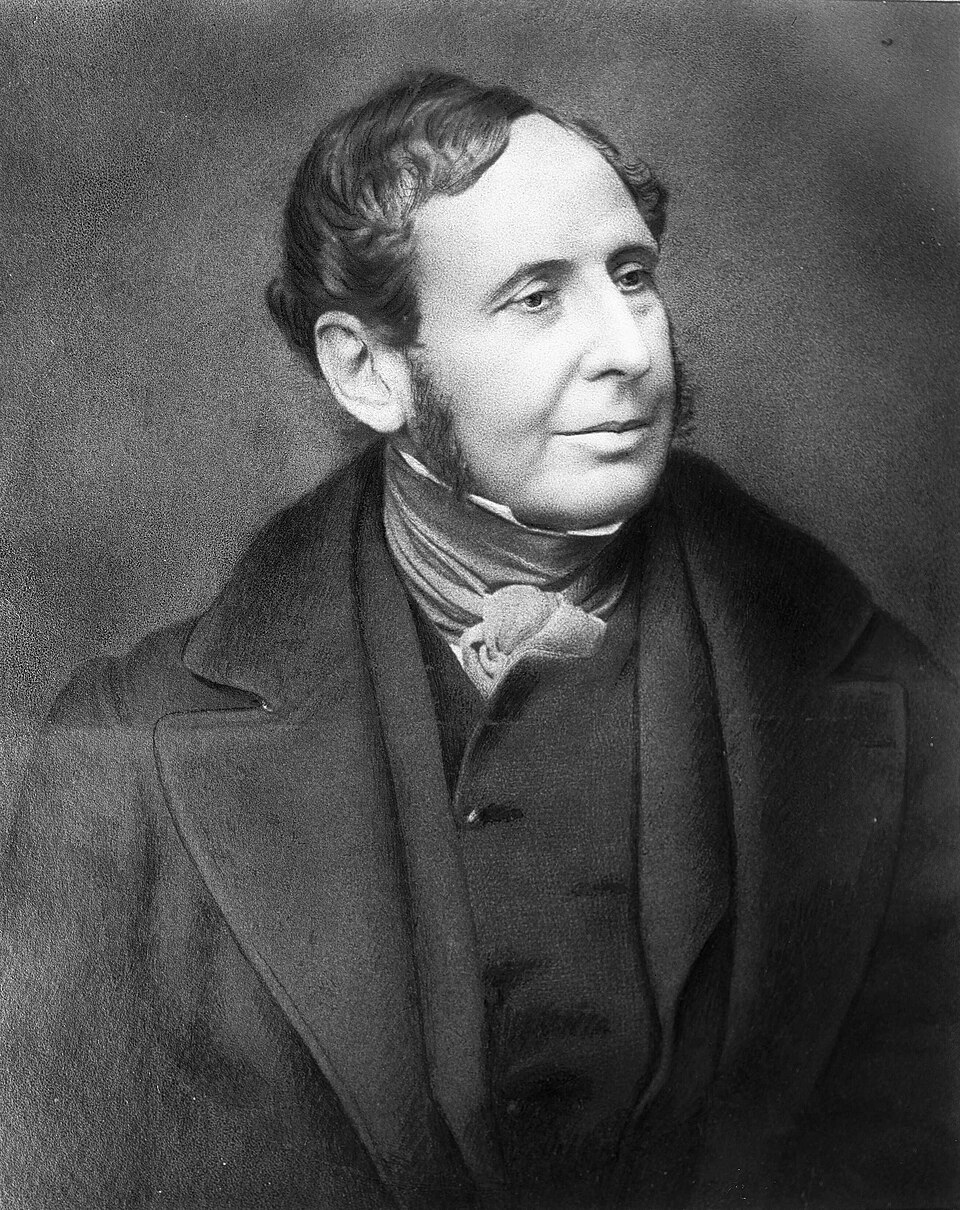
\includegraphics[height=0.27\textheight]{ch1_fitzroy_1910.jpg}\\[1mm]
\imgcap{Robert FitzRoy (1805--1865)}
\imgcredit{https://commons.wikimedia.org/wiki/File:Robert_Fitzroy.jpg}{Portret: Charles Hemus (c.\ 1910); domeniu public; Wikimedia Commons}\\[1mm]\centering
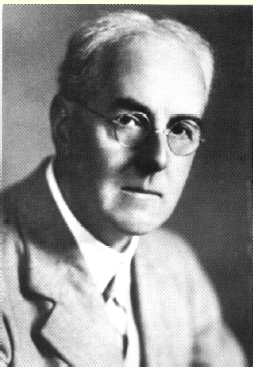
\includegraphics[height=0.22\textheight]{ch1_richardson.png}\\[1mm]
\imgcap{Lewis Fry Richardson (1881--1953)}
\imgcredit{https://commons.wikimedia.org/wiki/File:Lewis_Fry_Richardson.png}{Foto: NOAA; domeniu public; Wikimedia Commons}
\end{column}
\begin{column}{0.62\textwidth}
\begin{itemize}
    \item 1861: FitzRoy, conducătorul noului Meteorological Office, publică zilnic „prognoze” în The Times
    \begin{itemize}
        \item el a dat cuvîntului sensul modern; prognozele greșeau des și erau ironizate public
    \end{itemize}
    \item 1922: Richardson calculează o prognoză meteo prin integrarea numerică a ecuațiilor de mișcare, de mînă
    \item 1950: \refBrier\ propune un scor pentru prognozele probabilistice de ploaie; meteorologia conduce verificarea prognozelor în următorii cincizeci de ani
    \begin{itemize}
        \item economia adoptă aceleași instrumente tîrziu: PIT \refDGT, scoruri proprii \refGRa, calibrare \refGBR
    \end{itemize}
    \item Lecția: o prognoză este utilă doar în măsura în care știm să o evaluăm
\end{itemize}
\end{column}
\end{columns}
\end{frame}


%=============================================================================
\section{Prognoze punctuale și funcții de pierdere}
%=============================================================================

\begin{frame}{Cadrul și notațiile}
\itemsize{\small}
\begin{itemize}
    \item Ținta $Y_{t+h}$, mulțimea de informații $\mathcal{F}_t$, orizontul $h$; o \textbf{prognoză punctuală} $\hat y_{t+h|t}$ este măsurabilă în raport cu $\mathcal{F}_t$
    \begin{itemize}
        \item măsurabilă în raport cu $\mathcal{F}_t$: calculată doar din informația disponibilă la momentul $t$
        \item o \textbf{prognoză probabilistică} este o distribuție predictivă $F_{t+h|t}$ (densitate, cuantile, interval, ansamblu)
    \end{itemize}
    \item Plan în afara eșantionului: $R$ observații pentru estimare, $P$ prognoze pentru evaluare, $R + P + h - 1 = T$
    \begin{itemize}
        \item scheme: \textbf{fixă} (o singură estimare), \textbf{mobilă} (ultimele $R$), \textbf{recursivă} (tot trecutul); în \atschlink{https://danpele.github.io/Time-Series-Analysis/RO/Cursuri/capitol4_sezonalitate_prognoza.pdf}{TSA, Capitolul 4} aceasta este evaluarea cu origine mobilă
        \item $T$: eșantionul total; ultima prognoză, făcută la $R + P - 1$, are ținta $T$; schema contează pentru inferență: \refWest\ față de \refGW, secțiunea 4
    \end{itemize}
    \item Cunoscute din \atschlink{https://danpele.github.io/Time-Series-Analysis/RO/Cursuri/capitol0_introducere.pdf}{TSA, Capitolul 0}: MAE, RMSE, MAPE și MASE, independentă de scală \refHK
    \begin{itemize}
        \item $\mathrm{MAE} = P^{-1}\sum|e_t|$, $\mathrm{RMSE} = (P^{-1}\sum e_t^2)^{1/2}$, $\mathrm{MAPE} = 100P^{-1}\sum|e_t/y_t|$; MASE: MAE împărțit la MAE-ul în eșantion al prognozei naive
        \item aici întrebarea este alta: \emph{ce} pierdere și ce răsplătește ea?
    \end{itemize}
\end{itemize}
\end{frame}

\begin{frame}{Prognoza punctuală optimă și consistența (1/2)}
\itemsize{\small}
\begin{itemize}
    \item Dată o pierdere $L(x, y)$ și o distribuție predictivă $F$, prognoza \textbf{optimă} (Bayes) minimizează pierderea așteptată:
    \begin{itemize}
        \item $x^* = \arg\min_x \E_F[L(x, Y)]$
        \item $x$: prognoza punctuală; $y$: realizarea; $L(x, y) \ge 0$: penalizarea; $\E_F$: media calculată cînd $Y \sim F$
    \end{itemize}
    \item O \textbf{funcțională} $\mathrm{T}(F)$ asociază unei distribuții un număr: media, mediana, o cuantilă
    \begin{itemize}
        \item $L$ este \textbf{consistentă} pentru $\mathrm{T}$ dacă $\E_F L(\mathrm{T}(F), Y) \le \E_F L(x, Y)$ pentru orice $x$ și $F$ \refGnaa
        \item adică raportarea lui $\mathrm{T}(F)$ este optimă oricare ar fi $F$; consistentă \textbf{strict}: egalitate doar pentru $x = \mathrm{T}(F)$
    \end{itemize}
\end{itemize}
\end{frame}

\begin{frame}{Prognoza punctuală optimă și consistența (2/2)}
\itemsize{\small}
\begin{itemize}
    \item Trei cazuri clasice, cu eroarea de prognoză $e = y - x$; anulăm derivata pierderii așteptate
    \begin{itemize}
        \item pătratică $e^2$: $\frac{d}{dx}\E(Y - x)^2 = -2\E(Y - x) = 0 \Rightarrow x^* = \E Y$ (media)
        \item absolută $|e|$: $\frac{d}{dx}\E|Y - x| = F(x) - (1 - F(x)) = 0 \Rightarrow F(x^*) = 1/2$ (mediana)
        \item pinball $\rho_\tau(e) = (\tau - \mathbf 1\{e < 0\})e$: $F(x) - \tau = 0 \Rightarrow x^* = F^{-1}(\tau)$ (cuantila $\tau$)
    \end{itemize}
    \item Notațiile pierderii pinball
    \begin{itemize}
        \item $\tau \in (0, 1)$: nivelul cuantilei; $\mathbf 1\{e < 0\}$: 1 dacă prognoza este prea mare, 0 altfel; $F^{-1}$: funcția cuantilă
        \item prognozele prea mici costă $\tau|e|$, cele prea mari $(1 - \tau)|e|$: un $\tau$ mare împinge prognoza în sus
    \end{itemize}
    \item Consecință: anunțați pierderea \emph{înainte} de a cere o prognoză; o prognoză-mediană judecată prin RMSE este judecată nedrept \refGnaa
\end{itemize}
\end{frame}

\begin{frame}{Trei pierderi, trei prognoze optime}
\itemsize{\footnotesize}
\begin{center}
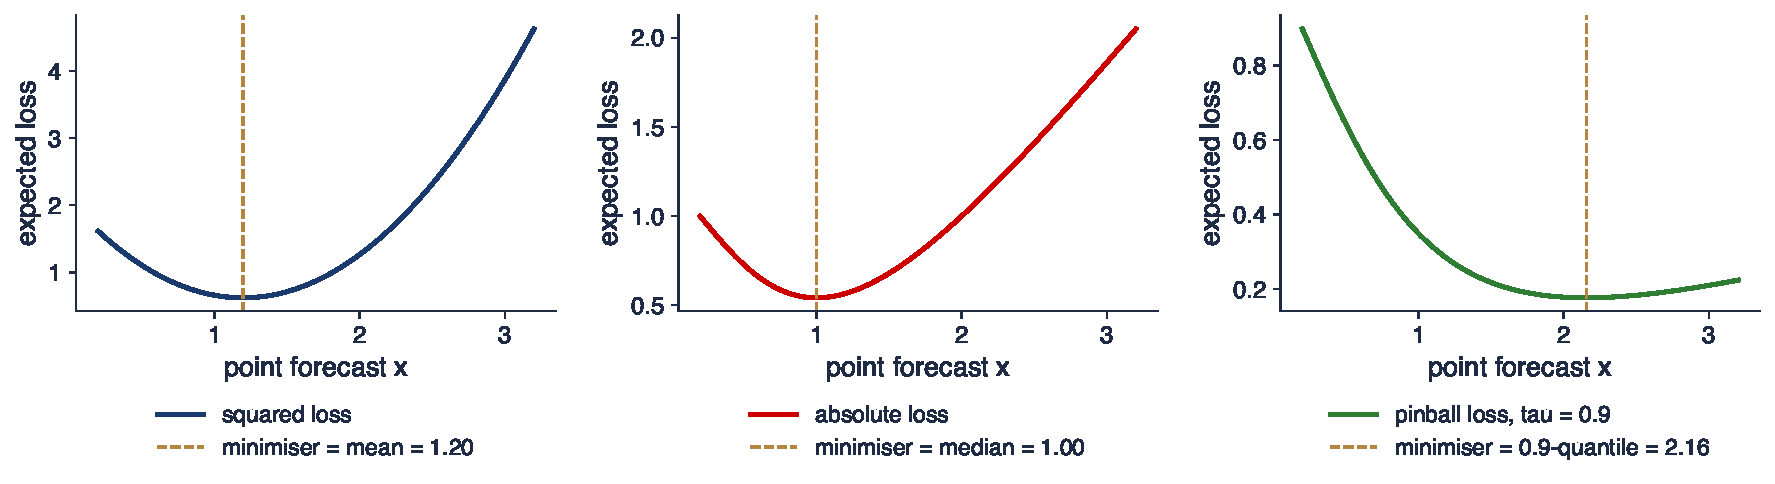
\includegraphics[width=0.97\textwidth,height=0.52\textheight,keepaspectratio]{ats_ch1_loss_minimizers.pdf}
\end{center}
\vspace{-0.25cm}
\begin{itemize}
    \item $Y$ log-normal cu $\ln Y \sim N(0, 0{,}6^2)$; pierderea așteptată ca funcție de prognoza punctuală $x$ (simulare, $2 \times 10^5$ extrageri)
\end{itemize}
\quantlet{ATS\_ch1\_loss\_functions}{\qlurl{ATS_ch1_loss_functions}}
\end{frame}

\begin{frame}{Interpretarea celor trei puncte de minim}
\itemsize{\small}
\begin{itemize}
    \item Media 1{,}20, mediana 1, cuantila de nivel 0,9: 2{,}16; trei prognoze „cele mai bune” diferite pentru aceeași variabilă
    \begin{itemize}
        \item pentru o țintă asimetrică la dreapta (salarii, consum de energie, prețuri, volatilitate) diferența este mare
    \end{itemize}
    \item Curba pinball este plată în jurul minimului: prognozele de cuantilă se deosebesc greu cu puține observații
    \item Un prognozator care cunoaște pierderea raportează funcționala potrivită; ierarhizarea cu altă pierdere răsplătește un comportament greșit
\end{itemize}
\end{frame}

\begin{frame}{Pierderile Bregman: toate pierderile consistente pentru medie (1/2)}
\itemsize{\small}
\begin{itemize}
    \item \textbf{Teoremă} \refSav, \refGnaa: în condiții de regularitate, $L$ este consistentă pentru medie dacă și numai dacă este o pierdere \textbf{Bregman}
    \begin{itemize}
        \item $L(x, y) = \phi(y) - \phi(x) - \phi'(x)(y - x)$
        \item $\phi$: o funcție convexă, $\phi'$ derivata ei; $L$ este distanța dintre $\phi(y)$ și tangenta la $\phi$ în $x$, deci $L \ge 0$ (pînă la termeni care depind doar de $y$)
    \end{itemize}
    \item Doi membri ai familiei
    \begin{itemize}
        \item $\phi(x) = x^2$: eroarea pătratică $(y - x)^2$
        \item $\phi(x) = -\ln x$: \textbf{QLIKE} $y/x - \ln(y/x) - 1$, pentru o prognoză de varianță $x > 0$ și un indicator al varianței $y > 0$ (\atschlink{https://danpele.github.io/Advanced-Time-Series/RO/Cursuri/capitol8_volatilitate_avansata.pdf}{Capitolul 8})
        \item media condiționată este optimă pentru orice pierdere Bregman \refBGW; demonstrația pentru cuantilă în \atsapplink{atsapp1}{atssrc1}{Anexă}
    \end{itemize}
\end{itemize}
\end{frame}

\begin{frame}{Pierderile Bregman: toate pierderile consistente pentru medie (2/2)}
\itemsize{\small}
\begin{itemize}
    \item Schița demonstrației, cu $\mu = \E Y$:
    \begin{itemize}
        \item $\E L(x, Y) - \E L(\mu, Y) = \phi(\mu) - \phi(x) - \phi'(x)(\mu - x) \ge 0$
        \item termenul liniar dispare deoarece $\E(Y - \mu) = 0$; inegalitatea este convexitatea lui $\phi$
    \end{itemize}
    \item Prognozele corect specificate se ierarhizează la fel sub orice pierdere Bregman; cele greșit specificate nu neapărat \refPatbz
    \begin{itemize}
        \item diagramele Murphy \refEGJK\ reprezintă scorul pe toată familia: o prognoză domină doar dacă este mai jos peste tot
        \item pentru volatilitate cu un indicator zgomotos, doar unele pierderi păstrează ierarhia \refPataa
    \end{itemize}
\end{itemize}
\end{frame}

\begin{frame}{Pierderi asimetrice}
\itemsize{\small}
\begin{itemize}
    \item Pierderea \textbf{LinEx} $L(e) = b[\exp(ae) - ae - 1]$, $e = y - x$: liniară de o parte, exponențială de cealaltă
    \begin{itemize}
        \item $b > 0$: o scală; $a$: asimetria; $a > 0$ penalizează exponențial prognozele prea mici ($e > 0$) și aproximativ liniar pe cele prea mari
        \item prognoza optimă $x^* = a^{-1}\ln\E e^{aY}$; cu $Y \mid \mathcal F_t \sim N(\mu_t, \sigma_t^2)$: $x^* = \mu_t + a\sigma^2_t/2$ \refCD
        \item prognoza optimă este \textbf{deplasată}, iar deplasarea se mișcă odată cu varianța condiționată
    \end{itemize}
    \item Consecințe pentru evaluare
    \begin{itemize}
        \item un prognozator rațional cu pierdere asimetrică pică testul MZ de nedeplasare (secțiunea 4)
        \item pierderea pinball este cazul liniar pe porțiuni: prognoza optimă este o cuantilă
    \end{itemize}
    \item Exemple: un operator de rețea (subestimarea consumului costă mai mult decît supraestimarea), o bancă centrală cu costuri asimetrice ale inflației, capitalul unei bănci (\atschlink{https://danpele.github.io/Advanced-Time-Series/RO/Cursuri/capitol9_var_es_backtesting.pdf}{Capitolul 9})
\end{itemize}
\end{frame}

\begin{frame}{Recapitulare: prognoze punctuale și funcții de pierdere}
\itemsize{\small}
\begin{itemize}
    \item Pierderea definește funcționala-țintă: pătratică $\to$ medie, absolută $\to$ mediană, pinball $\to$ cuantilă
    \item Pierderile Bregman sînt exact cele consistente pentru medie; QLIKE este una dintre ele
    \item Sub pierdere asimetrică prognoza optimă este deplasată prin construcție
    \item Cu modele greșit specificate ierarhia poate depinde de pierdere: fixați-o dinainte
\end{itemize}
\end{frame}


%=============================================================================
\section{Prognoze probabilistice: calibrare și sharpness}
%=============================================================================

\begin{frame}{Sharpness maxim sub condiția de calibrare}
\itemsize{\small}
\begin{itemize}
    \item \textbf{Calibrarea}: consistența statistică dintre prognozele $F_t$ și realizările $y_t$ (o proprietate comună a lor) \refGBR
    \begin{itemize}
        \item calibrare \textbf{probabilistică}: PIT (probability integral transform) $u_t = F_t(y_t)$, probabilitatea prognozată a unei realizări sub $y_t$, este în medie uniform
        \item calibrare \textbf{marginală}: $\frac1T\sum_t F_t(x) \to G(x)$ pentru orice $x$, cu $G$ limita distribuției empirice a lui $y_t$
    \end{itemize}
    \item \textbf{Sharpness}: concentrarea distribuțiilor predictive; o proprietate doar a prognozelor
    \begin{itemize}
        \item măsurată prin lățimea medie a intervalelor centrale sau prin varianța predictivă medie
    \end{itemize}
    \item Paradigma \refGBR: dintre prognozele calibrate, o preferăm pe cea mai concentrată
    \begin{itemize}
        \item prognoza climatologică (distribuția necondiționată) este calibrată, dar nu este concentrată
        \item scorurile proprii (secțiunea următoare) le răsplătesc pe amîndouă deodată
    \end{itemize}
\end{itemize}
\end{frame}

\begin{frame}{Transformarea integrală de probabilitate (PIT)}
\itemsize{\small}
\begin{itemize}
    \item \textbf{Teoremă} \refDawid, \refDGT: dacă $F_t$ este adevărata distribuție condiționată a lui $Y_t$ dată fiind $\mathcal{F}_{t-1}$ și este continuă, atunci $u_t = F_t(y_t)$ sînt i.i.d.\ $U(0, 1)$
    \begin{itemize}
        \item uniform: pentru orice $v \in (0,1)$, $P(u_t \le v \mid \mathcal{F}_{t-1}) = P(Y_t \le F_t^{-1}(v) \mid \mathcal F_{t-1}) = v$, oricare ar fi trecutul
        \item independent: o distribuție condiționată care nu depinde de trecut implică independența șirului
    \end{itemize}
    \item Pentru $h > 1$, valorile PIT sînt uniforme, dar dependente pînă la lagul $h - 1$ (orizonturi care se suprapun)
    \begin{itemize}
        \item testele trebuie să permită această dependență \refRS
    \end{itemize}
    \item Uniformitatea este necesară, nu suficientă: \refHamill\ și \refGBR\ construiesc prognozatori necalibrați al căror PIT este uniform în medie
    \begin{itemize}
        \item verificați PIT condiționat: pe subeșantioane, pe regimuri, pe orizonturi
    \end{itemize}
\end{itemize}
\end{frame}

\begin{frame}{Formele histogramelor PIT}
\itemsize{\footnotesize}
\begin{center}
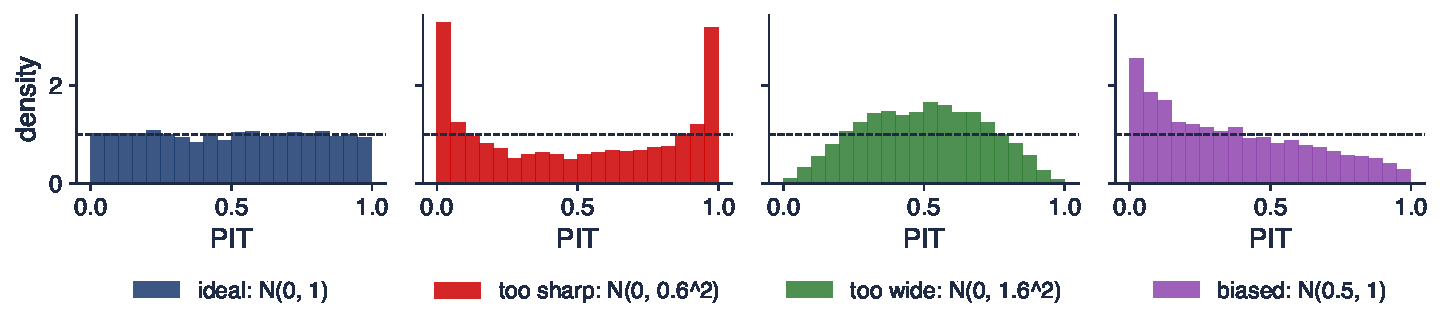
\includegraphics[width=0.97\textwidth,height=0.48\textheight,keepaspectratio]{ats_ch1_pit_shapes.pdf}
\end{center}
\vspace{-0.25cm}
\begin{itemize}
    \item $Y \sim N(0, 1)$, 5000 de extrageri; patru prognoze Normale; linia întreruptă: densitatea uniformă
\end{itemize}
\quantlet{ATS\_ch1\_calibration\_scores}{\qlurl{ATS_ch1_calibration_scores}}
\end{frame}

\begin{frame}{Interpretarea formelor PIT}
\itemsize{\small}
\begin{itemize}
    \item \textbf{Forma de U}: prea multe realizări în ambele cozi (32\% în afara intervalului central de 90\%, față de 10\%): prognoza este prea concentrată, intervalele prea înguste
    \item \textbf{Cocoașă}: prea puține realizări în cozi (1{,}0\%): prognoza este prea largă, intervalele risipesc informație
    \item \textbf{Pantă}: poziție deplasată; aici media prognozei este prea mare, deci valorile PIT se adună lîngă 0
    \item CRPS (mai mic este mai bine): ideală 0{,}567, prea concentrată 0{,}595, prea largă 0{,}604, deplasată 0{,}637: scorul propriu pune prognoza ideală pe primul loc
\end{itemize}
\end{frame}

\begin{frame}{Testarea calibrării (1/2)}
\itemsize{\small}
\begin{itemize}
    \item \textbf{Testul Berkowitz} \refBerk: dacă valorile PIT sînt i.i.d.\ uniforme, $z_t = \Phi^{-1}(u_t)$ este i.i.d.\ $N(0, 1)$
    \begin{itemize}
        \item $\Phi^{-1}$: funcția cuantilă a distribuției Normale standard
    \end{itemize}
    \item Estimăm un AR(1) gaussian pentru $z_t$ și îi testăm parametrii:
    \begin{itemize}
        \item $z_t = \mu + \rho(z_{t-1} - \mu) + \varepsilon_t$, $\quad \varepsilon_t \sim N(0, \sigma^2(1 - \rho^2))$
        \item $\mu$: media lui $z_t$; $\sigma^2$: varianța lui; $\rho$: autocorelația de ordinul întîi; calibrarea înseamnă $\mu = 0$, $\sigma = 1$, $\rho = 0$
        \item statistica LR (raportul de verosimilitate) $2(\ell_1 - \ell_0) \sim \chi^2(3)$ sub $H_0$; $\ell_1, \ell_0$: log-verosimilitățile maxime fără și cu restricții
        \item transformarea în $z$ face cozile vizibile; testul verifică doar primele două momente și dependența AR(1)
    \end{itemize}
\end{itemize}
\end{frame}

\begin{frame}{Testarea calibrării (2/2)}
\itemsize{\small}
\begin{itemize}
    \item \textbf{Corelogramele} lui $(u_t - \bar u)^k$, $k = 1, 2$ \refDGT: dependență în nivel și în volatilitate
    \begin{itemize}
        \item $\bar u$: media valorilor PIT; testul Ljung--Box pe $(u_t - \bar u)^2$ detectează dinamica de volatilitate omisă
    \end{itemize}
    \item Estimarea parametrilor schimbă distribuția sub ipoteza nulă a testelor PIT
    \begin{itemize}
        \item cu $P/R$ mic (puține prognoze față de eșantionul de estimare) efectul poate fi ignorat, altfel folosiți \refRS
    \end{itemize}
    \item Prognozele de interval: acoperirea și independența depășirilor \refChr
    \begin{itemize}
        \item depășire: o realizare în afara intervalului; pentru VaR aceasta devine backtesting (\atschlink{https://danpele.github.io/Advanced-Time-Series/RO/Cursuri/capitol9_var_es_backtesting.pdf}{Capitolul 9})
    \end{itemize}
\end{itemize}
\end{frame}

\begin{frame}{Studiu de caz: Diebold, Gunther și Tay (1998)}
\itemsize{\small}
\begin{itemize}
    \item Lucrarea: randamente zilnice S\&P 500; parametrii estimați o singură dată pe prima parte a eșantionului, prognozele de densitate evaluate pe partea a doua cu histograme PIT și corelograme ale lui $(u - \bar u)^k$ \refDGT
    \begin{itemize}
        \item modelele lor: i.i.d.\ Normal; MA(1)-GARCH(1,1) cu inovații Normale și cu inovații Student-$t$ \refBoll
    \end{itemize}
    \item Replicarea noastră: aceleași trei modele, estimate prin verosimilitate maximă pe 2000--2012, parametri ficși, prognoze de densitate la o zi pentru 2013--2026 ($3\,448$ zile)
    \begin{itemize}
        \item modelul: $r_t = c + \varepsilon_t + \theta\varepsilon_{t-1}$, $\varepsilon_t = \sigma_tz_t$, $\sigma_t^2 = \omega + \alpha\varepsilon_{t-1}^2 + \beta\sigma_{t-1}^2$; $z_t$ Normal sau Student-$t$ cu $\nu$ grade de libertate
        \item GARCH-$t$: $\hat\theta = \ensuremath{-}0{,}061$, $\hat\alpha + \hat\beta = 0{,}996$ (persistența volatilității), $\hat\nu = 8{,}0$ (cozi groase)
    \end{itemize}
    \item Întrebarea: care prognoză de densitate este calibrată și sînt de acord scorurile proprii cu diagnosticul PIT?
\end{itemize}
\end{frame}

\begin{frame}{Diagnosticul PIT pentru trei prognoze de densitate ale S\&P 500}
\itemsize{\footnotesize}
\begin{center}
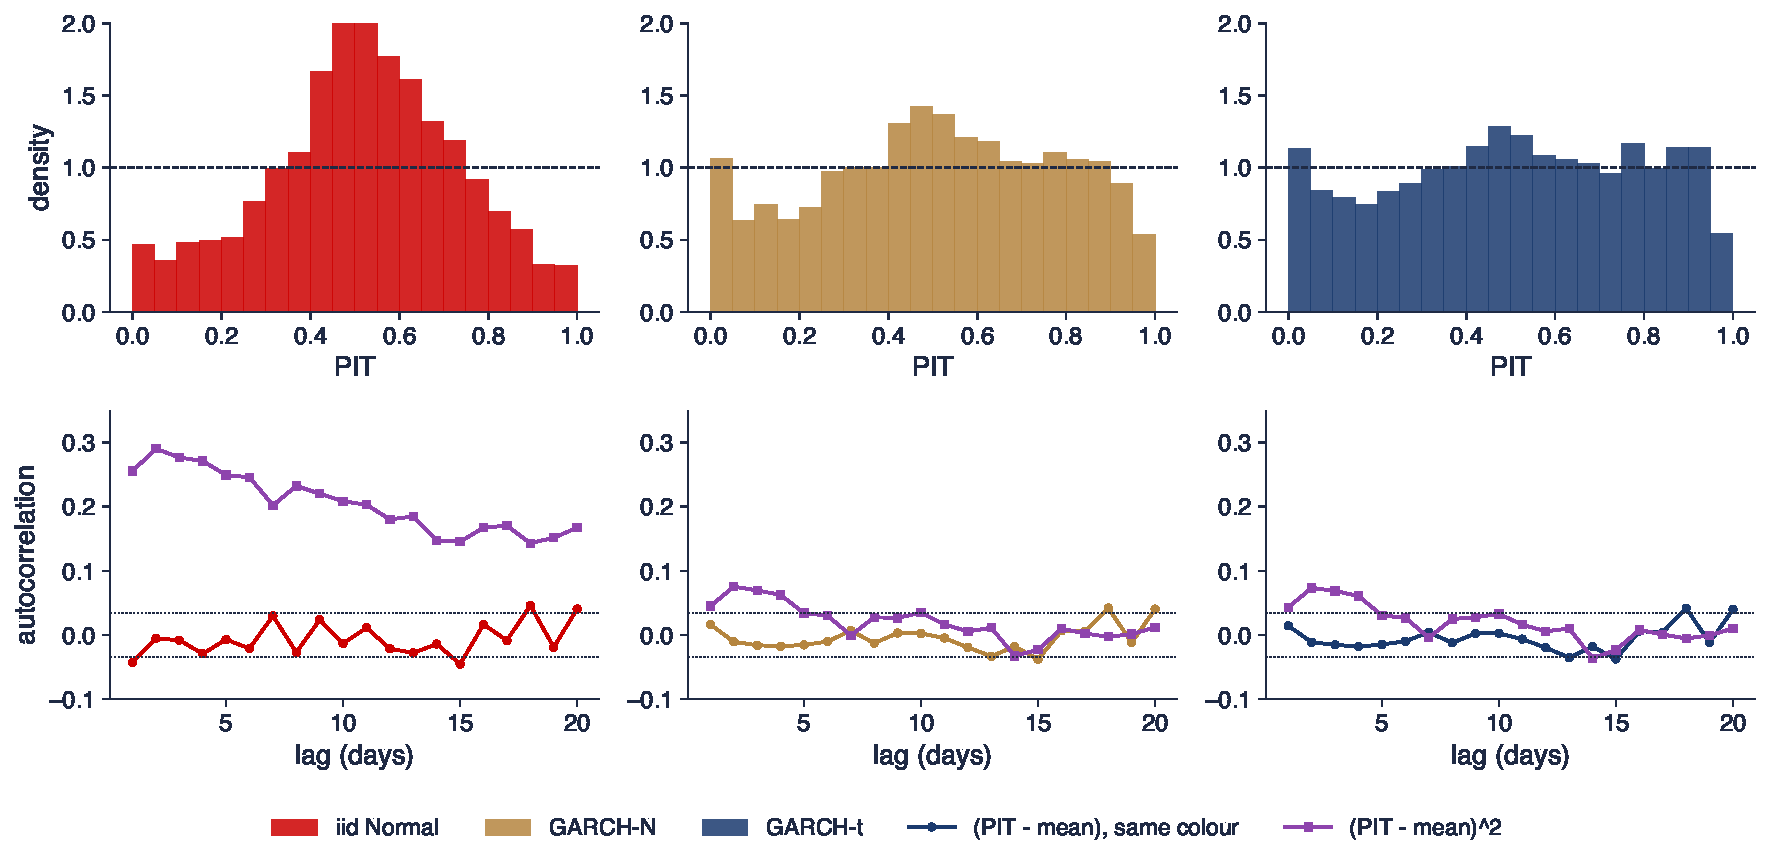
\includegraphics[width=0.97\textwidth,height=0.60\textheight,keepaspectratio]{ats_ch1_dgt.pdf}
\end{center}
\vspace{-0.25cm}
\begin{itemize}
    \item Sus: histograme PIT (20 de intervale); jos: autocorelațiile lui $(u - \bar u)$ și $(u - \bar u)^2$, cu benzile $\pm 2/\sqrt{T}$
\end{itemize}
\quantlet{ATS\_ch1\_density\_forecasts}{\qlurl{ATS_ch1_density_forecasts}}
\end{frame}

\begin{frame}{Interpretarea diagnosticului pentru S\&P 500}
\itemsize{\small}
\begin{itemize}
    \item i.i.d.\ Normal: o cocoașă și autocorelație puternică a lui $(u - \bar u)^2$: prognoza ignoră volatility clustering; Berkowitz LR 428{,}8 ($p$ $<$\,0{,}001)
    \begin{itemize}
        \item prea largă în perioadele calme, prea îngustă în cele agitate: cele două erori se compun într-o cocoașă
    \end{itemize}
    \item GARCH elimină cea mai mare parte a dependenței; varianta $t$ are o coadă stîngă mai bună
    \begin{itemize}
        \item Berkowitz: GARCH-N LR 9{,}3 ($p$ 0{,}026), GARCH-$t$ LR 10{,}0 ($p$ 0{,}019); $\sigma_z$ estimat 0{,}97 $< 1$
        \item în afara intervalului central de 90\%: 8{,}4\% din zile: cu parametri înghețați în 2012, prognozele sînt puțin prea largi după 2013
    \end{itemize}
    \item În acord cu \refDGT: heteroscedasticitatea condiționată este esențială, cozile groase ajută; rămîne o mică necalibrare reziduală
\end{itemize}
\end{frame}

\begin{frame}{Recapitulare: calibrarea}
\itemsize{\small}
\begin{itemize}
    \item Calibrarea este o proprietate comună a prognozelor și a realizărilor; sharpness este o proprietate a prognozelor
    \item Densitățile corecte la un pas dau valori PIT i.i.d.\ uniforme; pentru $h > 1$ ele sînt dependente
    \item Forma de U: prea concentrată; cocoașa: prea largă; panta: deplasare; corelograma lui $(u - \bar u)^2$: dinamica de volatilitate omisă
    \item S\&P 500: GARCH-$t$ este aproape calibrat, i.i.d.\ Normal nu este
\end{itemize}
\end{frame}


%=============================================================================
\section{Reguli de scor proprii și elicitabilitate}
%=============================================================================

\begin{frame}{Reguli de scor proprii}
\itemsize{\small}
\begin{itemize}
    \item O \textbf{regulă de scor} $S(F, y)$ atribuie o penalizare prognozei $F$ cînd se realizează $y$ (orientare negativă: mai mic este mai bine)
    \begin{itemize}
        \item \textbf{proprie}: $\E_G S(G, Y) \le \E_G S(F, Y)$ pentru orice $F, G$ \refGRa
        \item $G$: distribuția în care crede prognozatorul; $\E_G$: media sub $G$; raportarea convingerii adevărate este optimă
        \item \textbf{strict proprie}: egalitate doar dacă $F = G$; atunci scorul nu poate fi manipulat
    \end{itemize}
    \item Scorurile proprii răsplătesc calibrarea și sharpness împreună: scorul așteptat se descompune în incertitudine, minus rezoluție, plus fiabilitate
    \begin{itemize}
        \item scorul Brier $(p - \mathbf 1\{\text{eveniment}\})^2$, cu $p$ probabilitatea prognozată a unui eveniment binar, este cel mai vechi exemplu \refBrier
    \end{itemize}
    \item Un scor propriu al unei prognoze probabilistice devine o pierdere consistentă a unei prognoze punctuale cînd $F$ este o masă punctuală (CRPS $\to$ eroarea absolută)
\end{itemize}
\end{frame}

\begin{frame}{Scorul logaritmic}
\itemsize{\small}
\begin{itemize}
    \item $\mathrm{LogS}(f, y) = -\ln f(y)$ \refGood: singurul scor propriu \textbf{local} (depinde de $f$ doar în $y$, pînă la echivalență)
    \begin{itemize}
        \item $f$: densitatea prognozată; $g$: densitatea adevărată; caracterul propriu: $\E_g[\mathrm{LogS}(f, Y)] - \E_g[\mathrm{LogS}(g, Y)] = \int g \ln(g/f) = \mathrm{KL}(g \| f) \ge 0$
        \item $\mathrm{KL}$: divergența Kullback--Leibler, nenegativă și nulă doar dacă $f = g$ (inegalitatea Gibbs)
    \end{itemize}
    \item Legături: scorul logaritmic mediu = minus log-verosimilitatea în afara eșantionului; diferența a două scoruri logaritmice este un raport de verosimilitate predictivă
    \begin{itemize}
        \item factorii Bayes și alegerea predictivă a modelelor din \refGA\ se construiesc pe el
    \end{itemize}
    \item Slăbiciuni: infinit dacă $f(y) = 0$; foarte sensibil la evenimentele din coadă; cere o densitate
    \begin{itemize}
        \item nu poate evalua direct ansambluri sau prognoze de cuantile
    \end{itemize}
\end{itemize}
\end{frame}

\begin{frame}{Scorul probabilistic continuu (CRPS) (1/2)}
\itemsize{\small}
\begin{itemize}
    \item Definiția \refMW: distanța pătratică dintre funcția de repartiție prognozată și funcția treaptă a realizării
    \begin{itemize}
        \item $\mathrm{CRPS}(F, y) = \int_{-\infty}^{\infty}(F(z) - \mathbf 1\{y \le z\})^2dz$
        \item $z$: un prag; $\mathbf 1\{y \le z\}$: „funcția de repartiție” a realizării, 0 sub $y$ și 1 peste $y$; unitatea de măsură: cea a lui $y$
    \end{itemize}
    \item Forma cu nucleu \refGRa\ (demonstrația în \atsapplink{atsapp2}{atssrc2}{Anexă}):
    \begin{itemize}
        \item $\mathrm{CRPS}(F, y) = \E_F|X - y| - \frac12\E_F|X - X'|$, $\quad X, X' \sim F$ independente
        \item primul termen: acuratețea; al doilea: o recompensă pentru dispersie care împiedică scorul să favorizeze masele punctuale
        \item pentru o prognoză punctuală ($F$ masă punctuală în $x$) devine eroarea absolută $|y - x|$
    \end{itemize}
\end{itemize}
\end{frame}

\begin{frame}{Scorul probabilistic continuu (CRPS) (2/2)}
\itemsize{\small}
\begin{itemize}
    \item Forma închisă pentru $F = N(\mu, \sigma^2)$, cu $z = (y - \mu)/\sigma$:
    \begin{itemize}
        \item $\mathrm{CRPS} = \sigma\left[z(2\Phi(z) - 1) + 2\varphi(z) - 1/\sqrt\pi\right]$
        \item $\Phi$, $\varphi$: funcția de repartiție și densitatea lui $N(0,1)$; există o formă închisă și pentru Student $t$ (Quantlet)
        \item ansambluri: înlocuim $F$ cu distribuția empirică a membrilor
    \end{itemize}
    \item Descompuneri:
    \begin{itemize}
        \item $\mathrm{CRPS} = \int \mathrm{BS}_z\,dz = 2\int_0^1 \rho_\tau(y - F^{-1}(\tau))\,d\tau$
        \item $\mathrm{BS}_z$: scorul Brier al evenimentului $\{y \le z\}$; $\rho_\tau$: pierderea pinball la nivelul $\tau$
        \item deci media pinball pe cele 99 de percentile (GEFCom2014) aproximează CRPS/2 \refGEF
    \end{itemize}
\end{itemize}
\end{frame}

\begin{frame}{Scoruri pentru cuantile, intervale și vectori (1/2)}
\itemsize{\small}
\begin{itemize}
    \item \textbf{Scorul de cuantilă}: $\rho_\tau(y - q)$ pentru o prognoză $q$ a cuantilei $\tau$, strict consistent \refGnaa
    \begin{itemize}
        \item orice funcție crescătoare $g$ dă un alt scor consistent: $(\mathbf 1\{y \le q\} - \tau)(g(q) - g(y))$
    \end{itemize}
    \item \textbf{Scorul de interval} al unui interval central $(1 - \alpha)$, $[l, u]$ \refGRa
    \begin{itemize}
        \item $\mathrm{IS}_\alpha = (u - l) + \frac2\alpha(l - y)\mathbf 1\{y < l\} + \frac2\alpha(y - u)\mathbf 1\{y > u\}$
        \item $l, u$: limitele inferioară și superioară; lățimea plus o penalizare $2/\alpha$ pe unitatea de ratare
        \item este egal cu $\frac2\alpha[\rho_{\alpha/2}(y - l) + \rho_{1 - \alpha/2}(y - u)]$; acoperirea singură nu este un scor
    \end{itemize}
\end{itemize}
\end{frame}

\begin{frame}{Scoruri pentru cuantile, intervale și vectori (2/2)}
\itemsize{\small}
\begin{itemize}
    \item \textbf{Energy score} pentru vectori, CRPS multivariat:
    \begin{itemize}
        \item $\mathrm{ES}(F, \mathbf y) = \E\|\mathbf X - \mathbf y\| - \frac12\E\|\mathbf X - \mathbf X'\|$
        \item $\mathbf y$: vectorul realizărilor; $\mathbf X, \mathbf X'$: extrageri independente din prognoza $F$; $\|\cdot\|$: norma euclidiană
        \item slab în detectarea corelațiilor greșite; \textbf{variogram score} \refSH\ vizează structura de dependență (24 de consumuri orare, o traiectorie VAR)
        \item $\mathrm{VS}_p = \sum_{i,j}w_{ij}\big(|y_i - y_j|^p - \E|X_i - X_j|^p\big)^2$: compară diferențele observate și prognozate dintre componente; $w_{ij} \ge 0$: ponderi, $p$: de obicei 0,5
    \end{itemize}
    \item Cozile: CRPS ponderat pe praguri rămîne propriu \refGRjaa
    \begin{itemize}
        \item $\int (F(z) - \mathbf 1\{y \le z\})^2w(z)dz$
        \item $w(z) \ge 0$: o pondere care accentuează pragurile de interes (de exemplu coada stîngă); raportul de verosimilitate ponderat din \refAG\ nu rămîne propriu \refGRjaa
    \end{itemize}
\end{itemize}
\end{frame}

\begin{frame}{Scoruri proprii și improprii}
\itemsize{\footnotesize}
\begin{center}
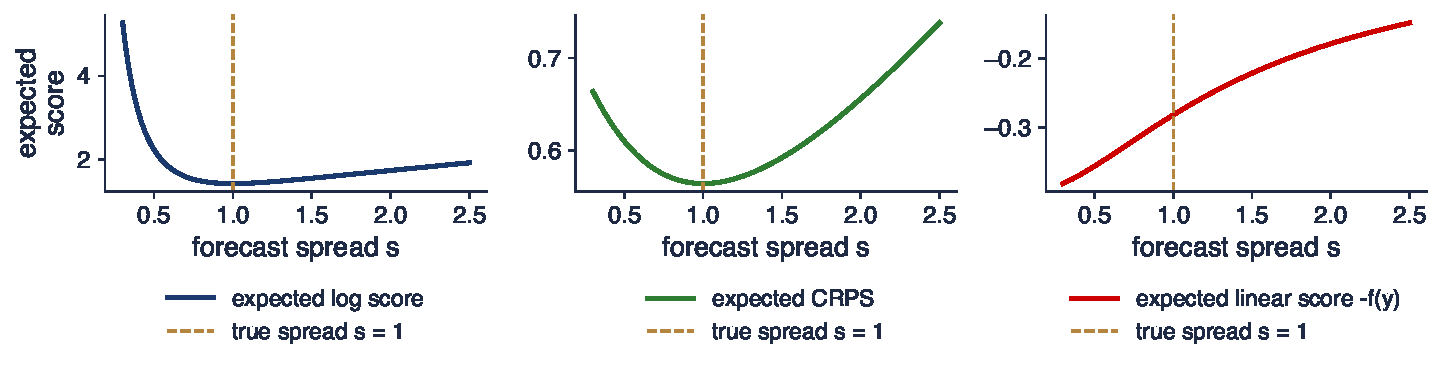
\includegraphics[width=0.97\textwidth,height=0.48\textheight,keepaspectratio]{ats_ch1_proper_scores.pdf}
\end{center}
\vspace{-0.25cm}
\begin{itemize}
    \item Adevărul $Y \sim N(0, 1)$; prognoza $N(0, s^2)$; scorul așteptat ca funcție de dispersia $s$ (forme închise)
    \item Scorul logaritmic și CRPS: minim la $s = 1$; scorul liniar $-f(y)$: $\E f(Y) = [2\pi(1 + s^2)]^{-1/2}$ crește cînd $s \to 0$: răsplătește excesul de încredere
\end{itemize}
\quantlet{ATS\_ch1\_calibration\_scores}{\qlurl{ATS_ch1_calibration_scores}}
\end{frame}

\begin{frame}{Interpretarea scorurilor așteptate}
\itemsize{\small}
\begin{itemize}
    \item Scorul logaritmic și CRPS sînt minime pentru dispersia adevărată: prognozatorul își maximizează recompensa așteptată raportînd ceea ce crede
    \item Scorul logaritmic penalizează excesul de încredere mult mai mult decît dispersia prea mare (ramura stîngă abruptă); CRPS este mai simetric și mărginit de eroarea absolută
    \item Scorul liniar este optimizat de o masă punctuală: ar răsplăti un prognozator care raportează mereu un vîrf, deci nu trebuie folosit la evaluare
\end{itemize}
\end{frame}

\begin{frame}{Elicitabilitate}
\itemsize{\small}
\begin{itemize}
    \item O funcțională $\mathrm T$ este \textbf{elicitabilă} dacă există o pierdere strict consistentă pentru ea \refGnaa
    \begin{itemize}
        \item media, cuantilele, expectilele, rapoartele de medii: elicitabile
        \item doar funcționalele elicitabile pot fi comparate și ierarhizate cu sens prin prognoze punctuale
    \end{itemize}
    \item \textbf{Condiție necesară} (Osband): mulțimi de nivel convexe: $\mathrm T(F_0) = \mathrm T(F_1) = t \Rightarrow \mathrm T(\lambda F_0 + (1 - \lambda)F_1) = t$
    \begin{itemize}
        \item $F_0, F_1$: două distribuții cu aceeași valoare $t$; $\lambda \in [0,1]$: ponderea mixturii
        \item \textbf{varianța} nu o îndeplinește, deci nu este elicitabilă; perechea (medie, al doilea moment) este
    \end{itemize}
    \item Măsurile de risc cu $\mathrm{VaR}_\alpha(X) = -q_\alpha(X)$, $q_\alpha$ cuantila de ordin $\alpha$ a randamentului $X$ (VaR 1\%: $\alpha = 0{,}01$)
    \begin{itemize}
        \item VaR este o cuantilă: elicitabil prin pierderea pinball
        \item ES (expected shortfall, pierderea medie dincolo de VaR) are mulțimi de nivel neconvexe: \textbf{nu este elicitabil} singur \refWeber, \refGnaa; perechea (VaR, ES) este elicitabilă \textbf{împreună} \refFZ
        \item funcțiile de scor Fissler--Ziegel și testele construite pe ele: \atschlink{https://danpele.github.io/Advanced-Time-Series/RO/Cursuri/capitol9_var_es_backtesting.pdf}{Capitolul 9}
    \end{itemize}
\end{itemize}
\end{frame}

\begin{frame}{Scorurile prognozelor de densitate pentru S\&P 500}
\itemsize{\footnotesize}
\begin{center}
\footnotesize
\begin{tabular}{lrrrr}
\toprule
\textbf{Model} & \textbf{Scor logaritmic} & \textbf{CRPS} & \textbf{În afara 90\%} & \textbf{Berkowitz $p$} \\
\midrule
i.i.d.\ Normal & 1{,}531 & 0{,}564 & 3{,}9\% & $<$\,0{,}001 \\
MA(1)-GARCH(1,1)-N & 1{,}265 & 0{,}509 & 8{,}0\% & 0{,}026 \\
MA(1)-GARCH(1,1)-$t$ & 1{,}233 & 0{,}507 & 8{,}4\% & 0{,}019 \\
\bottomrule
\end{tabular}
\end{center}
\begin{itemize}
    \item Diferențele de scor testate cu DM pe scorurile zilnice (\refAG, neponderat)
    \begin{itemize}
        \item GARCH-$t$ față de GARCH-N: HLN \ensuremath{-}5{,}9 (scor logaritmic), \ensuremath{-}6{,}4 (CRPS); GARCH-N față de i.i.d.: \ensuremath{-}12{,}7 și \ensuremath{-}21{,}5
    \end{itemize}
    \item Ambele scoruri ordonează modelele ca diagnosticul PIT; scorul logaritmic separă mai net cozile
    \item Ierarhizarea și calibrarea sînt întrebări diferite: modelul cu cel mai bun scor poate pica totuși un test de calibrare
\end{itemize}
\end{frame}

\begin{frame}{Recapitulare: scoruri proprii și elicitabilitate}
\itemsize{\small}
\begin{itemize}
    \item Scorurile proprii fac optimă raportarea sinceră; cele strict proprii nu pot fi manipulate
    \item LogS: local, sensibil la cozi; CRPS: robust, merge pentru ansambluri, egal cu dublul pierderii pinball integrate
    \item Scorul de interval pentru intervale, energy și variogram score pentru vectori
    \item Elicitabile: media, cuantila (VaR); neelicitabile: varianța, ES singur; (VaR, ES) împreună
\end{itemize}
\end{frame}


%=============================================================================
\section{Compararea prognozelor}
%=============================================================================

\begin{frame}{Două întrebări despre capacitatea predictivă}
\itemsize{\small}
\begin{itemize}
    \item \textbf{Populație} \refWest: sînt \emph{modelele}, la parametrii lor pseudo-adevărați, la fel de precise?
    \begin{itemize}
        \item eroarea de estimare intră în varianța asimptotică, cu excepția cazului $P/R \to 0$ sau cînd pierderea este cea folosită la estimare
    \end{itemize}
    \item \textbf{Eșantion finit} \refGW: sînt \emph{metodele de prognoză}, cu ferestrele lor de estimare, la fel de precise?
    \begin{itemize}
        \item fereastră mobilă de dimensiune fixă $R$: zgomotul de estimare face parte din metodă; modelele imbricate sînt permise
    \end{itemize}
    \item \textbf{Diebold--Mariano} \refDM\ tratează prognozele ca date („primitive”): compară prognoze, nu modele \refDie
    \begin{itemize}
        \item folosirea DM pentru a compara modele cu parametri estimați cere cadrul West sau GW
    \end{itemize}
\end{itemize}
\end{frame}

\begin{frame}{Testul Diebold--Mariano cu varianță HAC (1/2)}
\itemsize{\small}
\begin{itemize}
    \item Diferențialul de pierdere $d_t = L(e_{1t}) - L(e_{2t})$; $H_0$: $\E d_t = 0$ (acuratețe egală)
    \begin{itemize}
        \item $e_{it}$: eroarea prognozei $i$ la momentul $t$; $d_t > 0$: prognoza 2 a fost mai bună la $t$; presupunem $d_t$ staționar în covarianță
    \end{itemize}
    \item Statistica: diferențialul mediu împărțit la eroarea lui standard HAC
    \begin{itemize}
        \item $\mathrm{DM} = \bar d/\sqrt{\hat\sigma^2_{LR}/P} \to N(0, 1)$, $\quad \sigma^2_{LR} = \gamma_0 + 2\sum_{k \ge 1}\gamma_k$
        \item $\bar d$: media lui $d_t$ pe cele $P$ prognoze; $\gamma_k$: autocovarianțele lui $d_t$; $\sigma^2_{LR}$: varianța lui de termen lung (\atschlink{https://danpele.github.io/Advanced-Time-Series/RO/Cursuri/capitol0_recapitulare_inferenta.pdf}{Capitolul 0})
        \item un DM mare și pozitiv: prognoza 2 este mai precisă; respingem la 5\% dacă $|\mathrm{DM}| > 1{,}96$
    \end{itemize}
\end{itemize}
\end{frame}

\begin{frame}{Testul Diebold--Mariano cu varianță HAC (2/2)}
\itemsize{\small}
\begin{itemize}
    \item Erorile optime la $h$ pași sînt cel mult MA($h - 1$), deci DM trunchiază la $h - 1$ laguri cu un nucleu \textbf{dreptunghiular}
    \begin{itemize}
        \item estimarea dreptunghiulară poate fi \textbf{negativă}; ponderile Newey--West (Bartlett) o păstrează pozitivă \refNW, cu prețul unei deplasări în jos
        \item prognozele suboptimale au erori cu memorie mai lungă: folosiți o lățime de bandă aleasă din date (\atschlink{https://danpele.github.io/Advanced-Time-Series/RO/Cursuri/capitol0_recapitulare_inferenta.pdf}{Capitolul 0})
    \end{itemize}
    \item \textbf{Corecția HLN} \refHLNig: o rescalare a lui DM pentru eșantioane mici
    \begin{itemize}
        \item $\mathrm{DM}^* = \mathrm{DM}\sqrt{(P + 1 - 2h + h(h - 1)/P)/P}$, comparat cu $t_{P-1}$
        \item factorul (sub 1) elimină deplasarea estimatorului varianței pentru erori MA($h - 1$); $t_{P-1}$: distribuția Student $t$ cu $P - 1$ grade de libertate, pentru $P$ mic
    \end{itemize}
\end{itemize}
\end{frame}

\begin{frame}{Mărimea testelor DM și HLN în eșantioane mici}
\itemsize{\footnotesize}
\begin{center}
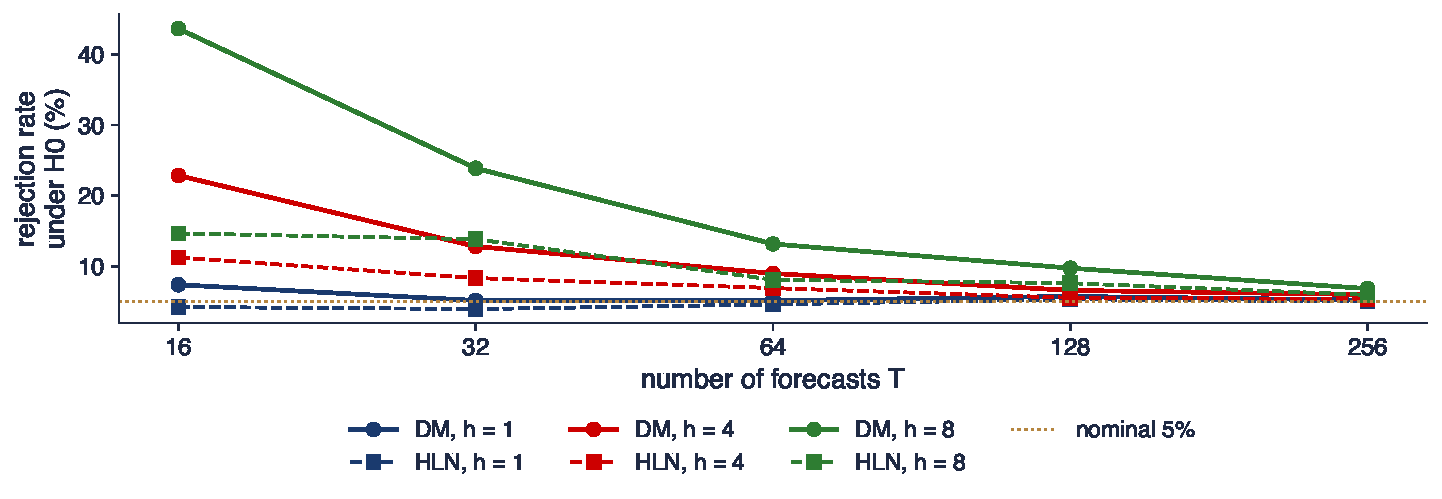
\includegraphics[width=0.97\textwidth,height=0.64\textheight,keepaspectratio]{ats_ch1_dm_size.pdf}
\end{center}
\vspace{-0.25cm}
\begin{itemize}
    \item Două serii de erori MA($h - 1$) independente, cu varianțe egale, pierdere pătratică; proporția respingerilor la 5\% în 4\,000 de replicări
\end{itemize}
\quantlet{ATS\_ch1\_dm\_tests}{\qlurl{ATS_ch1_dm_tests}}
\end{frame}

\begin{frame}{Interpretarea experimentului de mărime}
\itemsize{\small}
\begin{itemize}
    \item $h = 1$: ambele teste sînt aproape de 5\%; DM respinge prea des doar la $P = 16$ (7{,}4\%)
    \item $h = 8$, $P = 16$: DM respinge o ipoteză nulă adevărată în 43{,}6\% din cazuri, HLN în 14{,}6\%; la $P = 64$: 13{,}2\% și 8{,}1\%
    \begin{itemize}
        \item varianța HAC cu puține observații și multe laguri este zgomotoasă și deplasată în jos
    \end{itemize}
    \item Regulă: la orizonturi de mai mulți pași și cu mai puțin de aproximativ 100 de prognoze, folosiți HLN și tratați p-value-urile din jurul lui 5\% ca neconcludente; valorile critice fixed-$b$ (\atschlink{https://danpele.github.io/Advanced-Time-Series/RO/Cursuri/capitol0_recapitulare_inferenta.pdf}{Capitolul 0}) sînt o alternativă
\end{itemize}
\end{frame}

\begin{frame}{Inflația din România cu un an înainte: planul de evaluare}
\itemsize{\small}
\begin{itemize}
    \item Ținta: inflația IAPC, anuală, cu 12 luni înainte; originile prognozelor din ianuarie 2013, ținte de la ianuarie 2014 pînă în august 2026, $P = 152$ prognoze
    \begin{itemize}
        \item inflația IAPC în august 2026: 6{,}3\%
    \end{itemize}
    \item Prognozele
    \begin{itemize}
        \item \textbf{fără schimbare}: $\hat\pi_{t+12} = \pi_t$; \textbf{AR(3) direct}: $\pi_{t+12}$ pe $1, \pi_t, \pi_{t-1}, \pi_{t-2}$, OLS pe o fereastră mobilă de 10 ani
        \item \textbf{ținta}: ținta de inflație a BNR, 2,5\%; \textbf{media} dintre AR(3) și fără schimbare
    \end{itemize}
    \item Ținte de 12 luni care se suprapun: erorile sînt autocorelate pînă la lagul 11; DM cu $h = 12$
\end{itemize}
\end{frame}

\begin{frame}{Prognoze ale inflației din România cu un an înainte}
\itemsize{\footnotesize}
\begin{center}
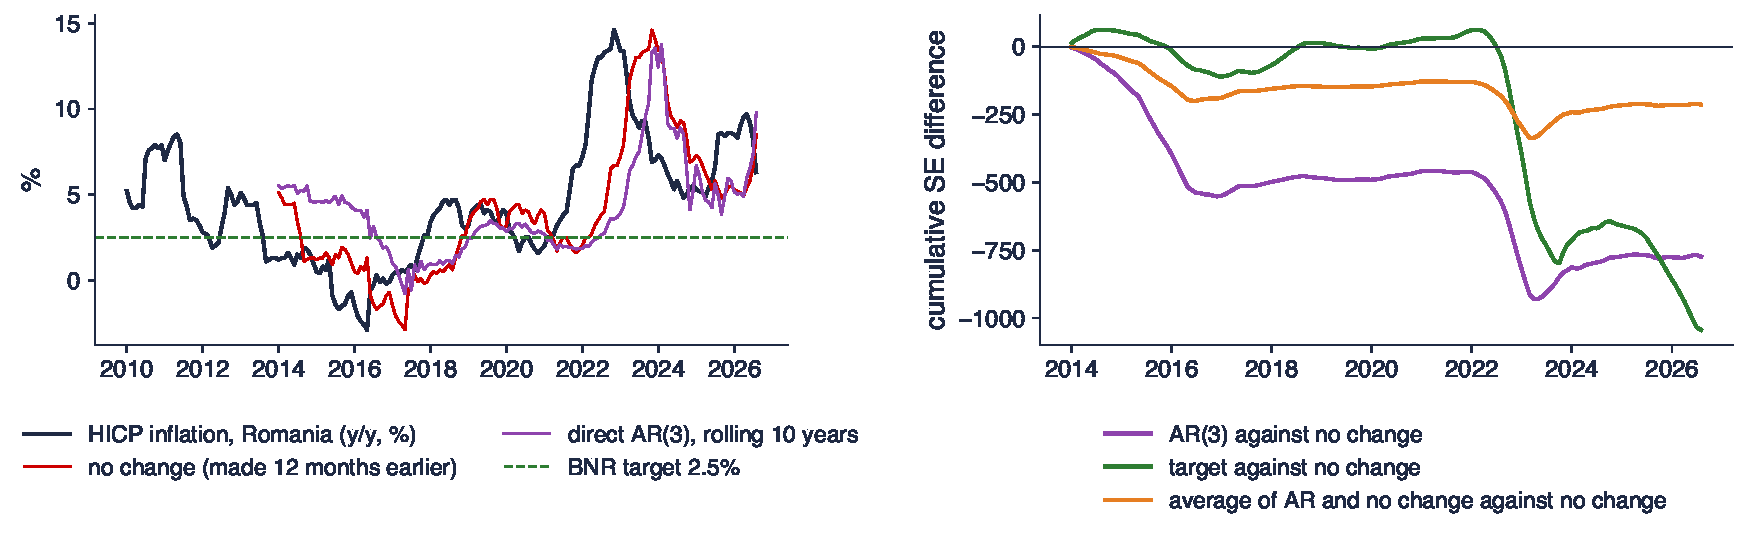
\includegraphics[width=0.97\textwidth,height=0.50\textheight,keepaspectratio]{ats_ch1_ro_inflation.pdf}
\end{center}
\vspace{-0.25cm}
\begin{itemize}
    \item Stînga: inflația și prognozele făcute cu 12 luni înainte; dreapta: suma cumulată a $e_{\mathrm{nc},t}^2 - e_{m,t}^2$ (scade: modelul $m$ pierde în fața prognozei fără schimbare)
\end{itemize}
\quantlet{ATS\_ch1\_dm\_tests}{\qlurl{ATS_ch1_dm_tests}}
\end{frame}

\begin{frame}{Interpretarea comparației pentru inflația din România}
\itemsize{\footnotesize}
\begin{center}
\footnotesize
\begin{tabular}{lrrrrr}
\toprule
\textbf{Prognoza} & \textbf{RMSE} & \textbf{DM} & \textbf{HLN} & \textbf{$p$ (HLN)} & \textbf{$p$, pierdere abs.} \\
\midrule
fără schimbare & 3{,}57 & -- & -- & -- & -- \\
AR(3) & 4{,}23 & 1{,}43 & 1{,}32 & 0{,}188 & 0{,}381 \\
ținta BNR & 4{,}43 & 1{,}30 & 1{,}21 & 0{,}230 & 0{,}319 \\
media & 3{,}76 & 0{,}96 & 0{,}88 & 0{,}378 & 0{,}795 \\
\bottomrule
\end{tabular}
\end{center}
\begin{itemize}
    \item Fiecare model are RMSE mai mare decît prognoza fără schimbare, totuși nicio diferență nu este semnificativă: cu $P = 152$ ținte suprapuse, eșantionul efectiv este mic
    \item Newey--West în locul nucleului dreptunghiular: HLN 1{,}47 pentru AR(3); concluzia nu depinde de nucleu
    \item RMSE relativ al AR(3): 1{,}44 înainte de iulie 2021, 1{,}10 după: ierarhia nu este stabilă în timp \refGRaz
\end{itemize}
\end{frame}

\begin{frame}{Capacitatea predictivă condiționată: Giacomini--White (1/2)}
\itemsize{\small}
\begin{itemize}
    \item $H_0$: $\E[d_{t+h} \mid \mathcal{G}_t] = 0$ \refGW
    \begin{itemize}
        \item $\mathcal{G}_t$: informația de la originea prognozei; $H_0$: niciun instrument $h_t \in \mathcal{G}_t$ nu prezice care metodă cîștigă
        \item $h_t$: un vector de $q$ instrumente (nu orizontul $h$), de exemplu o constantă și ultimul diferențial de pierdere
    \end{itemize}
    \item Statistica: un test Wald că instrumentele nu prezic $d_{t+h}$
    \begin{itemize}
        \item $\mathrm{GW} = P\,\bar Z'\hat\Omega^{-1}\bar Z \to \chi^2(q)$, $\quad Z_t = h_t d_{t+h}$
        \item $\bar Z$: media lui $Z_t$; $\hat\Omega$: matricea ei de covarianță HAC cu $h - 1$ laguri; $\chi^2(q)$: distribuția hi-pătrat cu $q$ grade de libertate
        \item $h_t = 1$ dă testul necondiționat; adăugînd $d_t$ sau o variabilă de stare testăm dacă trecutul prezice cîștigătorul
    \end{itemize}
\end{itemize}
\end{frame}

\begin{frame}{Capacitatea predictivă condiționată: Giacomini--White (2/2)}
\itemsize{\small}
\begin{itemize}
    \item Valid cu o fereastră \textbf{mobilă} de dimensiune fixă, modele imbricate sau nu, orice pierdere; nevalid cu o fereastră recursivă
    \begin{itemize}
        \item o respingere sugerează o regulă de decizie: folosiți modelul 1 cînd $\hat\delta'h_t > 0$, cu $\hat\delta$ coeficienții regresiei lui $d_{t+h}$ pe $h_t$
    \end{itemize}
    \item Inflația din România, AR(3) față de fără schimbare, $h_t = (1, d_t, \pi_t - 2{,}5)$
    \begin{itemize}
        \item $\pi_t - 2{,}5$: distanța inflației față de ținta BNR
        \item $\mathrm{GW} = 3{,}19$, p-value 0{,}363: nici pierderea recentă, nici distanța față de țintă nu prezic cîștigătorul
    \end{itemize}
\end{itemize}
\end{frame}

\begin{frame}{Modele imbricate: eșecul testului DM și testul Clark--West (1/2)}
\itemsize{\small}
\begin{itemize}
    \item Modelul 1 (mic, de exemplu mersul aleator) este imbricat în modelul 2; sub $H_0$ coeficienții suplimentari sînt nuli
    \begin{itemize}
        \item MSPE: eroarea medie pătratică de prognoză; în populație, MSPE-urile sînt egale, iar $d_t$ este degenerat
        \item de aceea statistica DM nu este asimptotic Normală \refCM
    \end{itemize}
    \item În eșantion finit, modelul 2 estimează cu zgomot niște coeficienți nuli
    \begin{itemize}
        \item MSPE-ul lui este \textbf{mai mare} decît al modelului 1: DM respinge prea rar și are putere mică
    \end{itemize}
\end{itemize}
\end{frame}

\begin{frame}{Modele imbricate: eșecul testului DM și testul Clark--West (2/2)}
\itemsize{\small}
\begin{itemize}
    \item \textbf{Clark--West} \refCW: corectăm modelul mare pentru zgomotul pe care îl adaugă
    \begin{itemize}
        \item $f_t = e_{1t}^2 - [e_{2t}^2 - (\hat y_{1t} - \hat y_{2t})^2]$
        \item $e_{1t}, e_{2t}$: erorile modelului mic și ale celui mare; $\hat y_{1t}, \hat y_{2t}$: prognozele lor; diferența la pătrat dintre prognoze este zgomotul adăugat de modelul 2
        \item test $t$ unilateral pentru $\E f_t = 0$ față de $\E f_t > 0$ (modelul 2 mai bun), cu valori critice Normale
    \end{itemize}
    \item De ce funcționează corecția
    \begin{itemize}
        \item sub $H_0$, $\E e_1^2 - \E e_2^2 = -\E(\hat y_1 - \hat y_2)^2$: corecția recentrează diferențialul (\atsapplink{atsapp3}{atssrc3}{Anexă})
        \item aproximativ Normal pentru schemele mobile și recursive; valorile critice exacte din \refCM\ sînt nestandard
    \end{itemize}
\end{itemize}
\end{frame}

\begin{frame}{Studiu de caz: Meese și Rogoff pentru EUR/RON}
\itemsize{\small}
\begin{itemize}
    \item \refMR: modelele structurale ale cursului de schimb nu bat mersul aleator în afara eșantionului la orizonturi de pînă la un an
    \begin{itemize}
        \item planul lor: prognoze în afara eșantionului cu origine mobilă, RMSE față de mersul aleator; rezultatul a rezistat patruzeci de ani
    \end{itemize}
    \item Datele noastre: EUR/RON lunar (cursul de referință BNR, sfîrșitul lunii), $\Delta s_{t+1} = 100\Delta\ln S_{t+1}$; estimare recursivă, prognoze din ianuarie 2010 pînă în august 2026 ($P = 200$)
    \begin{itemize}
        \item $S_t$: cursul (lei pentru un euro); $\Delta s_{t+1}$: variația lui logaritmică lunară, în \%, pozitivă cînd leul se depreciază
        \item imbricate în mersul aleator ($\Delta\hat s = 0$): deriva, AR($p$), regresia UIP $\Delta s_{t+1} = a + b(i^{RO}_t - i^{ZE}_t)/12 + u$ \refFama
        \item $i^{RO}_t, i^{ZE}_t$: dobînzile la 3 luni, în \% pe an (împărțite la 12: pe lună); $a, b$: coeficienții regresiei
        \item fără parametri estimați: UIP impusă ($a = 0, b = 1$), momentum (media ultimelor trei variații)
    \end{itemize}
    \item UIP: paritatea neacoperită a dobînzilor, deprecierea așteptată este egală cu diferențialul de dobîndă
\end{itemize}
\end{frame}

\begin{frame}{EUR/RON: modele față de mersul aleator}
\itemsize{\footnotesize}
\begin{center}
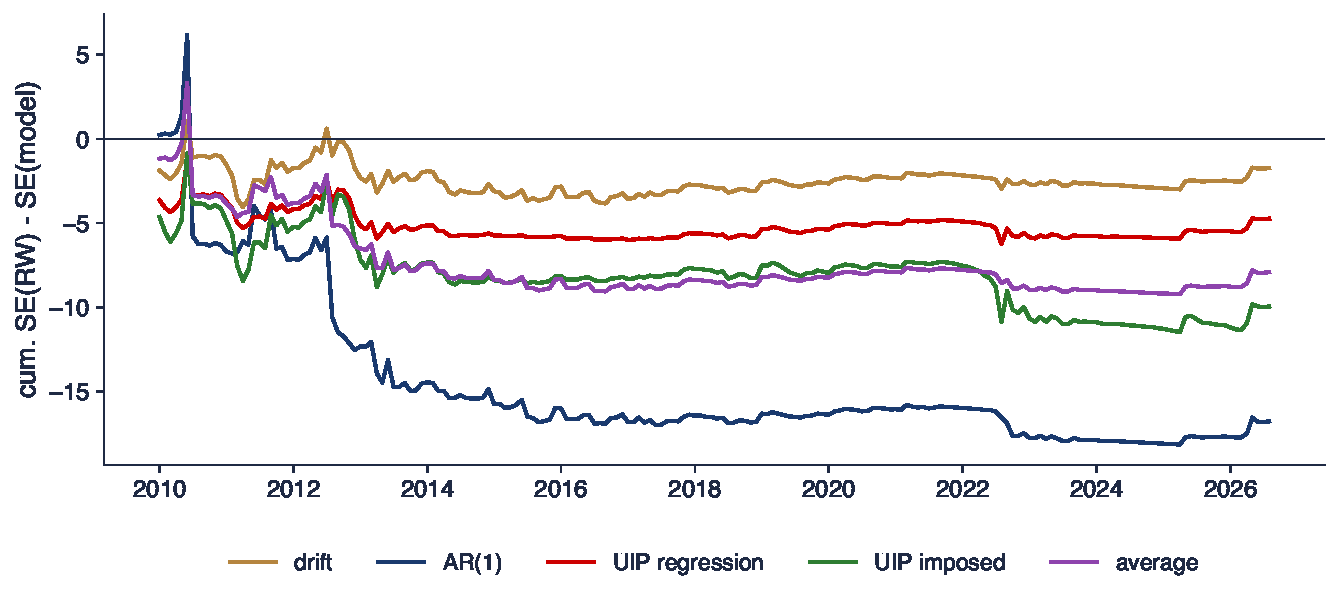
\includegraphics[width=0.97\textwidth,height=0.52\textheight,keepaspectratio]{ats_ch1_eurron.pdf}
\end{center}
\vspace{-0.25cm}
\begin{itemize}
    \item Suma cumulată $\sum_t(e^2_{RW,t} - e^2_{m,t})$ \refGWel: o linie sub zero arată că modelul $m$ a acumulat mai multă eroare pătratică decît mersul aleator
\end{itemize}
\quantlet{ATS\_ch1\_nested\_spa}{\qlurl{ATS_ch1_nested_spa}}
\end{frame}

\begin{frame}{Interpretarea testelor pentru EUR/RON}
\itemsize{\footnotesize}
\begin{center}
\scriptsize
\begin{tabular}{lrrrr}
\toprule
\textbf{Model} & \textbf{RMSE / RW} & \textbf{DM (HLN)} & \textbf{CW} & \textbf{$p$ (CW, unilateral)} \\
\midrule
deriva & 1{,}006 & 0{,}27 & 1{,}06 & 0{,}145 \\
AR(1) & 1{,}055 & 1{,}13 & \ensuremath{-}0{,}15 & 0{,}561 \\
AR(4) & 1{,}062 & 1{,}29 & \ensuremath{-}0{,}43 & 0{,}666 \\
regresia UIP & 1{,}016 & 0{,}76 & 0{,}10 & 0{,}458 \\
UIP impusă & 1{,}033 & 0{,}99 & -- & -- \\
momentum & 1{,}183 & 2{,}61 & -- & -- \\
media modelelor & 1{,}026 & 0{,}85 & -- & -- \\
\bottomrule
\end{tabular}
\end{center}
\begin{itemize}
    \item Toate modelele au RMSE mai mare decît mersul aleator (RMSE al mersului aleator: 0{,}86 puncte procentuale pe lună); rezultatul Meese--Rogoff se confirmă pentru leu
    \item Nici Clark--West nu respinge: corecția nu este suficientă pentru ca AR sau UIP să devină utile; doar deriva se apropie
    \item Managed float: BNR netezește cursul EUR/RON, deci variațiile lunare sînt mici și aproape imprevizibile cu acești predictori
\end{itemize}
\end{frame}

\begin{frame}{Raționalitate: Mincer--Zarnowitz și încadrarea (1/2)}
\itemsize{\small}
\begin{itemize}
    \item \textbf{Mincer--Zarnowitz} \refMZ: regresăm realizarea pe prognoză
    \begin{itemize}
        \item $y_{t+h} = a + b\hat y_{t+h|t} + u_{t+h}$
        \item sub pierdere pătratică o prognoză optimă are $(a, b) = (0, 1)$: fără deplasare, iar o variație cu o unitate a prognozei anunță o variație cu o unitate a realizării
        \item test Wald pentru $(a, b) = (0, 1)$ cu erori HAC ($u$ este MA($h - 1$)); $b < 1$: prognoze prea volatile; $b > 1$: prea timide
        \item versiunea extinsă: adăugăm variabile din $\mathcal{F}_t$; un coeficient semnificativ înseamnă informație nefolosită
    \end{itemize}
    \item MZ presupune pierdere pătratică: sub pierdere asimetrică o prognoză rațională este deplasată (secțiunea 1)
\end{itemize}
\end{frame}

\begin{frame}{Raționalitate: Mincer--Zarnowitz și încadrarea (2/2)}
\itemsize{\small}
\begin{itemize}
    \item \textbf{Încadrarea} \refChH, \refHLNih: prognoza 1 o încadrează pe prognoza 2 dacă 2 nu adaugă nimic la 1
    \begin{itemize}
        \item $y = (1 - \lambda)\hat y_1 + \lambda\hat y_2 + \varepsilon$, $\quad H_0$: $\lambda = 0$
        \item $\lambda$: ponderea prognozei 2 în cea mai bună combinație; $\lambda = 0$: prognoza 2 este inutilă dacă avem prognoza 1
        \item testul HLN: DM--HLN pe $d_t = e_{1t}(e_{1t} - e_{2t})$, unilateral ($\E d_t > 0$ înseamnă $\lambda > 0$)
    \end{itemize}
    \item Dacă niciuna nu o încadrează pe cealaltă, o combinație le bate pe amîndouă (secțiunea 5)
\end{itemize}
\end{frame}

\begin{frame}{Studiu de caz: Atkeson și Ohanian (2001)}
\itemsize{\small}
\begin{itemize}
    \item \refAO: o prognoză naivă, „inflația din următoarele patru trimestre este egală cu inflația din ultimele patru”, bate prognozele pe baza curbei Phillips în SUA după 1984
    \begin{itemize}
        \item curba Phillips din \refSWii: $\pi^4_{t+4} - \pi^4_t = a + \beta(L)u_t + \gamma(L)\Delta\pi_t + e_{t+4}$
        \item $\pi^4_t$: inflația pe ultimele patru trimestre; $\pi_t$: inflația trimestrială; $u_t$: rata șomajului; $\beta(L), \gamma(L)$: polinoame de laguri (cîte patru laguri)
    \end{itemize}
    \item Actualizarea noastră: IPC (media trimestrială) și rata șomajului (FRED); cîte patru laguri, fereastră mobilă de 15 ani; ținte din T1 1985 pînă în T2 2026 ($P = 166$)
    \begin{itemize}
        \item IPC pentru octombrie 2025 nu a fost publicat; media pentru T4 2025 folosește două luni
    \end{itemize}
    \item Teste: DM--HLN cu $h = 4$; GW cu $h_t = (1, d_t)$ și $h_t = (1, u_t)$; încadrare în ambele direcții
\end{itemize}
\end{frame}

\begin{frame}{Prognoza naivă față de curba Phillips}
\itemsize{\footnotesize}
\begin{center}
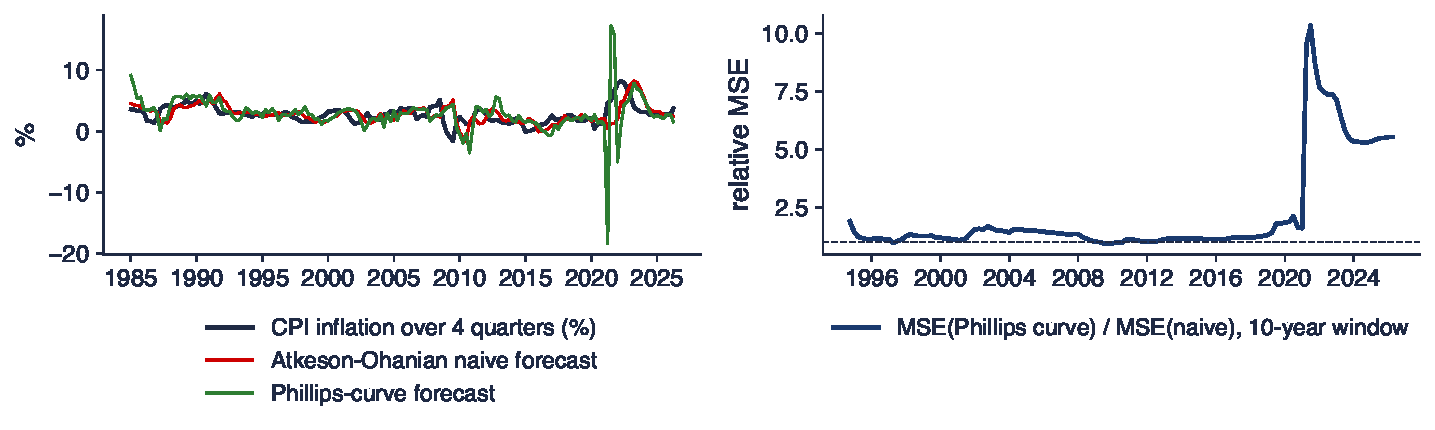
\includegraphics[width=0.97\textwidth,height=0.50\textheight,keepaspectratio]{ats_ch1_ao.pdf}
\end{center}
\vspace{-0.25cm}
\begin{itemize}
    \item Stînga: inflația IPC pe patru trimestre și cele două prognoze făcute cu patru trimestre înainte; dreapta: raportul MSE pe o fereastră mobilă de 10 ani
\end{itemize}
\quantlet{ATS\_ch1\_dm\_tests}{\qlurl{ATS_ch1_dm_tests}}
\end{frame}

\begin{frame}{Interpretarea actualizării Atkeson--Ohanian}
\itemsize{\small}
\begin{itemize}
    \item RMSE: naivă 1{,}69, curba Phillips 2{,}97 (raport 1{,}75); pe perioade: 1{,}29 (1985--2007), 1{,}10 (2008--2019), 2{,}38 (2020--2026)
    \item Totuși DM--HLN = 1{,}16, p-value 0{,}248: erorile mari de după 2020 măresc varianța HAC la fel de mult ca media
    \begin{itemize}
        \item raportul pe fereastră mobilă atinge 10{,}3 în T3 2021: curba Phillips a extrapolat saltul șomajului din pandemie
    \end{itemize}
    \item GW: p-value 0{,}355 cu diferențialul din perioada anterioară, 0{,}322 cu șomajul
    \begin{itemize}
        \item încadrare, $H_0$ „prognoza naivă încadrează curba Phillips”: p-value 0{,}289
        \item încadrare, $H_0$ „curba Phillips încadrează prognoza naivă”: p-value 0{,}118
    \end{itemize}
    \item Concluzia AO se păstrează în estimările punctuale, iar un test pe 41 de ani de date suprapuse nu le poate separa
\end{itemize}
\end{frame}

\begin{frame}{Multe modele: data snooping, reality check și SPA}
\itemsize{\small}
\begin{itemize}
    \item Testarea a $k$ modele față de un reper și raportarea celui mai mic p-value înseamnă \textbf{data snooping}
    \begin{itemize}
        \item $H_0$: $\max_{j \le k}\E[d_{j,t}] \le 0$ cu $d_{j,t} = L_{0,t} - L_{j,t}$: niciun model nu bate reperul
        \item $L_{0,t}$: pierderea reperului; $L_{j,t}$: pierderea modelului $j$; $d_{j,t} > 0$: modelul $j$ a fost mai bun la $t$
    \end{itemize}
    \item \textbf{Reality check} \refWhite: statistica $\max_j\sqrt P\bar d_j$, p-value-ul din bootstrap-ul staționar (\atschlink{https://danpele.github.io/Advanced-Time-Series/RO/Cursuri/capitol0_recapitulare_inferenta.pdf}{Capitolul 0}) sub configurația cea mai puțin favorabilă
    \begin{itemize}
        \item conservator: modelele foarte slabe deplasează în sus distribuția sub ipoteza nulă
    \end{itemize}
    \item \textbf{SPA} \refHan: studentizăm fiecare $\bar d_j$ și scoatem modelele clar inferioare din distribuția sub ipoteza nulă (p-value consistent)
    \begin{itemize}
        \item p-value-urile inferior și superior îl încadrează; cel superior este RC cu studentizare
        \item StepM \refRWze\ identifică \emph{care} modele bat reperul
    \end{itemize}
    \item EUR/RON, $k = 9$ modele față de mersul aleator: p-value SPA = 0{,}53 (inferior), 0{,}85 (consistent), 0{,}88 (superior): niciun model nu îl bate
\end{itemize}
\end{frame}

\begin{frame}{Mulțimea de încredere a modelelor (MCS) (1/2)}
\itemsize{\small}
\begin{itemize}
    \item \textbf{MCS} \refHLNaa: mulțimea $\hat{\mathcal M}_{1-\alpha}$ care conține cel mai bun model (sau modelele cele mai bune) cu probabilitatea de cel puțin $1 - \alpha$, asimptotic
    \begin{itemize}
        \item fără reper: toate modelele sînt tratate simetric; analog unui interval de încredere pentru un parametru
    \end{itemize}
    \item Testul de echivalență pentru cele $m$ modele rămase în mulțime
    \begin{itemize}
        \item $H_0$: $\E[d_{i\cdot,t}] = 0$ pentru orice $i$, $\quad d_{i\cdot,t} = L_{i,t} - \frac1m\sum_j L_{j,t}$
        \item $d_{i\cdot,t}$: pierderea modelului $i$ minus pierderea medie a tuturor modelelor; pozitiv: modelul $i$ este mai slab decît media
        \item statistica $T_{\max} = \max_i t_i$, $t_i = \bar d_{i\cdot}/\widehat{\mathrm{se}}(\bar d_{i\cdot})$: cel mai slab model față de medie, standardizat
    \end{itemize}
\end{itemize}
\end{frame}

\begin{frame}{Mulțimea de încredere a modelelor (MCS) (2/2)}
\itemsize{\small}
\begin{itemize}
    \item Algoritmul: pornim cu toate modelele
    \begin{itemize}
        \item dacă testul de echivalență respinge, \textbf{eliminăm} modelul cu cel mai mare $t_i$ și repetăm; ne oprim la prima nerespingere
        \item un bootstrap pe blocuri dă distribuția sub $H_0$ și erorile standard
        \item p-value-ul MCS al unui model: cel mai mare p-value al testelor pînă la eliminarea lui; modelul rămîne în $\hat{\mathcal M}_{1-\alpha}$ dacă acesta depășește $\alpha$
    \end{itemize}
    \item O mulțime MCS mare este și ea un rezultat
    \begin{itemize}
        \item datele nu pot separa modelele (un eșantion slab, nu modele egale)
    \end{itemize}
\end{itemize}
\end{frame}

\begin{frame}{Studiu de caz: consumul de electricitate din România pentru ziua următoare}
\itemsize{\footnotesize}
\begin{columns}[T]
\begin{column}{0.36\textwidth}
\centering
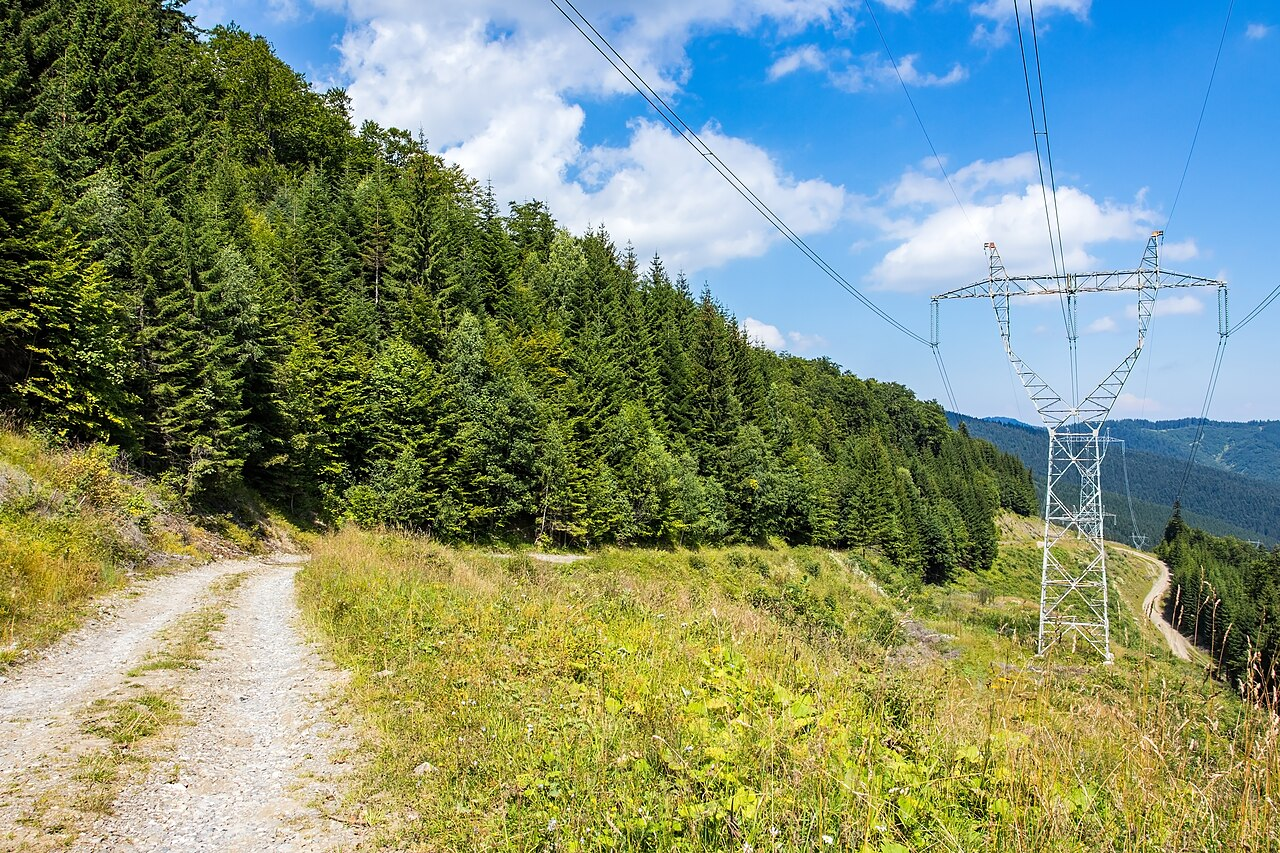
\includegraphics[height=0.36\textheight]{ch1_pylon_predelus_2018.jpg}\\[1mm]
\imgcap{O linie de 400 kV, Pasul Predeluș (2018)}
\imgcredit{https://commons.wikimedia.org/wiki/File:Delta_pylon_Pasul_Predelu\%C8\%99_RO_2018_-_1.jpg}{Foto: Drprv (2018); CC BY-SA 3.0; Wikimedia Commons}
\end{column}
\begin{column}{0.62\textwidth}
\begin{itemize}
    \item Ținta: cele 24 de consumuri orare ale zilei $d + 1$, cu date pînă în ziua $d$; 1 ianuarie 2025 -- 30 septembrie 2026 ($638$ zile); media 5{,}98 GW
    \begin{itemize}
        \item prognoze de cuantile la cele 99 de percentile, evaluate prin pierderea pinball medie ca în GEFCom2014 \refGEF, \refHF
    \end{itemize}
    \item Modele: naiv zi, naiv săptămînal, media pe 4 săptămîni; \textbf{ARX expert} din \refZW\ pentru fiecare oră
    \begin{itemize}
        \item regresori: $y_{d,h}, y_{d-1,h}, y_{d-6,h}$, minimul și maximul zilei $d$, ultima oră din $d$, luni, sîmbătă, duminică; fereastră mobilă de un an
        \item cuantile: prognoza punctuală plus cuantilele empirice ale ultimelor 182 de erori la aceeași oră
    \end{itemize}
    \item ARX: autoregresie cu variabile exogene (aici variabile calendaristice)
\end{itemize}
\end{column}
\end{columns}
\end{frame}

\begin{frame}{O săptămînă de iarnă cu prognoze de consum}
\itemsize{\footnotesize}
\begin{center}
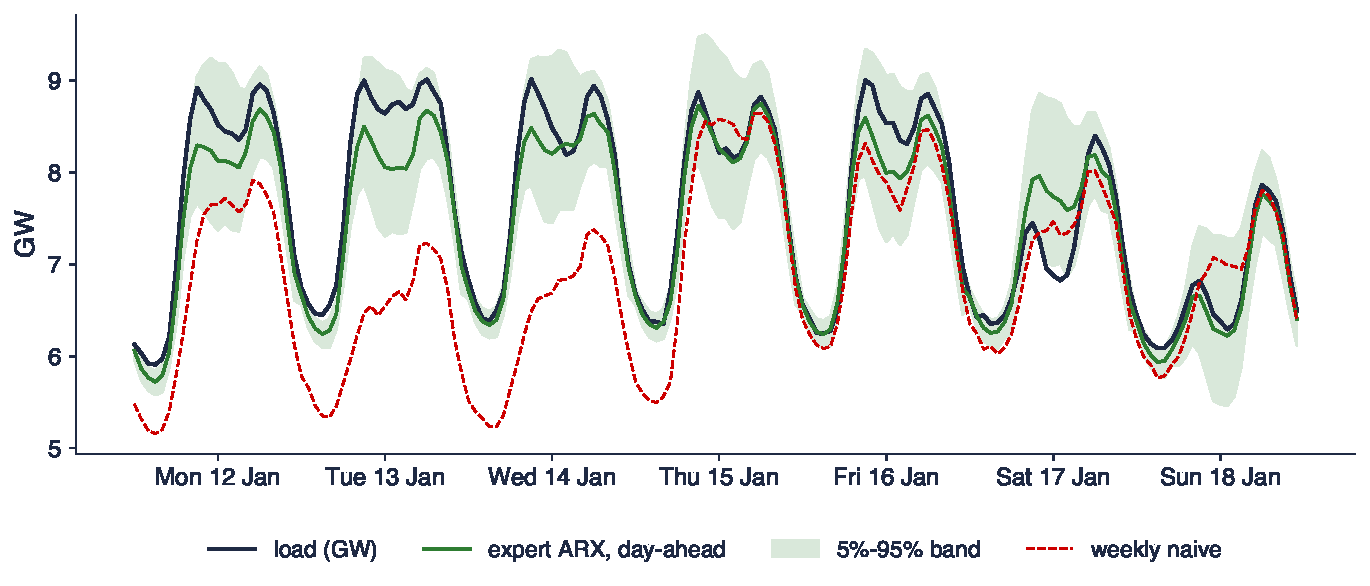
\includegraphics[width=0.97\textwidth,height=0.50\textheight,keepaspectratio]{ats_ch1_load_week.pdf}
\end{center}
\vspace{-0.25cm}
\begin{itemize}
    \item 12--18 ianuarie 2026; prognoza naivă săptămînală copiază săptămîna cu sărbători 5--9 ianuarie (Boboteaza și Sfîntul Ion, 6--7 ianuarie)
\end{itemize}
\quantlet{ATS\_ch1\_load\_mcs}{\qlurl{ATS_ch1_load_mcs}}
\end{frame}

\begin{frame}{Pierderea pinball medie și MCS de 90\%}
\itemsize{\footnotesize}
\begin{center}
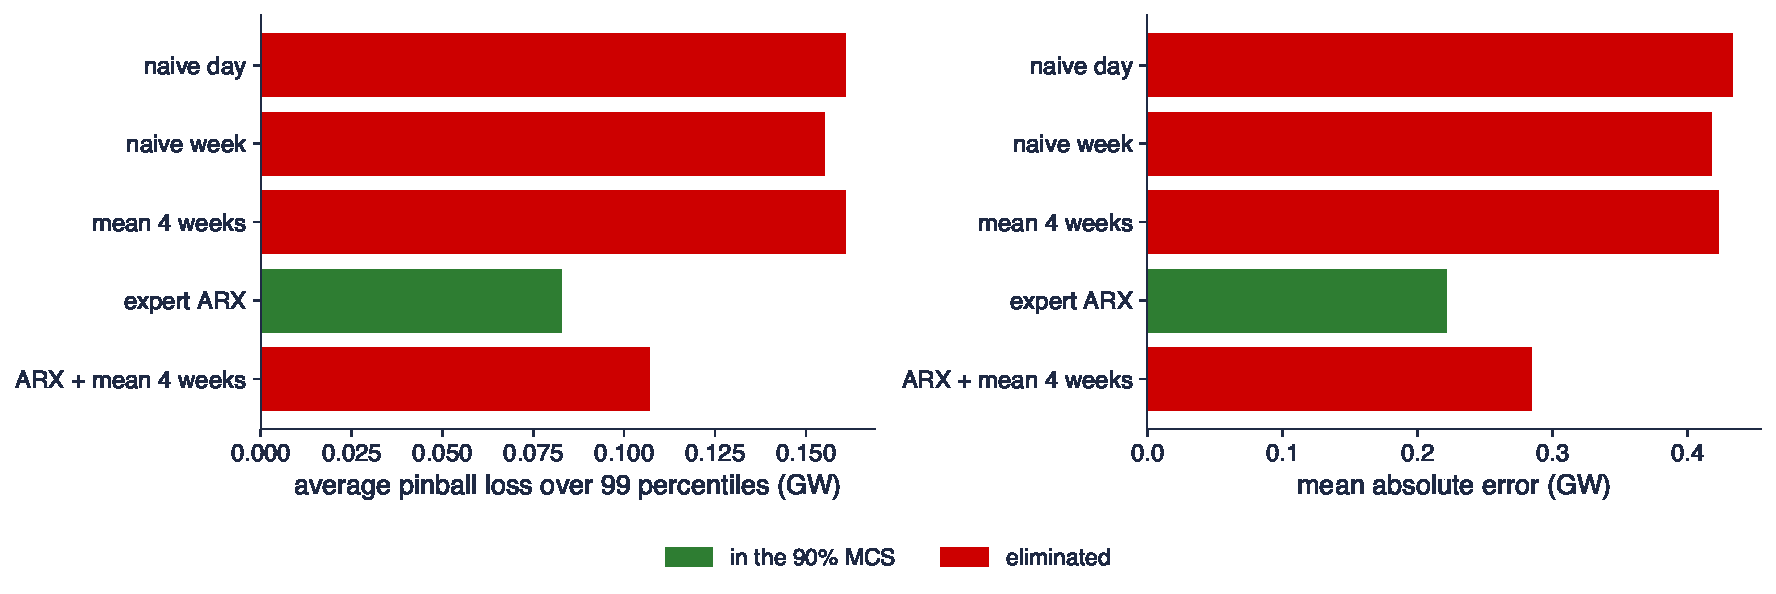
\includegraphics[width=0.97\textwidth,height=0.46\textheight,keepaspectratio]{ats_ch1_load_mcs.pdf}
\end{center}
\vspace{-0.25cm}
\begin{itemize}
    \item Pierderi medii zilnice; MCS cu $T_{\max}$, bootstrap pe blocuri mobile (blocuri de 7 zile), 2000 de replicări; verde: în MCS
\end{itemize}
\quantlet{ATS\_ch1\_load\_mcs}{\qlurl{ATS_ch1_load_mcs}}
\end{frame}

\begin{frame}{Interpretarea comparației pentru consumul de electricitate}
\itemsize{\footnotesize}
\begin{center}
\scriptsize
\begin{tabular}{lrrrr}
\toprule
\textbf{Model} & \textbf{Pinball (MW)} & \textbf{MAE (MW)} & \textbf{Acoperire 90\%} & \textbf{$p$ MCS} \\
\midrule
naiv (ziua $d$) & 161 & 433 & 89{,}2\% & $<$\,0{,}001 \\
naiv săptămînal & 155 & 417 & 87{,}6\% & $<$\,0{,}001 \\
media pe 4 săptămîni & 161 & 423 & 88{,}7\% & $<$\,0{,}001 \\
ARX expert & 83 & 221 & 88{,}2\% & 1{,}000 \\
ARX + media pe 4 săptămîni & 107 & 285 & 88{,}3\% & $<$\,0{,}001 \\
\bottomrule
\end{tabular}
\end{center}
\begin{itemize}
    \item ARX expert înjumătățește pierderile regulilor naive și este singur în MCS; DM--HLN față de combinația ARX + medie: \ensuremath{-}10{,}7
    \item Aici combinarea cu o prognoză mult mai slabă strică: ponderile egale ajută doar cînd prognozele au calitate asemănătoare (secțiunea 5)
    \item Toate intervalele acoperă puțin sub nivelul nominal; cele mai mari pierderi cad în zilele de sărbătoare legală și imediat după ele (8 ianuarie 2026, 25 decembrie 2025, 1 ianuarie 2025): efectele calendaristice sînt următoarea îmbunătățire
\end{itemize}
\end{frame}

\begin{frame}{Recapitulare: compararea prognozelor}
\itemsize{\small}
\begin{itemize}
    \item DM compară prognoze; pentru modele estimate alegeți West (populație) sau GW (metode, fereastră mobilă)
    \item Mai mulți pași, $P$ mic: varianță HAC plus corecția HLN și $t_{P-1}$
    \item Modele imbricate: Clark--West; multe modele: SPA sau MCS, niciodată cel mai mic p-value
    \item Inflația din România, inflația din SUA, EUR/RON: reperul simplu se bate greu, iar diferențele sînt rareori semnificative
\end{itemize}
\end{frame}


%=============================================================================
\section{Combinarea prognozelor}
%=============================================================================

\begin{frame}{Bates și Granger (1969)}
\itemsize{\footnotesize}
\begin{columns}[T]
\begin{column}{0.30\textwidth}
\centering
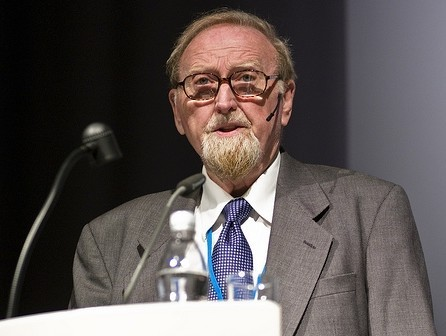
\includegraphics[height=0.32\textheight]{ch1_granger_2008.jpg}\\[1mm]
\imgcap{Clive W.~J.\ Granger (1934--2009), Premiul Nobel pentru Economie 2003}
\imgcredit{https://commons.wikimedia.org/wiki/File:Clive_Granger_by_Olaf_Storbeck.jpg}{Foto: Olaf Storbeck (2008); CC BY-SA 2.0; Wikimedia Commons}
\end{column}
\begin{column}{0.68\textwidth}
\begin{itemize}
    \item Două prognoze nedeplasate cu varianțele erorilor $\sigma_1^2, \sigma_2^2$ și covarianța $\sigma_{12}$; combinația $w\hat y_1 + (1 - w)\hat y_2$ \refBG
    \begin{itemize}
        \item varianța erorii $w^2\sigma_1^2 + (1 - w)^2\sigma_2^2 + 2w(1 - w)\sigma_{12}$, minimă pentru
        \item $w^* = \dfrac{\sigma_2^2 - \sigma_{12}}{\sigma_1^2 + \sigma_2^2 - 2\sigma_{12}}$, \quad $\sigma^2_c = \dfrac{\sigma_1^2\sigma_2^2 - \sigma_{12}^2}{\sigma_1^2 + \sigma_2^2 - 2\sigma_{12}} \le \min(\sigma_1^2, \sigma_2^2)$
        \item $\sigma^2_c$: varianța erorii combinației optime, niciodată peste cea a prognozei mai bune; prognoza mai puțin precisă primește ponderea mai mică
    \end{itemize}
    \item $N$ prognoze: $\mathbf w^* = \Sigma^{-1}\iota/(\iota'\Sigma^{-1}\iota)$, cu $\Sigma$ matricea de covarianță a erorilor și $\iota$ un vector de unu; \refGRm: regresia lui $y$ pe prognoze, cu sau fără termen liber și restricția ca ponderile să însumeze 1
    \begin{itemize}
        \item combinarea diversifică riscul de model, rupturile structurale și informația privată a prognozatorilor \refTim
    \end{itemize}
\end{itemize}
\end{column}
\end{columns}
\end{frame}

\begin{frame}{Paradoxul combinării prognozelor}
\itemsize{\small}
\begin{itemize}
    \item Regularitate empirică: media simplă bate ponderile „optime” estimate \refSWzd, \refTim, \refGKMT
    \begin{itemize}
        \item Stock--Watson: în 7 țări și cu mulți predictori ai creșterii economice, ponderile egale și mediana sînt printre cele mai bune combinații
    \end{itemize}
    \item \textbf{Explicația} \refSWal, \refCMVW: ponderile sînt estimate
    \begin{itemize}
        \item $\E[\mathrm{MSE}(\hat w)] = \mathrm{MSE}(w^*) + \E(\hat w - w^*)^2 D$, $D = \sigma_1^2 + \sigma_2^2 - 2\sigma_{12}$ (varianța lui $e_1 - e_2$)
        \item $\hat w$: ponderea estimată din $n$ erori trecute; MSE: eroarea pătratică medie a combinației
        \item cîștigul lui $w^*$ față de $1/2$: $(w^* - 1/2)^2D$; pierderea din estimare: $\mathrm{Var}(\hat w)D$, de ordinul $1/n$
        \item ponderile egale cîștigă cînd $(w^* - 1/2)^2 < \mathrm{Var}(\hat w)$: prognoze asemănătoare, eșantioane scurte, erori corelate
    \end{itemize}
    \item În plus: ponderile se schimbă la rupturi, deci ferestrele lungi sînt deplasate, iar cele scurte zgomotoase
\end{itemize}
\end{frame}

\begin{frame}{Paradoxul prin simulare}
\itemsize{\footnotesize}
\begin{center}
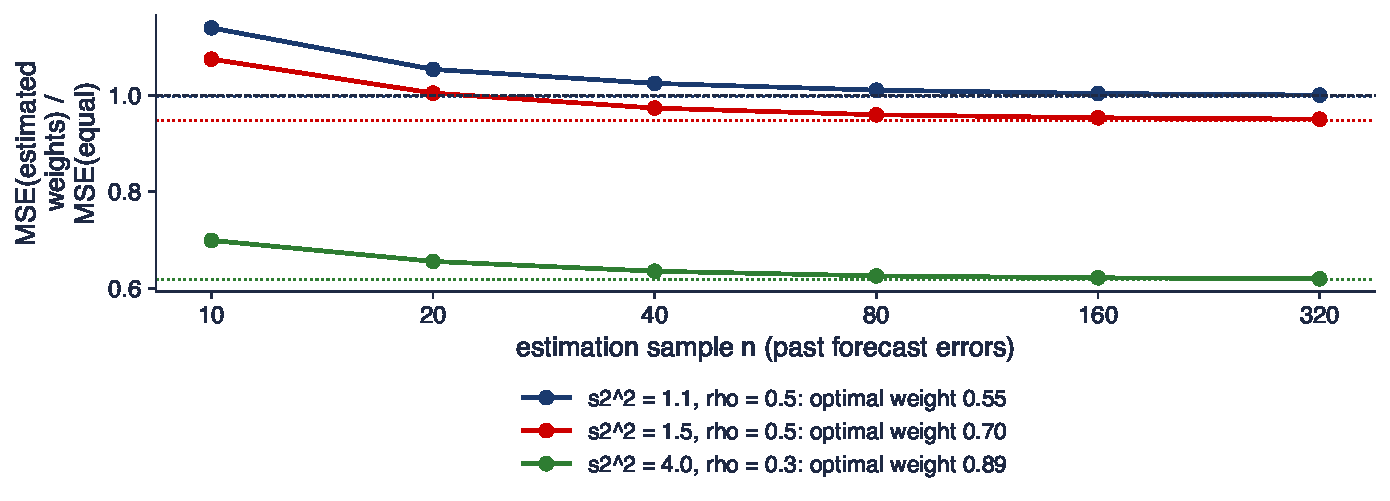
\includegraphics[width=0.97\textwidth,height=0.64\textheight,keepaspectratio]{ats_ch1_puzzle.pdf}
\end{center}
\vspace{-0.25cm}
\begin{itemize}
    \item Erori Normale bivariate cu $\sigma_1^2 = 1$; ponderi estimate din $n$ erori trecute; 4\,000 de replicări; punctat: raportul în populație $\mathrm{MSE}(w^*)/\mathrm{MSE}(1/2)$
\end{itemize}
\quantlet{ATS\_ch1\_combination}{\qlurl{ATS_ch1_combination}}
\end{frame}

\begin{frame}{Interpretarea simulării paradoxului}
\itemsize{\small}
\begin{itemize}
    \item Prognoze asemănătoare ($w^* = 0{,}55$): ponderea optimă reduce MSE-ul din populație doar la 0{,}997 din MSE-ul ponderilor egale, iar estimarea ei costă: raport 1{,}14 la $n = 10$, 1{,}024 la $n = 40$
    \item Moderat diferite ($w^* = 0{,}70$): ponderile estimate au nevoie de aproximativ 20 de erori trecute ca să nu piardă (1{,}07 la $n = 10$, 0{,}973 la $n = 40$)
    \item Foarte diferite ($w^* = 0{,}89$): estimați ponderile sau renunțați la prognoza slabă; cazul consumului de electricitate din secțiunea 4 este de acest tip
\end{itemize}
\end{frame}

\begin{frame}{Între ponderi egale și optime: shrinkage și combinări robuste}
\itemsize{\small}
\begin{itemize}
    \item \textbf{Shrinkage}: $\hat w_\lambda = \lambda\hat w + (1 - \lambda)\iota/N$ \refDP, \refSWzd
    \begin{itemize}
        \item $\hat w$: ponderile estimate; $\iota/N$: ponderi egale pentru $N$ prognoze; $\lambda \in [0,1]$: $\lambda = 0$ dă media, $\lambda = 1$ ponderile estimate
        \item un prior bayesian centrat pe ponderile egale; $\lambda$ scade cu numărul de prognoze și crește cu eșantionul
    \end{itemize}
    \item \textbf{Ponderi după performanță}: $w_i \propto 1/\mathrm{MSE}_i$ pe o fereastră recentă, ignorînd corelațiile; actualizarea dă erorilor recente o pondere mai mare
    \begin{itemize}
        \item \textbf{cel mai bun anterior}: alegem prognozatorul cu cel mai mic MSE trecut (o pondere egală cu 1)
    \end{itemize}
    \item \textbf{Robuste}: mediana, media trunchiată: protejează împotriva prognozatorilor extremi
    \item Panelurile de experți se schimbă: prognozatorii intră și ies, deci $\Sigma$ nu este niciodată observată complet \refCT
    \begin{itemize}
        \item ponderile după performanță cer un istoric minim; o sinteză a 50 de ani de practică: \refWHLK
    \end{itemize}
\end{itemize}
\end{frame}

\begin{frame}{Combinarea prognozelor de densitate}
\itemsize{\small}
\begin{itemize}
    \item \textbf{Combinarea liniară} (linear pool): $p(y) = \sum_i w_ip_i(y)$, $w_i \ge 0$, $\sum w_i = 1$ \refHM
    \begin{itemize}
        \item $p_i$: prognoza de densitate a modelului $i$; $w_i$: ponderea ei; combinarea este o mixtură de densități
        \item ponderile care minimizează scorul logaritmic mediu: \textbf{optimal prediction pools} \refGA
        \item ponderi interioare chiar dacă toate modelele sînt greșit specificate: o combinare nu este o medie de modele în sens bayesian
    \end{itemize}
    \item Combinarea liniară a unor densități calibrate este \textbf{supradispersată} \refGRjac
    \begin{itemize}
        \item mixtura adaugă varianța mediilor; remediul: o combinare transformată beta sau medierea cuantilelor (vincentizare)
    \end{itemize}
    \item Scorurile proprii (secțiunea 3) sînt criteriile naturale pentru estimarea și compararea combinărilor
\end{itemize}
\end{frame}

\begin{frame}{Combinări optime pentru densitățile S\&P 500}
\itemsize{\footnotesize}
\begin{center}
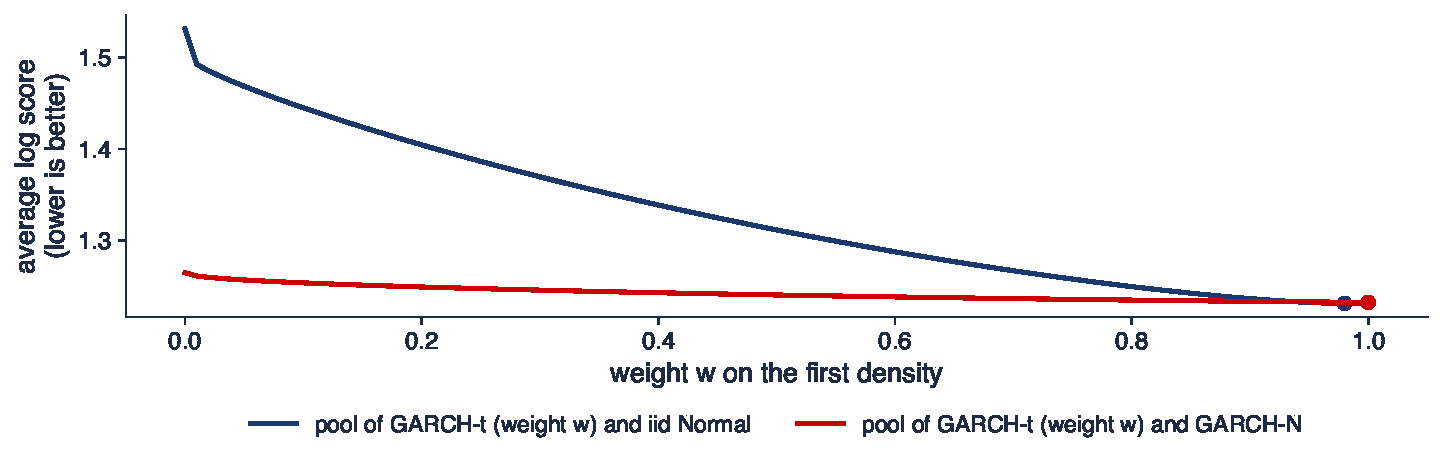
\includegraphics[width=0.97\textwidth,height=0.46\textheight,keepaspectratio]{ats_ch1_pool.pdf}
\end{center}
\vspace{-0.25cm}
\begin{itemize}
    \item Scorul logaritmic mediu al $wp_{\mathrm{GARCH}\text{-}t} + (1 - w)p_2$ pe 2013--2026; punctele: minimele
    \item Cu i.i.d.\ Normal: $w^* = 0{,}98$, scorul 1{,}2318 față de 1{,}2328 pentru GARCH-$t$ singur; cu GARCH-N: $w^* = 1{,}00$: GARCH-$t$ domină, combinarea nu adaugă aproape nimic
\end{itemize}
\quantlet{ATS\_ch1\_density\_forecasts}{\qlurl{ATS_ch1_density_forecasts}}
\end{frame}

\begin{frame}{Interpretarea combinărilor optime}
\itemsize{\small}
\begin{itemize}
    \item Combinarea cu i.i.d.\ Normal pune aproape toată ponderea pe GARCH-$t$: o mică componentă Normală doar asigură împotriva zilelor extreme
    \item Cu GARCH-N optimul este colțul $w = 1$: cele două densități GARCH conțin aceeași informație, cozile $t$ sînt pur și simplu mai bune
    \item Ponderile estimate pe eșantionul de evaluare sînt optimiste; în practică estimați-le pe o fereastră trecută și evaluați pe următoarea
\end{itemize}
\end{frame}

\begin{frame}{Studiu de caz: scheme de combinare față de media simplă}
\itemsize{\footnotesize}
\begin{columns}[T]
\begin{column}{0.32\textwidth}
\centering
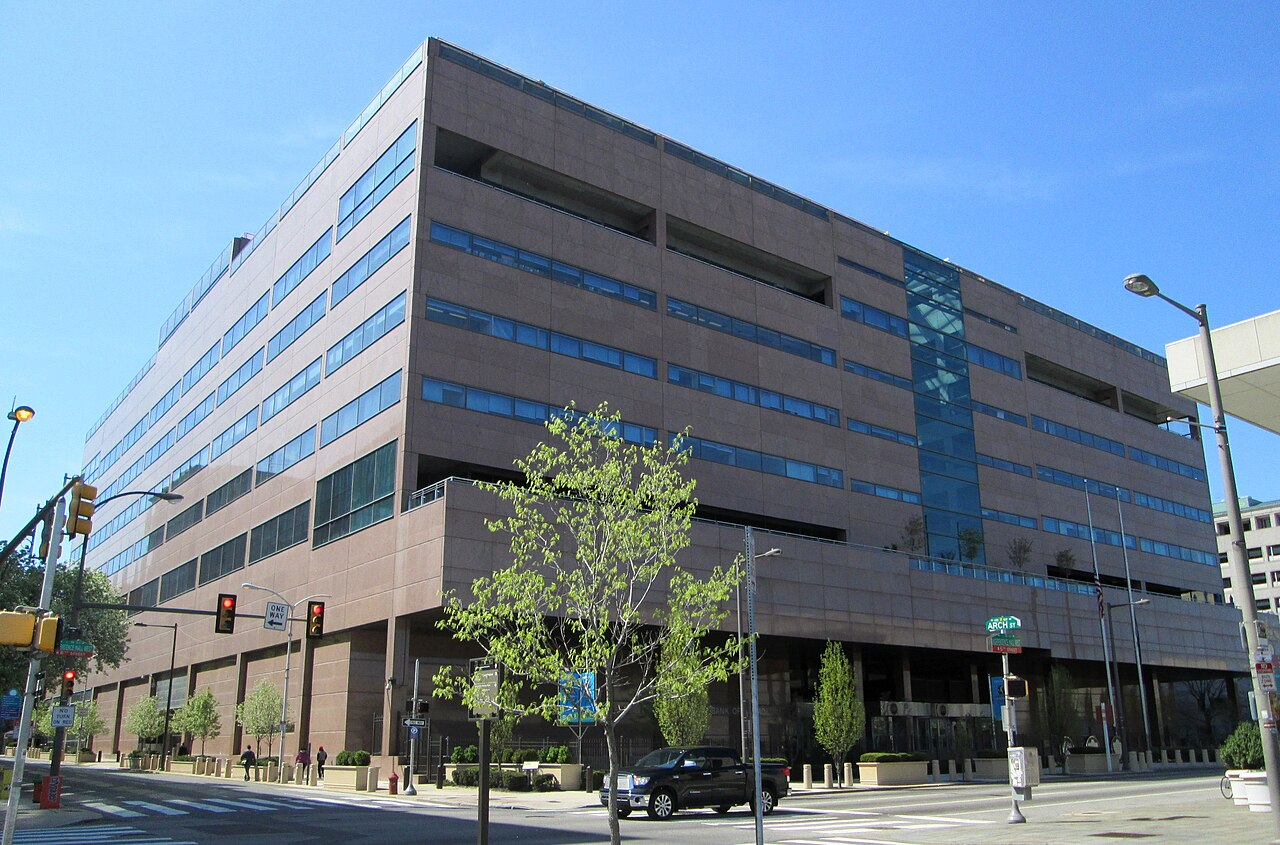
\includegraphics[height=0.30\textheight]{ch1_fed_philadelphia_2013.jpg}\\[1mm]
\imgcap{Federal Reserve Bank of Philadelphia, unde se află SPF din 1990}
\imgcredit{https://commons.wikimedia.org/wiki/File:Federal_Reserve_Bank_Building_Philadelphia.jpg}{Foto: Beyond My Ken (2013); CC BY-SA 4.0; Wikimedia Commons}
\end{column}
\begin{column}{0.66\textwidth}
\begin{itemize}
    \item \refGKMT\ compară scheme de combinare pe Survey of Professional Forecasters al BCE: ponderi egale, mediana, media trunchiată, ponderi după performanță, shrinkage și altele
    \begin{itemize}
        \item răspunsul lor: rareori și nu robust în timp
    \end{itemize}
    \item Aplicăm schemele lor pe SPF din SUA: inflația IPC (anualizată, trimestrială) la patru trimestre după trimestrul anchetei; anchete T1 1990--T2 2025 ($P = 142$, 195 de prognozatori, în medie 36 pe anchetă)
    \begin{itemize}
        \item ponderi după performanță: inversul MSE pe ultimele 20 de anchete cu realizare cunoscută, cel puțin 8 prognoze trecute (în medie 25 de prognozatori eligibili); media trunchiată: 10\% din fiecare parte
    \end{itemize}
\end{itemize}
\end{column}
\end{columns}
\end{frame}

\begin{frame}{Prognozele individuale SPF și realizarea}
\itemsize{\footnotesize}
\begin{center}
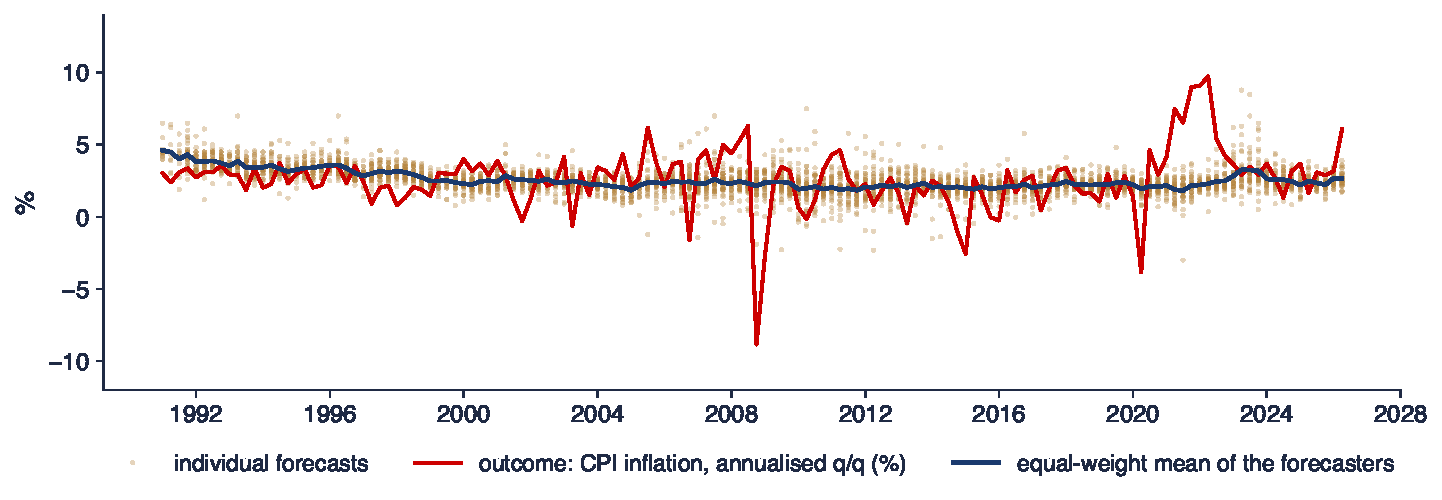
\includegraphics[width=0.97\textwidth,height=0.64\textheight,keepaspectratio]{ats_ch1_spf.pdf}
\end{center}
\vspace{-0.25cm}
\begin{itemize}
    \item Fiecare punct: prognoza IPC a unui prognozator pentru trimestrul de peste patru trimestre, plasată la trimestrul-țintă; realizarea este mult mai volatilă decît orice prognoză
\end{itemize}
\quantlet{ATS\_ch1\_spf\_combination}{\qlurl{ATS_ch1_spf_combination}}
\end{frame}

\begin{frame}{Scheme de combinare față de medie}
\itemsize{\footnotesize}
\begin{center}
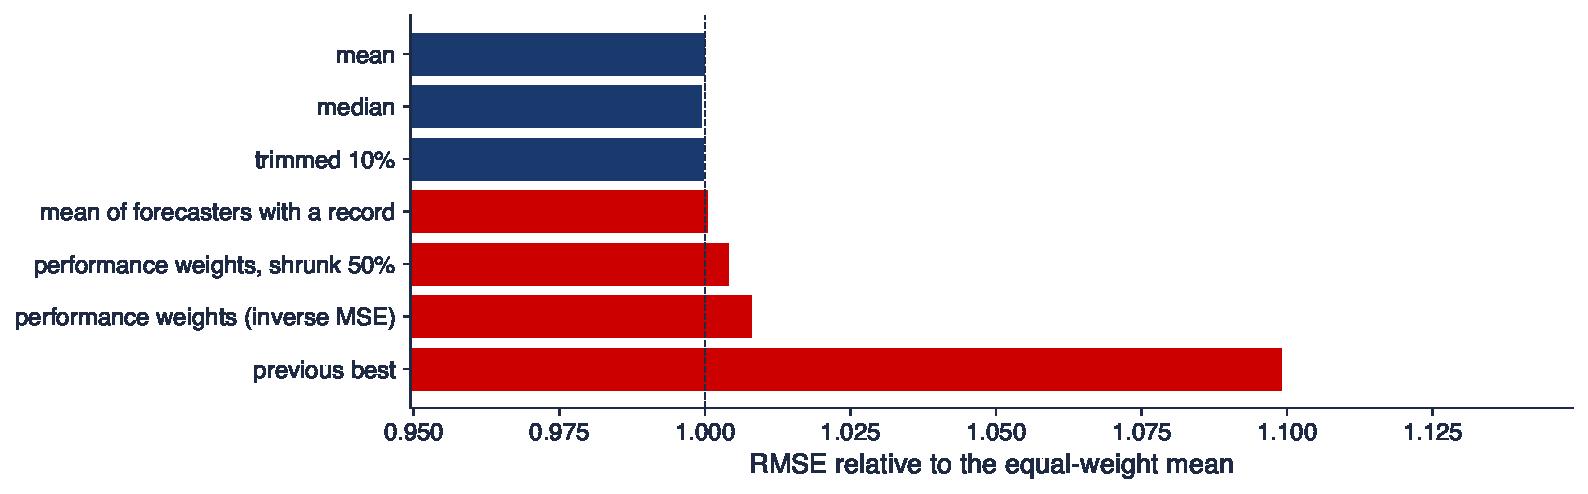
\includegraphics[width=0.97\textwidth,height=0.44\textheight,keepaspectratio]{ats_ch1_spf_schemes.pdf}
\end{center}
\vspace{-0.25cm}
\begin{itemize}
    \item RMSE relativ la media cu ponderi egale (RMSE 2{,}18 puncte procentuale); albastru: cel puțin la fel de bun ca media
\end{itemize}
\quantlet{ATS\_ch1\_spf\_combination}{\qlurl{ATS_ch1_spf_combination}}
\end{frame}

\begin{frame}{Interpretarea combinării SPF}
\itemsize{\footnotesize}
\begin{itemize}
    \item Mediana 0{,}999, media trunchiată 1{,}000, inversul MSE 1{,}008, cel mai bun anterior 1{,}099 (RMSE relativ)
    \begin{itemize}
        \item DM--HLN față de medie: mediana $p$ 0{,}842; inversul MSE $p$ 0{,}091; cel mai bun anterior HLN 2{,}76, $p$ 0{,}007
        \item Răspunsul lui \refGKMT\ se confirmă pe datele SUA: nimic nu bate media semnificativ, iar urmărirea cîștigătorului trecut pierde
    \end{itemize}
    \item Totuși 33\% dintre cei 76 de prognozatori cu cel puțin 20 de prognoze au RMSE mai mic decît media
    \begin{itemize}
        \item sînt cunoscuți doar ex post, pe eșantioane diferite și mai scurte: supraviețuire și noroc, nu abilitate care putea fi selectată
    \end{itemize}
    \item Mincer--Zarnowitz pentru medie: $\hat b = 0{,}24$ (SE 0{,}31), $R^2 = 0{,}005$, $p$ $<$\,0{,}001: inflația IPC trimestrială cu un an înainte este aproape imprevizibilă; prognozele sînt netede, realizările zgomotoase
\end{itemize}
\end{frame}

\begin{frame}{Lecțiile competițiilor M4 și M5}
\itemsize{\small}
\begin{itemize}
    \item \textbf{M4} (2018) \refMd: 100\,000 de serii, 61 de metode, prognoze punctuale și intervale de 95\%
    \begin{itemize}
        \item cîștigătorul a fost un hibrid între netezirea exponențială și o rețea neuronală recurentă; locul doi, o combinație de metode statistice cu ponderi învățate de un meta-model
        \item combinațiile au dominat primele locuri; metodele de machine learning pure au avut rezultate slabe; intervalele de predicție au fost prea înguste pentru majoritatea metodelor
    \end{itemize}
    \item \textbf{M5} (2020) \refMe: 42\,840 de serii ierarhice de vînzări Walmart, erori scalate ponderate
    \begin{itemize}
        \item arborii cu gradient boosting (LightGBM) antrenați \emph{pe toate} seriile au cîștigat; variabilele exogene (prețuri, evenimente) și învățarea între serii au contat
        \item din nou, ansamblurile de multe modele au fost în frunte (\atschlink{https://danpele.github.io/Advanced-Time-Series/RO/Cursuri/capitol12_machine_learning_deep_learning.pdf}{Capitolul 12})
    \end{itemize}
    \item Lecția comună: combinați, evaluați cu scoruri independente de scală (MASE, \atschlink{https://danpele.github.io/Time-Series-Analysis/RO/Cursuri/capitol0_introducere.pdf}{TSA, Capitolul 0}) și cu scoruri proprii și raportați o incertitudine calibrată
\end{itemize}
\end{frame}

\begin{frame}{Recapitulare: combinarea}
\itemsize{\small}
\begin{itemize}
    \item Ponderile optime reduc varianța erorii; ponderile estimate adaugă un cost de ordinul $1/n$
    \item Paradoxul: cînd prognozele sînt asemănătoare, cîștigă ponderile egale, mediana și media trunchiată
    \item Combinările liniare de densități sînt supradispersate; estimați-le prin scorul logaritmic
    \item SPF din SUA: nicio schemă nu bate media semnificativ; alegerea cîștigătorului trecut pierde
\end{itemize}
\end{frame}


%=============================================================================
\section{Date în timp real}
%=============================================================================

\begin{frame}{Versiuni ale datelor și revizuiri}
\itemsize{\small}
\begin{itemize}
    \item Datele macroeconomice se revizuiesc: PIB-ul SUA este publicat prima dată la aproximativ 30 de zile după trimestru și revizuit ani la rînd (revizuiri de referință, metode noi)
    \begin{itemize}
        \item o \textbf{versiune} este setul de date așa cum era disponibil la o anumită dată; setul de date în timp real păstrează toate versiunile \refCS
    \end{itemize}
    \item Surse fără cheie: ALFRED (St.\ Louis Fed, versiunile seriilor FRED), RTDSM al Philadelphia Fed; BCE păstrează o bază de date în timp real pentru zona euro; INS publică o estimare semnal a PIB și estimări revizuite ulterior
    \begin{itemize}
        \item prognozele făcute cu ultima versiune a datelor exagerează ce se putea prezice în timp real \refSC, \refCr
    \end{itemize}
    \item Întrebarea pentru evaluare: ce versiune este „adevărul”? Prima publicare (ținta prognozatorilor) sau ultima (cea mai bună estimare a realității)?
\end{itemize}
\end{frame}

\begin{frame}{Creșterea PIB real în SUA: prima publicare și ultima versiune}
\itemsize{\footnotesize}
\begin{center}
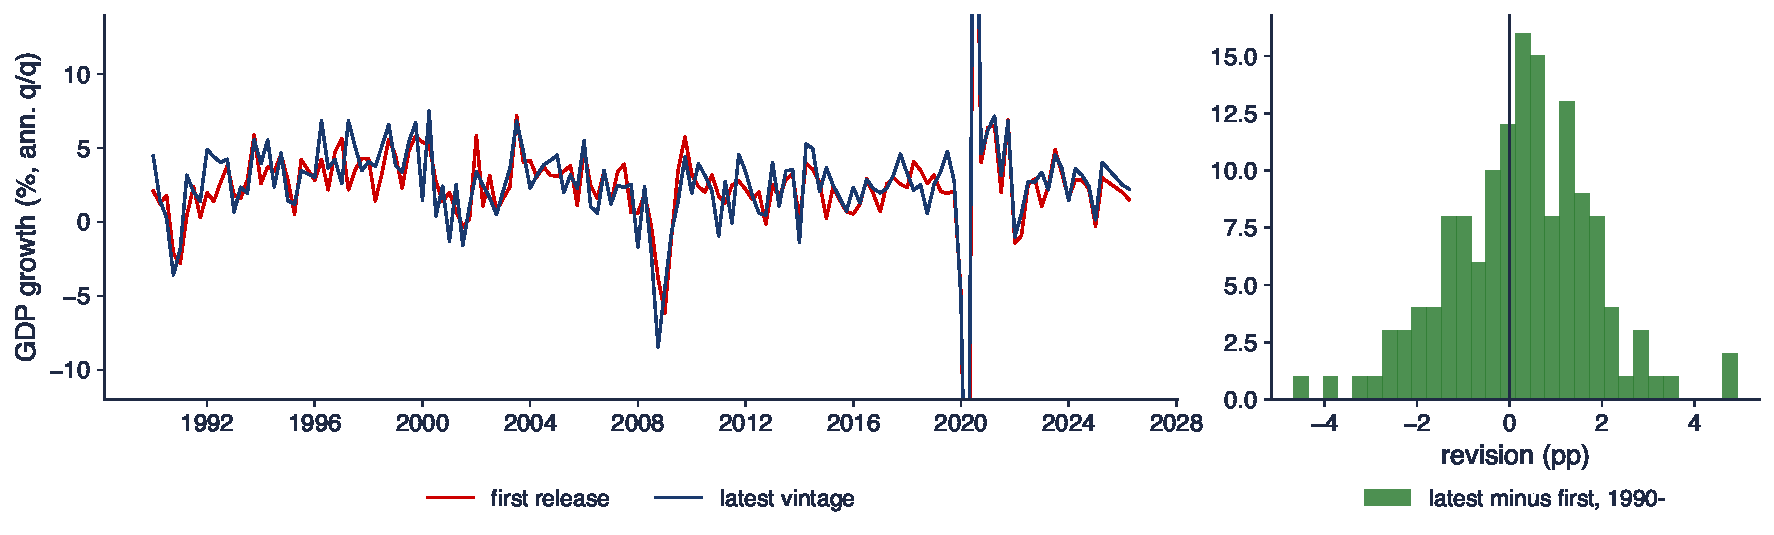
\includegraphics[width=0.97\textwidth,height=0.48\textheight,keepaspectratio]{ats_ch1_realtime.pdf}
\end{center}
\vspace{-0.25cm}
\begin{itemize}
    \item Creșterea trimestrială anualizată, 1990--2026; revizuirile = ultima versiune minus prima publicare (Philadelphia Fed RTDSM); prima publicare pentru T4 2025 lipsește (închiderea guvernului federal)
\end{itemize}
\quantlet{ATS\_ch1\_real\_time}{\qlurl{ATS_ch1_real_time}}
\end{frame}

\begin{frame}{Interpretarea revizuirilor}
\itemsize{\small}
\begin{itemize}
    \item Revizuirea medie 0{,}23 pp, abaterea standard 1{,}54 pp, revizuirea absolută medie 1{,}21 pp pe 143 de trimestre; corelația prima--ultima 0{,}939
    \begin{itemize}
        \item cele mai mari: T2 2020 (4{,}9 pp) și T4 2008 (\ensuremath{-}4{,}7 pp): revizuirile sînt mari exact la punctele de cotitură
    \end{itemize}
    \item Nowcast-ul SPF pentru trimestrul curent ($P = 143$): RMSE 1{,}95 față de prima publicare, 2{,}36 față de ultima; panta MZ 1{,}15 și 1{,}08
    \item Ierarhia prognozatorilor și a modelelor se poate schimba cu versiunea: precizați alegerea în preînregistrare
\end{itemize}
\end{frame}

\begin{frame}{Un plan de evaluare preînregistrat}
\itemsize{\small}
\begin{itemize}
    \item Fixați \textbf{înainte} de a vedea rezultatele în afara eșantionului
    \begin{itemize}
        \item ținta, orizonturile, pierderea sau scorul (secțiunile 1--3), versiunea realizării, perioada de evaluare, schema și fereastra de estimare
        \item reperul (mersul aleator, naiv sezonier, media anchetei) și lista completă a modelelor concurente
        \item testele: DM--HLN sau GW; Clark--West pentru modele imbricate; SPA sau MCS pentru multe modele; o corecție pentru mai multe orizonturi (Holm)
    \end{itemize}
    \item Raportați tot ce s-a încercat; un model selectat pe perioada de test are o eroare deplasată
    \begin{itemize}
        \item proiectul acestui curs începe exact cu un astfel de plan (propunerea și preînregistrarea, 5\%)
    \end{itemize}
\end{itemize}
\end{frame}

\begin{frame}{Recapitulare: date în timp real}
\itemsize{\small}
\begin{itemize}
    \item Evaluați prognozele cu datele care existau cînd au fost făcute
    \item Revizuirile sînt mari la punctele de cotitură; alegerea versiunii „adevărate” schimbă RMSE și ierarhiile
    \item Preînregistrați țintele, pierderile, reperele, testele și versiunea datelor
\end{itemize}
\end{frame}


%=============================================================================
\section{AI în descoperirea științifică}
%=============================================================================

\begin{frame}{O întrebare deschisă}
\itemsize{\small}
\begin{itemize}
    \item Rezistă paradoxul combinării cînd panelul de experți se schimbă în timp, iar distribuția realizărilor se deplasează (2020--2023)?
    \begin{itemize}
        \item formal: $H_0$: $\E[(y - \hat y_{\lambda})^2 - (y - \bar y)^2] \ge 0$ pentru orice factor de shrinkage $\lambda$ fixat dinainte, în fiecare subperioadă
        \item $\hat y_\lambda$: combinația shrinkage cu factorul $\lambda$; $\bar y$: media tuturor prognozatorilor
        \item infirmată de un $\lambda$ preînregistrat care bate media cu DM--HLN și p-value $< 0{,}05$ după o corecție Holm pe subperioade
    \end{itemize}
    \item De ce contează: băncile centrale publică media anchetelor; o combinare mai bună ar schimba așteptările publicate
    \begin{itemize}
        \item literatura de pornire: \refGKMT, \refCT, \refSWal, \refCMVW, \refWHLK
    \end{itemize}
\end{itemize}
\end{frame}

\begin{frame}{Bucla de cercetare cu un asistent AI}
\itemsize{\footnotesize}
\begin{itemize}
    \item Un asistent AI (un LLM precum Claude, ChatGPT, Gemini sau Copilot) accelerează fiecare etapă; Semantic Scholar și Elicit ajută la literatură
    \begin{itemize}
        \item \textbf{literatura}: \aiprompt{Listează articole recenzate despre combinarea prognozelor SPF cu intrarea și ieșirea prognozatorilor; dă DOI-urile.} Apoi verificați fiecare DOI pe Crossref
        \item \textbf{ipoteza}: \aiprompt{Propune trei motive pentru care ponderile după inversul MSE ar putea bate media după 2020, fiecare cu un test.}
        \item \textbf{cod și replicare}: cereți o funcție, apoi reproduceți întîi o cifră cunoscută (RMSE relativ al medianei din acest curs)
        \item \textbf{robustețe și critică}: \aiprompt{Joacă rolul unui recenzent ostil: enumeră toate felurile în care această evaluare ar putea fi afectată de data snooping.}
    \end{itemize}
    \item Raportul: ce s-a cerut, ce s-a păstrat, ce s-a respins (AI\_USE.md, AI\_ERRORS.md)
\end{itemize}
\end{frame}

\begin{frame}{Verificări necesare}
\itemsize{\small}
\begin{itemize}
    \item Fiecare referință există și spune ce se afirmă (DOI-ul funcționează, titlul coincide, rezultatul se află în lucrare)
    \item Fără informație din viitor: ponderile la ancheta $s$ folosesc doar realizări cunoscute la $s$ (aici, prognoze din anchete cu cel puțin cinci trimestre mai vechi, al căror trimestru-țintă s-a încheiat)
    \item Numărul de laguri HAC corespunde suprapunerii țintelor ($h - 1$); corecția HLN este aplicată
    \item $\lambda$, subperioadele și istoricul minim sînt fixate înaintea rezultatelor; toate variantele sînt raportate
    \item Interpretarea separă „nesemnificativ” de „egal”
\end{itemize}
\end{frame}

\begin{frame}{Mini-studiu de caz: shrinkage pe subperioade}
\itemsize{\footnotesize}
\begin{center}
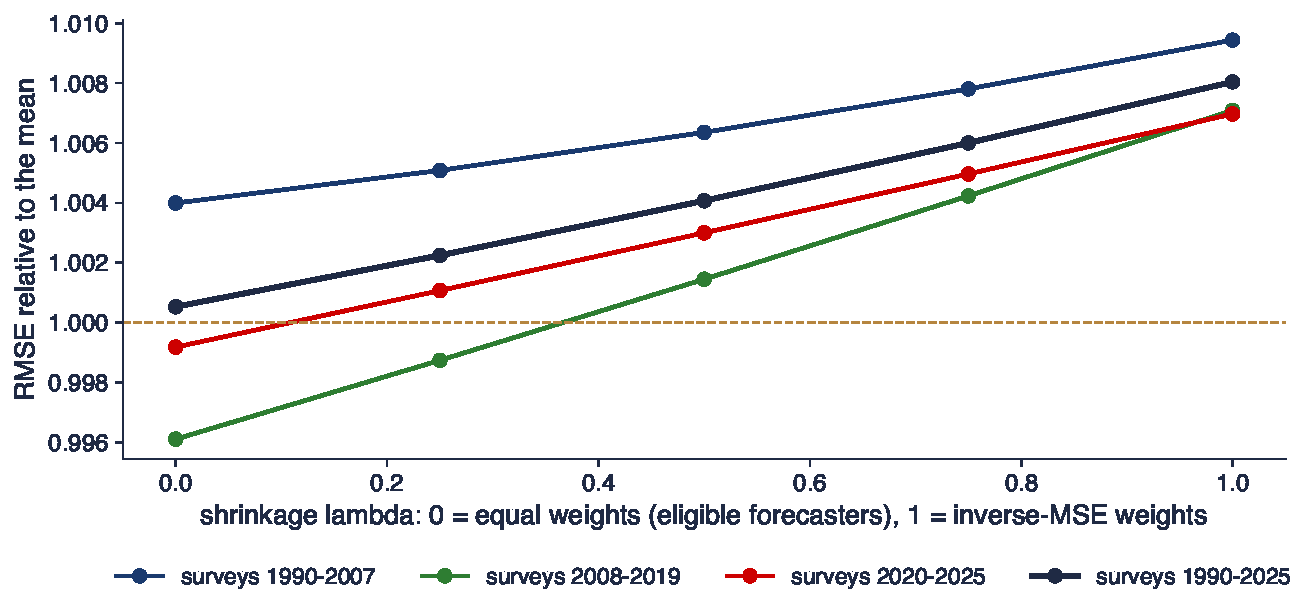
\includegraphics[width=0.97\textwidth,height=0.46\textheight,keepaspectratio]{ats_ch1_ai_case.pdf}
\end{center}
\vspace{-0.25cm}
\begin{itemize}
    \item RMSE al combinației $\lambda\cdot$(ponderi după inversul MSE) + $(1 - \lambda)\cdot$(ponderi egale între prognozatorii eligibili), relativ la media tuturor prognozatorilor; SPF din SUA, IPC la patru trimestre
    \item $\lambda = 1$: 1{,}009 (1990--2007, $P = 72$), 1{,}007 (2008--2019), 1{,}007 (2020--2025); eșantionul complet HLN 1{,}70, $p$ 0{,}091
    \item În fiecare subperioadă: cu cît ponderea performanței trecute este mai mare, cu atît rezultatul este mai slab; paradoxul rezistă valului inflaționist din 2020--2023
\end{itemize}
\quantlet{ATS\_ch1\_spf\_combination}{\qlurl{ATS_ch1_spf_combination}}
\end{frame}

\begin{frame}{Idee de proiect}
\itemsize{\small}
\begin{itemize}
    \item \textbf{Combinarea prognozelor inflației din România}: modele (AR, curba Phillips cu deviația PIB, ținta BNR), anchete și așteptări din piață
    \begin{itemize}
        \item preînregistrați orizonturile de 1--12 luni, pierderea pinball la 5\%, 50\%, 95\% și CRPS, corecția Holm pe orizonturi
        \item replicați întîi: tabelul pentru inflația din România din acest curs (Seminarul 1, C1 îl face pe orizonturi)
        \item extensie: combinarea densităților prin optimal pools; testul GW pentru a vedea dacă șocul din 2022 a schimbat cîștigătorul
    \end{itemize}
    \item Livrabilele urmează regulile cursului: repository, raport, AI\_USE.md, AI\_ERRORS.md, susținere orală
\end{itemize}
\end{frame}


%=============================================================================
\section{Încheiere}
%=============================================================================

\begin{frame}{Idei de reținut}
\itemsize{\small}
\begin{itemize}
    \item Alegeți întîi pierderea sau scorul: ele definesc ce este o prognoză „bună” (medie, mediană, cuantilă, distribuție)
    \item Prognozele de densitate: verificați calibrarea cu PIT, ierarhizați cu scoruri proprii; ES are nevoie de VaR pentru a fi evaluat
    \item Teste: DM--HLN cu HAC, GW pentru metode, Clark--West pentru modele imbricate, SPA și MCS pentru multe modele
    \item Combinați prognozele asemănătoare cu ponderi egale; ponderile estimate merită doar pentru prognoze foarte diferite și istoric lung
    \item Evaluați în timp real și preînregistrați planul
\end{itemize}
\end{frame}

\begin{frame}{Autoevaluare}
\itemsize{\small}
\begin{columns}[T]
\begin{column}{0.56\textwidth}
\begin{block}{Întrebări}
\begin{itemize}
    \item Ce funcțională elicitează pierderea pinball cu $\tau = 0{,}05$?
    \item Ce spune o histogramă PIT în formă de U despre intervale?
    \item De ce nu este valid testul DM pentru modele imbricate cu parametri estimați?
    \item Cînd bat ponderile de combinare estimate ponderile egale?
    \item De ce nu poate fi ierarhizat ES singur?
\end{itemize}
\end{block}
\end{column}
\begin{column}{0.40\textwidth}
\begin{block}{Urmează: \atschlink{https://danpele.github.io/Advanced-Time-Series/RO/Cursuri/capitol2_rupturi_structurale_modele_neliniare.pdf}{Capitolul 2}}
\begin{itemize}
    \item Rupturi structurale și modele neliniare: teste pentru rupturi, modele cu prag
    \item Evaluarea prognozelor sub instabilitate: ferestre mobile, eșecul prognozelor, testul de fluctuație \refGRaz
\end{itemize}
\end{block}
\end{column}
\end{columns}
\end{frame}


%=============================================================================
\section{Anexă}
%=============================================================================

\begin{frame}{Anexă: consistența pierderii pinball}
\hypertarget{atsapp1}{}\atsappback{atssrc1}{Înapoi}
\itemsize{\small}
\begin{itemize}
    \item $\E\rho_\tau(Y - x) = \tau\int_x^\infty(y - x)dF(y) + (1 - \tau)\int_{-\infty}^x(x - y)dF(y)$
    \item Derivata (Leibniz): $-\tau(1 - F(x)) + (1 - \tau)F(x) = F(x) - \tau$; nulă în $x = F^{-1}(\tau)$; derivata a doua $f(x) \ge 0$
    \item Pentru $\tau = 1/2$: $\rho_{1/2}(e) = |e|/2$, deci mediana; pentru $x$ diferit de cuantilă, pierderea suplimentară este $\int_q^x(F(z) - \tau)dz > 0$
    \item Pierderile liniare pe porțiuni generalizate $(\mathbf 1\{y \le x\} - \tau)(g(x) - g(y))$, $g$ crescătoare, formează întreaga clasă de pierderi consistente pentru cuantilă \refGnaa
\end{itemize}
\end{frame}

\begin{frame}{Anexă: forma cu nucleu a CRPS}
\hypertarget{atsapp2}{}\atsappback{atssrc2}{Înapoi}
\itemsize{\small}
\begin{itemize}
    \item Scriem $(F(z) - \mathbf 1\{y \le z\})^2 = F(z)^2 - 2F(z)\mathbf 1\{y \le z\} + \mathbf 1\{y \le z\}$
    \item Cu $X, X' \sim F$ i.i.d.: $F(z)^2 = P(X \le z, X' \le z)$ și $\E|X - y| = \int[F(z)(1 - \mathbf 1\{y \le z\}) + (1 - F(z))\mathbf 1\{y \le z\}]dz$
    \item $\frac12\E|X - X'| = \int F(z)(1 - F(z))dz$; prin scădere obținem $\int(F(z) - \mathbf 1\{y \le z\})^2dz$
    \item Proprietatea: $\E_G\mathrm{CRPS}(F, Y) - \E_G\mathrm{CRPS}(G, Y) = \int(F(z) - G(z))^2dz \ge 0$, zero doar dacă $F = G$
\end{itemize}
\end{frame}

\begin{frame}{Anexă: corecția Clark--West}
\hypertarget{atsapp3}{}\atsappback{atssrc3}{Înapoi}
\itemsize{\small}
\begin{itemize}
    \item Sub $H_0$ coeficienții suplimentari ai modelului mare sînt $\beta_2 = 0$; prognoza lui este aproximativ $\hat y_2 = \hat y_1 + \hat\beta_2'x_{2}$, cu $\hat\beta_2$ zgomot de estimare pur
    \item $e_2 = e_1 - (\hat y_2 - \hat y_1)$, deci $e_1^2 - e_2^2 = 2e_1(\hat y_2 - \hat y_1) - (\hat y_2 - \hat y_1)^2$
    \item $\E[e_1(\hat y_2 - \hat y_1)] = 0$ sub $H_0$ ($e_1$ este o diferență de martingală), deci $\E(e_1^2 - e_2^2) = -\E(\hat y_2 - \hat y_1)^2 < 0$
    \item Adunarea lui $(\hat y_1 - \hat y_2)^2$ recentrează diferențialul în zero: $f_t = 2e_{1t}(\hat y_{2t} - \hat y_{1t})$, statistica de încadrare din \refHLNih\ sub altă formă
\end{itemize}
\end{frame}


%=============================================================================
\section{Bibliografie}
%=============================================================================

\begin{frame}{Bibliografie (1/7)}
\itemsize{\tiny}
\begin{itemize}
    \item Amisano, G., \& Giacomini, R. (2007). Comparing density forecasts via weighted likelihood ratio tests. \textit{Journal of Business \& Economic Statistics}, 25(2), 177--190. \href{https://doi.org/10.1198/073500106000000332}{doi:10.1198/073500106000000332}
    \item Atkeson, A., \& Ohanian, L. E. (2001). Are Phillips curves useful for forecasting inflation? \textit{Federal Reserve Bank of Minneapolis Quarterly Review}, 25(1), 2--11. \href{https://doi.org/10.21034/qr.2511}{doi:10.21034/qr.2511}
    \item Banerjee, A., Guo, X., \& Wang, H. (2005). On the optimality of conditional expectation as a Bregman predictor. \textit{IEEE Transactions on Information Theory}, 51(7), 2664--2669. \href{https://doi.org/10.1109/TIT.2005.850145}{doi:10.1109/TIT.2005.850145}
    \item Bates, J. M., \& Granger, C. W. J. (1969). The combination of forecasts. \textit{Operational Research Quarterly}, 20(4), 451--468. \href{https://doi.org/10.1057/jors.1969.103}{doi:10.1057/jors.1969.103}
    \item Berkowitz, J. (2001). Testing density forecasts, with applications to risk management. \textit{Journal of Business \& Economic Statistics}, 19(4), 465--474. \href{https://doi.org/10.1198/07350010152596718}{doi:10.1198/07350010152596718}
    \item Bollerslev, T. (1987). A conditionally heteroskedastic time series model for speculative prices and rates of return. \textit{The Review of Economics and Statistics}, 69(3), 542--547. \href{https://doi.org/10.2307/1925546}{doi:10.2307/1925546}
    \item Brier, G. W. (1950). Verification of forecasts expressed in terms of probability. \textit{Monthly Weather Review}, 78(1), 1--3. \href{https://doi.org/10.1175/1520-0493(1950)078\%3C0001:VOFEIT\%3E2.0.CO;2}{doi:10.1175/1520-0493(1950)078\textless{}0001:VOFEIT\textgreater{}2.0.CO;2}
    \item Capistrán, C., \& Timmermann, A. (2009). Forecast combination with entry and exit of experts. \textit{Journal of Business \& Economic Statistics}, 27(4), 428--440. \href{https://doi.org/10.1198/jbes.2009.07211}{doi:10.1198/jbes.2009.07211}
    \item Chong, Y. Y., \& Hendry, D. F. (1986). Econometric evaluation of linear macro-economic models. \textit{The Review of Economic Studies}, 53(4), 671--690. \href{https://doi.org/10.2307/2297611}{doi:10.2307/2297611}
    \item Christoffersen, P. F., \& Diebold, F. X. (1997). Optimal prediction under asymmetric loss. \textit{Econometric Theory}, 13(6), 808--817. \href{https://doi.org/10.1017/S0266466600006277}{doi:10.1017/S0266466600006277}
    \item Christoffersen, P. F. (1998). Evaluating interval forecasts. \textit{International Economic Review}, 39(4), 841--862. \href{https://doi.org/10.2307/2527341}{doi:10.2307/2527341}
    \item Claeskens, G., Magnus, J. R., Vasnev, A. L., \& Wang, W. (2016). The forecast combination puzzle: A simple theoretical explanation. \textit{International Journal of Forecasting}, 32(3), 754--762. \href{https://doi.org/10.1016/j.ijforecast.2015.12.005}{doi:10.1016/j.ijforecast.2015.12.005}
\end{itemize}
\end{frame}

\begin{frame}{Bibliografie (2/7)}
\itemsize{\tiny}
\begin{itemize}
    \item Clark, T. E., \& McCracken, M. W. (2001). Tests of equal forecast accuracy and encompassing for nested models. \textit{Journal of Econometrics}, 105(1), 85--110. \href{https://doi.org/10.1016/S0304-4076(01)00071-9}{doi:10.1016/S0304-4076(01)00071-9}
    \item Clark, T. E., \& West, K. D. (2007). Approximately normal tests for equal predictive accuracy in nested models. \textit{Journal of Econometrics}, 138(1), 291--311. \href{https://doi.org/10.1016/j.jeconom.2006.05.023}{doi:10.1016/j.jeconom.2006.05.023}
    \item Croushore, D. (2011). Frontiers of real-time data analysis. \textit{Journal of Economic Literature}, 49(1), 72--100. \href{https://doi.org/10.1257/jel.49.1.72}{doi:10.1257/jel.49.1.72}
    \item Croushore, D., \& Stark, T. (2001). A real-time data set for macroeconomists. \textit{Journal of Econometrics}, 105(1), 111--130. \href{https://doi.org/10.1016/S0304-4076(01)00072-0}{doi:10.1016/S0304-4076(01)00072-0}
    \item Dawid, A. P. (1984). Statistical theory: The prequential approach. \textit{Journal of the Royal Statistical Society, Series A}, 147(2), 278--292. \href{https://doi.org/10.2307/2981683}{doi:10.2307/2981683}
    \item Diebold, F. X. (2015). Comparing predictive accuracy, twenty years later: A personal perspective on the use and abuse of Diebold--Mariano tests. \textit{Journal of Business \& Economic Statistics}, 33(1), 1. \href{https://doi.org/10.1080/07350015.2014.983236}{doi:10.1080/07350015.2014.983236}
    \item Diebold, F. X., Gunther, T. A., \& Tay, A. S. (1998). Evaluating density forecasts with applications to financial risk management. \textit{International Economic Review}, 39(4), 863--883. \href{https://doi.org/10.2307/2527342}{doi:10.2307/2527342}
    \item Diebold, F. X., \& Mariano, R. S. (1995). Comparing predictive accuracy. \textit{Journal of Business \& Economic Statistics}, 13(3), 253--263. \href{https://doi.org/10.1080/07350015.1995.10524599}{doi:10.1080/07350015.1995.10524599}
    \item Diebold, F. X., \& Pauly, P. (1990). The use of prior information in forecast combination. \textit{International Journal of Forecasting}, 6(4), 503--508. \href{https://doi.org/10.1016/0169-2070(90)90028-A}{doi:10.1016/0169-2070(90)90028-A}
    \item Ehm, W., Gneiting, T., Jordan, A., \& Krüger, F. (2016). Of quantiles and expectiles: Consistent scoring functions, Choquet representations and forecast rankings. \textit{Journal of the Royal Statistical Society, Series B}, 78(3), 505--562. \href{https://doi.org/10.1111/rssb.12154}{doi:10.1111/rssb.12154}
    \item Elliott, G., \& Timmermann, A. (2008). Economic forecasting. \textit{Journal of Economic Literature}, 46(1), 3--56. \href{https://doi.org/10.1257/jel.46.1.3}{doi:10.1257/jel.46.1.3}
    \item Fama, E. F. (1984). Forward and spot exchange rates. \textit{Journal of Monetary Economics}, 14(3), 319--338. \href{https://doi.org/10.1016/0304-3932(84)90046-1}{doi:10.1016/0304-3932(84)90046-1}
\end{itemize}
\end{frame}

\begin{frame}{Bibliografie (3/7)}
\itemsize{\tiny}
\begin{itemize}
    \item Fissler, T., \& Ziegel, J. F. (2016). Higher order elicitability and Osband's principle. \textit{The Annals of Statistics}, 44(4), 1680--1707. \href{https://doi.org/10.1214/16-AOS1439}{doi:10.1214/16-AOS1439}
    \item Genre, V., Kenny, G., Meyler, A., \& Timmermann, A. (2013). Combining expert forecasts: Can anything beat the simple average? \textit{International Journal of Forecasting}, 29(1), 108--121. \href{https://doi.org/10.1016/j.ijforecast.2012.06.004}{doi:10.1016/j.ijforecast.2012.06.004}
    \item Geweke, J., \& Amisano, G. (2011). Optimal prediction pools. \textit{Journal of Econometrics}, 164(1), 130--141. \href{https://doi.org/10.1016/j.jeconom.2011.02.017}{doi:10.1016/j.jeconom.2011.02.017}
    \item Giacomini, R., \& Rossi, B. (2010). Forecast comparisons in unstable environments. \textit{Journal of Applied Econometrics}, 25(4), 595--620. \href{https://doi.org/10.1002/jae.1177}{doi:10.1002/jae.1177}
    \item Giacomini, R., \& White, H. (2006). Tests of conditional predictive ability. \textit{Econometrica}, 74(6), 1545--1578. \href{https://doi.org/10.1111/j.1468-0262.2006.00718.x}{doi:10.1111/j.1468-0262.2006.00718.x}
    \item Gneiting, T., Balabdaoui, F., \& Raftery, A. E. (2007). Probabilistic forecasts, calibration and sharpness. \textit{Journal of the Royal Statistical Society, Series B}, 69(2), 243--268. \href{https://doi.org/10.1111/j.1467-9868.2007.00587.x}{doi:10.1111/j.1467-9868.2007.00587.x}
    \item Gneiting, T., \& Katzfuss, M. (2014). Probabilistic forecasting. \textit{Annual Review of Statistics and Its Application}, 1, 125--151. \href{https://doi.org/10.1146/annurev-statistics-062713-085831}{doi:10.1146/annurev-statistics-062713-085831}
    \item Gneiting, T. (2011). Making and evaluating point forecasts. \textit{Journal of the American Statistical Association}, 106(494), 746--762. \href{https://doi.org/10.1198/jasa.2011.r10138}{doi:10.1198/jasa.2011.r10138}
    \item Gneiting, T., \& Raftery, A. E. (2007). Strictly proper scoring rules, prediction, and estimation. \textit{Journal of the American Statistical Association}, 102(477), 359--378. \href{https://doi.org/10.1198/016214506000001437}{doi:10.1198/016214506000001437}
    \item Gneiting, T., \& Ranjan, R. (2013). Combining predictive distributions. \textit{Electronic Journal of Statistics}, 7, 1747--1782. \href{https://doi.org/10.1214/13-EJS823}{doi:10.1214/13-EJS823}
    \item Gneiting, T., \& Ranjan, R. (2011). Comparing density forecasts using threshold- and quantile-weighted scoring rules. \textit{Journal of Business \& Economic Statistics}, 29(3), 411--422. \href{https://doi.org/10.1198/jbes.2010.08110}{doi:10.1198/jbes.2010.08110}
    \item Good, I. J. (1952). Rational decisions. \textit{Journal of the Royal Statistical Society, Series B}, 14(1), 107--114. \href{https://doi.org/10.1111/j.2517-6161.1952.tb00104.x}{doi:10.1111/j.2517-6161.1952.tb00104.x}
\end{itemize}
\end{frame}

\begin{frame}{Bibliografie (4/7)}
\itemsize{\tiny}
\begin{itemize}
    \item Granger, C. W. J., \& Ramanathan, R. (1984). Improved methods of combining forecasts. \textit{Journal of Forecasting}, 3(2), 197--204. \href{https://doi.org/10.1002/for.3980030207}{doi:10.1002/for.3980030207}
    \item Hall, S. G., \& Mitchell, J. (2007). Combining density forecasts. \textit{International Journal of Forecasting}, 23(1), 1--13. \href{https://doi.org/10.1016/j.ijforecast.2006.08.001}{doi:10.1016/j.ijforecast.2006.08.001}
    \item Hamill, T. M. (2001). Interpretation of rank histograms for verifying ensemble forecasts. \textit{Monthly Weather Review}, 129(3), 550--560. \href{https://doi.org/10.1175/1520-0493(2001)129\%3C0550:IORHFV\%3E2.0.CO;2}{doi:10.1175/1520-0493(2001)129\textless{}0550:IORHFV\textgreater{}2.0.CO;2}
    \item Hamilton, J. D. (1994). \textit{Time Series Analysis}. Princeton University Press. \href{https://doi.org/10.2307/j.ctv14jx6sm}{doi:10.2307/j.ctv14jx6sm}
    \item Hansen, P. R. (2005). A test for superior predictive ability. \textit{Journal of Business \& Economic Statistics}, 23(4), 365--380. \href{https://doi.org/10.1198/073500105000000063}{doi:10.1198/073500105000000063}
    \item Hansen, P. R., Lunde, A., \& Nason, J. M. (2011). The model confidence set. \textit{Econometrica}, 79(2), 453--497. \href{https://doi.org/10.3982/ECTA5771}{doi:10.3982/ECTA5771}
    \item Harvey, D. I., Leybourne, S. J., \& Newbold, P. (1998). Tests for forecast encompassing. \textit{Journal of Business \& Economic Statistics}, 16(2), 254--259. \href{https://doi.org/10.1080/07350015.1998.10524759}{doi:10.1080/07350015.1998.10524759}
    \item Harvey, D., Leybourne, S., \& Newbold, P. (1997). Testing the equality of prediction mean squared errors. \textit{International Journal of Forecasting}, 13(2), 281--291. \href{https://doi.org/10.1016/S0169-2070(96)00719-4}{doi:10.1016/S0169-2070(96)00719-4}
    \item Hong, T., \& Fan, S. (2016). Probabilistic electric load forecasting: A tutorial review. \textit{International Journal of Forecasting}, 32(3), 914--938. \href{https://doi.org/10.1016/j.ijforecast.2015.11.011}{doi:10.1016/j.ijforecast.2015.11.011}
    \item Hong, T., Pinson, P., Fan, S., Zareipour, H., Troccoli, A., \& Hyndman, R. J. (2016). Probabilistic energy forecasting: Global Energy Forecasting Competition 2014 and beyond. \textit{International Journal of Forecasting}, 32(3), 896--913. \href{https://doi.org/10.1016/j.ijforecast.2016.02.001}{doi:10.1016/j.ijforecast.2016.02.001}
    \item Huang, C., \& Petukhina, A. (2022). \textit{Applied Time Series Analysis and Forecasting with Python}. Springer. \href{https://doi.org/10.1007/978-3-031-13584-2}{doi:10.1007/978-3-031-13584-2}
    \item Hyndman, R. J., \& Koehler, A. B. (2006). Another look at measures of forecast accuracy. \textit{International Journal of Forecasting}, 22(4), 679--688. \href{https://doi.org/10.1016/j.ijforecast.2006.03.001}{doi:10.1016/j.ijforecast.2006.03.001}
\end{itemize}
\end{frame}

\begin{frame}{Bibliografie (5/7)}
\itemsize{\tiny}
\begin{itemize}
    \item Kilian, L., \& Lütkepohl, H. (2017). \textit{Structural Vector Autoregressive Analysis}. Cambridge University Press. \href{https://doi.org/10.1017/9781108164818}{doi:10.1017/9781108164818}
    \item Makridakis, S., Spiliotis, E., \& Assimakopoulos, V. (2022). M5 accuracy competition: Results, findings, and conclusions. \textit{International Journal of Forecasting}, 38(4), 1346--1364. \href{https://doi.org/10.1016/j.ijforecast.2021.11.013}{doi:10.1016/j.ijforecast.2021.11.013}
    \item Makridakis, S., Spiliotis, E., \& Assimakopoulos, V. (2020). The M4 Competition: 100,000 time series and 61 forecasting methods. \textit{International Journal of Forecasting}, 36(1), 54--74. \href{https://doi.org/10.1016/j.ijforecast.2019.04.014}{doi:10.1016/j.ijforecast.2019.04.014}
    \item Matheson, J. E., \& Winkler, R. L. (1976). Scoring rules for continuous probability distributions. \textit{Management Science}, 22(10), 1087--1096. \href{https://doi.org/10.1287/mnsc.22.10.1087}{doi:10.1287/mnsc.22.10.1087}
    \item Meese, R. A., \& Rogoff, K. (1983). Empirical exchange rate models of the seventies. \textit{Journal of International Economics}, 14(1--2), 3--24. \href{https://doi.org/10.1016/0022-1996(83)90017-X}{doi:10.1016/0022-1996(83)90017-X}
    \item Mincer, J., \& Zarnowitz, V. (1969). The evaluation of economic forecasts. In J. Mincer (Ed.), \textit{Economic Forecasts and Expectations} (pp.\ 3--46). NBER. \href{https://www.nber.org/books-and-chapters/economic-forecasts-and-expectations-analysis-forecasting-behavior-and-performance/evaluation-economic-forecasts}{nber.org}
    \item Newey, W. K., \& West, K. D. (1987). A simple, positive semi-definite, heteroskedasticity and autocorrelation consistent covariance matrix. \textit{Econometrica}, 55(3), 703--708. \href{https://doi.org/10.2307/1913610}{doi:10.2307/1913610}
    \item Patton, A. J. (2020). Comparing possibly misspecified forecasts. \textit{Journal of Business \& Economic Statistics}, 38(4), 796--809. \href{https://doi.org/10.1080/07350015.2019.1585256}{doi:10.1080/07350015.2019.1585256}
    \item Patton, A. J. (2011). Volatility forecast comparison using imperfect volatility proxies. \textit{Journal of Econometrics}, 160(1), 246--256. \href{https://doi.org/10.1016/j.jeconom.2010.03.034}{doi:10.1016/j.jeconom.2010.03.034}
    \item Petropoulos, F., Apiletti, D., Assimakopoulos, V., et al.\ (2022). Forecasting: theory and practice. \textit{International Journal of Forecasting}, 38(3), 705--871. \href{https://doi.org/10.1016/j.ijforecast.2021.11.001}{doi:10.1016/j.ijforecast.2021.11.001}
    \item Romano, J. P., \& Wolf, M. (2005). Stepwise multiple testing as formalized data snooping. \textit{Econometrica}, 73(4), 1237--1282. \href{https://doi.org/10.1111/j.1468-0262.2005.00615.x}{doi:10.1111/j.1468-0262.2005.00615.x}
    \item Rossi, B., \& Sekhposyan, T. (2019). Alternative tests for correct specification of conditional predictive densities. \textit{Journal of Econometrics}, 208(2), 638--657. \href{https://doi.org/10.1016/j.jeconom.2018.07.008}{doi:10.1016/j.jeconom.2018.07.008}
\end{itemize}
\end{frame}

\begin{frame}{Bibliografie (6/7)}
\itemsize{\tiny}
\begin{itemize}
    \item Savage, L. J. (1971). Elicitation of personal probabilities and expectations. \textit{Journal of the American Statistical Association}, 66(336), 783--801. \href{https://doi.org/10.1080/01621459.1971.10482346}{doi:10.1080/01621459.1971.10482346}
    \item Scheuerer, M., \& Hamill, T. M. (2015). Variogram-based proper scoring rules for probabilistic forecasts of multivariate quantities. \textit{Monthly Weather Review}, 143(4), 1321--1334. \href{https://doi.org/10.1175/MWR-D-14-00269.1}{doi:10.1175/MWR-D-14-00269.1}
    \item Smith, J., \& Wallis, K. F. (2009). A simple explanation of the forecast combination puzzle. \textit{Oxford Bulletin of Economics and Statistics}, 71(3), 331--355. \href{https://doi.org/10.1111/j.1468-0084.2008.00541.x}{doi:10.1111/j.1468-0084.2008.00541.x}
    \item Stark, T., \& Croushore, D. (2002). Forecasting with a real-time data set for macroeconomists. \textit{Journal of Macroeconomics}, 24(4), 507--531. \href{https://doi.org/10.1016/S0164-0704(02)00062-9}{doi:10.1016/S0164-0704(02)00062-9}
    \item Stock, J. H., \& Watson, M. W. (2004). Combination forecasts of output growth in a seven-country data set. \textit{Journal of Forecasting}, 23(6), 405--430. \href{https://doi.org/10.1002/for.928}{doi:10.1002/for.928}
    \item Stock, J. H., \& Watson, M. W. (1999). Forecasting inflation. \textit{Journal of Monetary Economics}, 44(2), 293--335. \href{https://doi.org/10.1016/S0304-3932(99)00027-6}{doi:10.1016/S0304-3932(99)00027-6}
    \item Timmermann, A. (2006). Forecast combinations. In G. Elliott, C. W. J. Granger, \& A. Timmermann (Eds.), \textit{Handbook of Economic Forecasting} (Vol.\ 1, pp.\ 135--196). Elsevier. \href{https://doi.org/10.1016/S1574-0706(05)01004-9}{doi:10.1016/S1574-0706(05)01004-9}
    \item Wang, X., Hyndman, R. J., Li, F., \& Kang, Y. (2023). Forecast combinations: An over 50-year review. \textit{International Journal of Forecasting}, 39(4), 1518--1547. \href{https://doi.org/10.1016/j.ijforecast.2022.11.005}{doi:10.1016/j.ijforecast.2022.11.005}
    \item Weber, S. (2006). Distribution-invariant risk measures, information, and dynamic consistency. \textit{Mathematical Finance}, 16(2), 419--441. \href{https://doi.org/10.1111/j.1467-9965.2006.00277.x}{doi:10.1111/j.1467-9965.2006.00277.x}
    \item Welch, I., \& Goyal, A. (2008). A comprehensive look at the empirical performance of equity premium prediction. \textit{The Review of Financial Studies}, 21(4), 1455--1508. \href{https://doi.org/10.1093/rfs/hhm014}{doi:10.1093/rfs/hhm014}
    \item West, K. D. (1996). Asymptotic inference about predictive ability. \textit{Econometrica}, 64(5), 1067--1084. \href{https://doi.org/10.2307/2171956}{doi:10.2307/2171956}
    \item White, H. (2000). A reality check for data snooping. \textit{Econometrica}, 68(5), 1097--1126. \href{https://doi.org/10.1111/1468-0262.00152}{doi:10.1111/1468-0262.00152}
\end{itemize}
\end{frame}

\begin{frame}{Bibliografie (7/7)}
\itemsize{\tiny}
\begin{itemize}
    \item Ziel, F., \& Weron, R. (2018). Day-ahead electricity price forecasting with high-dimensional structures: Univariate vs.\ multivariate modeling frameworks. \textit{Energy Economics}, 70, 396--420. \href{https://doi.org/10.1016/j.eneco.2017.12.016}{doi:10.1016/j.eneco.2017.12.016}
\end{itemize}
\end{frame}

\end{document}
